\documentclass{usydthesis}

\graphicspath{ {./images/} }

% Configuration

\def\degree{{\bf Bachelor of Science (Honours)}}
\def\department{School of Computer Science \\ Faculty of Engineering}
\def\email{{\bf ruli3956@uni.sydney.edu.au}}

\title{{\bf\Huge The Current State of WebAssembly Frameworks running on the Edge and its Performance Gap with Traditional VM-Based Implementation}}
\author{Richard Lee}
\def\sid{520356560}
\def\supervisor{Dr Joseph \textbf{Davis}}
\def\assocsupervisor{Dr Kanchana \textbf{Thilakarathna}}

%%%%%%%%%%%%
% Packages

\usepackage[T1]{fontenc}
\usepackage{caption}
\usepackage{alltt}
\usepackage{amsfonts}
\usepackage{amsthm} 
\usepackage[colorlinks=false,plainpages=false,a4paper,pdfborder={0 0 0},backref=false]{hyperref}
\usepackage[all]{hypcap}
\usepackage{listings}
\usepackage{longtable}
\usepackage{multirow}
\usepackage{pdflscape}
\usepackage{pgf}
\usepackage{pifont}
\usepackage{qtree}
\usepackage[english,rounding]{rccol}
\usepackage{rotating}
\usepackage{setspace}
\usepackage{style/bib}
\usepackage{subfigure}
\usepackage{tabularx}
\usepackage{tipa}
\usepackage{wrapfig}
\usepackage{xcolor}
\usepackage{xspace}
\usepackage{minted}

\rcDecimalSignOutput{.} % rccol

\newenvironment{sidewaystablepage}{\begin{landscape}\begin{table}}{\end{table}\end{landscape}}

\def\subsectionautorefname{Section}
\def\subtableautorefname{Table}
\def\subfigureautorefname{Figure}
\def\chapterautorefname{Chapter}

\newcommand{\tick}{\ding{51}}
\newcommand{\cross}{\ding{53}}

\newcommand{\todo}[1]{{\color{red} #1}}
\newcommand{\sent}[1]{{\color{blue}\texttt{#1}\xspace}}


%%%%%%%%%%%%
% Maths functions
\def\O{\mbox{O}}

%%%%%%%%%%%%
% Setup

%   Page size:
\oddsidemargin=0cm	% really 1in
\evensidemargin=0cm
\textwidth=6.2677165in

% initial page numbers:  i, ii, iii, ...
\renewcommand{\thepage}{\roman{page}}

\newcommand{\defn}[1]{\textit{#1}}
\newcommand{\ttl}[1]{\textit{#1}}
\newcommand{\txt}[1]{\textsf{\smaller #1}}
\newcommand{\qu}[1]{\textsf{#1}}
\newcommand{\txtbf}[1]{\textsf{\textbf{\small #1}}}
\newcommand{\quot}[1]{\textit{#1}}

\newcommand{\sssection}[1]{\textsf{\textbf{#1}}}

\newcommand{\cf}[1]{\mbox{$\it{#1}$}}   % category font

\newcommand{\alta}{\textsc{alta}\xspace}
\newcommand{\api}{\textsc{api}\xspace}
\newcommand{\candc}{C\&C\xspace}
\newcommand{\ccg}{\textsc{ccg}\xspace}
\newcommand{\ccgbank}{CCGbank\xspace}
\newcommand{\cky}{\textsc{cky}\xspace}
\newcommand{\jhu}{\textsc{jhu}\xspace}
\newcommand{\lfg}{\textsc{lfg}\xspace}
\newcommand{\hpsg}{\textsc{hpsg}\xspace}
\newcommand{\mwe}{\textsc{mwe}\xspace}
\newcommand{\mwes}{\mwe{}s\xspace}
\newcommand{\NE}{\textsc{ne}\xspace}
\newcommand{\Naive}{Na\"{i}ve\xspace}
\newcommand{\naive}{na\"{i}ve\xspace}
\newcommand{\ngram}{$n$-gram\xspace}
\newcommand{\ngrams}{\ngram{}s\xspace}
\newcommand{\nlp}{\textsc{nlp}\xspace}
\newcommand{\np}{\textsc{np}\xspace}
\newcommand{\nps}{\np{}s\xspace}
\newcommand{\parseval}{\textsc{parseval}\xspace}
\newcommand{\pos}{\textsc{pos}\xspace}
\newcommand{\pp}{\textsc{pp}\xspace}
\newcommand{\qa}{\textsc{qa}\xspace}
\newcommand{\ram}{\textsc{ram}\xspace}
\newcommand{\rasp}{\textsc{rasp}\xspace}
\newcommand{\tbl}{\textsc{tbl}\xspace}
\newcommand{\ptb}{\textsc{ptb}\xspace}
\newcommand{\wsj}{\textsc{wsj}\xspace}

\newtheorem*{definition}{Definition}
\newtheorem*{assumption}{Assumption}
\newtheorem*{mainassumption}{Main Assumption}
\newtheorem*{corollary*}{Corollary}




%%%%%%%%%%%%
% Start

\begin{document}

%%%%%%%%%%%%
% Title page
\maketitle

\setstretch{1.5}

% intro pages
\cleardoublepage
\phantomsection
\chapter*{Student Plagiarism: Compliance Statement} \label{sec:plagiarism}
{
\setlength{\parindent}{0cm}
\setlength{\parskip}{1em}

I certify that:   

I have read and understood the University of Sydney Student Plagiarism:  Coursework Policy and Procedure;

I understand that failure to comply with the Student Plagiarism: Coursework Policy and Procedure can lead to the University commencing proceedings against  me for potential student misconduct under Chapter 8 of the University of Sydney  By-Law 1999 (as amended);  

This Work is substantially my own, and to the extent that any part of this Work  is not my own I have indicated that it is not my own by Acknowledging  the Source of that part or those parts of the Work.

I have provided correct citations for all external figures and images used in this thesis.
}

\vspace{4cm}
\begin{tabular}{llll}
\textbf{Name}: & \authors & &  \\[2em]
\textbf{Signature}: & \hspace{0.4\textwidth} & \textbf{Date}: 6 November 2022 & \hspace{0.4\textwidth}\\[2cm]
\end{tabular}




\cleardoublepage
\phantomsection
\chapter*{Abstract}

Since the creation of the first computer back in 1943 [1], to the widely adoption of the internet that lead to the "dot com bubble" in the late 90s [2], all the way to today where everyone and everything are connected. It is hard to believe we used to live in a time without any of these. It is even harder to imagine what our life will be like without all the technologies and devices around us. The humanity have truly came a long way since these days.

Many of us have been around since the early days of the internet, growing up during the age of AOL dial up services and browsing the internet at the maximum speed of 56 kilobit per second. It is magnificent to see and experience the magic of the modern web technology where websites are no long just pre-written pages downloaded from the server, but full web applications that are able to book hotels [3], shop online [4] and even create complex design works [5].

Just a few years ago in 2017, a new web browser technology standard call \textbf{WebAssembly} \textbf{(WASM)}, was developed and introduced. WebAssembly have the unique ability to run and execute desktop application code such as c++ and Java in web browsers. Enabling web pages to act more like desktop applications with greater access to the system APIs that was previously only available to native desktop apps while enhancing the current safety and security standards adopted by all modern web browsers. WebAssembly achieves this by compiling those traditional desktop application languages down to WebAssembly code, the WASM code will then be interpreted directly by the supported browser without needing to be further converted into JavaScript. Ever since the introduction of WebAssembly, a number of exceptional projects have been developed by companies and individuals [7]. For example, \textbf{Figma} [5] built their high-performance document editing engine in c++ and by compiling the code to WebAssembly, they were able to achieve 3 times faster document load time compare to the previous rendering technology [9]. \textbf{Adobe} also announced in late 2021 that it has started to roll out a web version for its Photoshop and Illustrator product [9][10]. WebAssembly is what made it all possible [11].

In this thesis, we will introduce a more recent use case of running WebAssembly outside of web browsers - WebAssembly running on edge devices. Although WebAssembly was first developed and designed to be used on web browsers, the release of WebAssembly System Interface (WASI) in March 2018 made it possible to run WASM code directly from operating systems through a runtime [12].

Since then, researchers and engineers have been working to develop software of all aspects with WASM runtimes. From Internet of things (IoT) frameworks to operating systems. As the technology gets more matured and widely adapted, the size of its overhead will reduce overtime, thus further improving the performance of the WebAssembly language [13].

As a part of our research, we will be looking into the performance gap and performance inconsistency between the current way of running applications on the edge devices - c/c++ framework running on VM (virtual machine) containers, and a more modern solution with WebAssembly running directly on edge devices as individual functions.

We will first gain an understanding in WebAssembly and the current state of adoption for the technology. We will then design and undertake experiments to evaluate and analyse the performance and other aspects within our experiments. After that, we will undertake discussion on the topic based on the results produced by the experiments. Finally, we will provide a conclusion to our research topic as well as advising questions and projects that has the potential to conduct further research in.
\cleardoublepage
\phantomsection
\chapter*{Acknowledgements}

The thanks go in here.



% tables
\cleardoublepage
\setcounter{tocdepth}{2}
\tableofcontents

{\makeatletter
    \renewcommand*\numberline[1]{\hb@xt@\@tempdima{#1 \hfil}\hspace*{1em}}
    \makeatother
    \listoffigures
    \listoftables
    \cleardoublepage
}

%%%%%%%%%%%%
% Chapters
\setcounter{page}{1}
\setcounter{chapter}{0}

% main page numbers:  1, 2, 3, ...
\renewcommand{\thepage}{\arabic{page}}
\setupParagraphs

\chapter{Introduction}

Almost everyone uses the internet everyday, whether connecting to the internet from their mobile devices or browsing the internet on their personal computers. It is safe to say that most of us will struggle with everyday activities without devices that are capable to connect to the internet. For example, getting a taxi ride, ordering food delivery or even navigating to places we want to go. Apple have made an interesting short movie "predicting" what might happen without Apps on mobile devices during their annual Worldwide Developers Conference (WWDC) in 2017 [15].
 
Internet have an even greater presents and role within the science and engineering community, sites like Google Scholar and The New England Journal of Medicine have benefited scientists, doctors and engineers greatly [15] [16] [17]. Prior to the wide adaption of the internet, searchers, scholars and students would spend countless hours in physical libraries, browsing through hundreds of thousands of academic journals and books in order to answer one question or to solidify a proposal they had in mind. Today with the help of the internet, it will hardly take a few minutes. This leads to the jump in research productivity which helps researchers and engineers to produce their research and production output to a new level, thus allowing them to essentially do more things with the same amount of time.

\bigskip
\bigskip

\textbf{{\Large Chapter 1.1 What is JavaScript and the history of the web}}

\bigskip

For the last 20 years, JavaScript is the technology that dominates the majority of web browsers and web development. Although updates and new versions are issued regularly, they are still becoming more aged everyday, and software engineers have been finding ways to improve the performance, user experience and developer experience for this ageing technology. For example, Microsoft developed the Typescript language to combat the "strange" nature of the JavaScript language [18], and to help resolving the lack of type checking within JavaScript [19]. Facebook developed the "React" library framework to improve developer experience by introducing the "component" concept. Where each class or function within a React project can be seen as a UI (user interface) component. This can be a button, a table or a component with more complexity, such as a navigation header component [20]. As expected and intended, some of the popular web development frameworks and libraries such as React JS and Angular developed by Google have gained significant attention and much of the industry-wide adaption since their release and they have indeed significantly improved browsing experience for all of us.

There is a wide spread misconception that Al Gore, the Former Vice President of the United States, invented the internet. However, this is not true as Al Gore has never claimed or said so. Instead, what he actually said was "I took the \textbf{initiative} in creating the internet" during his interview with CNN in 1999 [22]. However, AL Gore did introduced the High Performance Computing Act of 1991 [23], which help funded the creation of the first mainstream web browser Mosaic [24], as well as the creation of the high-speed fiber optic computer network [25].

JavaScript was born not long after the release of the first version of Netscape Navigator - the most popular web browser in the late 90s. It was written by Brendan Eich and it only took him 10 days to release the first version [26]. Initially, JavaScript did not gain that much attention and it wasn't until the release of Internet Explorer version 3 which added the support for the language which then popularised it to the general public [27] [28]. Growing up alongside the internet, JavaScript have had quite a number of iterations and feature upgrades. Although it is indeed powerful and popular, however, in recent years, developers and engineers started to see JavaScript as a "messy" language [figure \ref{fig:javascript_meme}]. During this period, another popular web technology - Adobe flash player, was gradually being replaced by it's newer counterpart - HTML 5 largely due to it's performance and security issues [30]. Between 2011 and 2021, the percentage of websites using Flash dropped from 28.5 percent to just 2.2 percent. Adobe alongside popular web browsers formally ended the support and update for Flash in 2021 [32].

A major change was just around the corner.

Developers and major tech companies started forming the future for the web. They wanted a new technology standard that aligned with the the current web application development trend as well as laying the groundwork for the future of the industry. After much discussion, they came up with the idea of creating a brand new language based on all the experience and mistakes from the last 20 years. Therefore, in 2017, we were introduced to the WebAssembly language.

\newpage

\begin{figure}[hp]
\centering
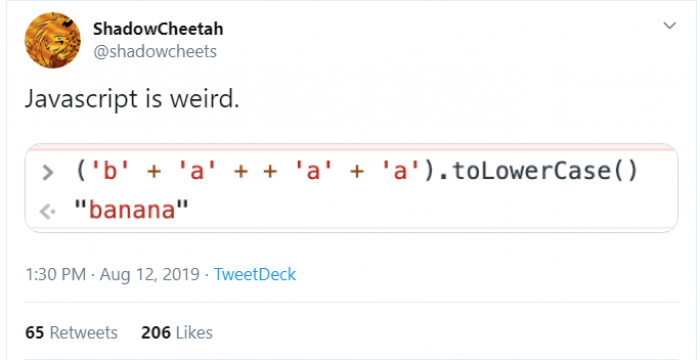
\includegraphics[scale=0.7]{javascript_meme}
\caption{\footnotesize{Internet "meme" about the JavaScript language.}}
\captionsetup{aboveskip=0pt,font=it}
\label{fig:javascript_meme}
\end{figure}

\bigskip

\textbf{{\Large Chapter 1.2 Meet WebAssembly}}

\bigskip

After the initial release in 2017, WebAssembly was first adapted by a number of major web browsers [21]. Since then, there has been a growing community built around the technology as more and more projects started using WebAssembly. As mentioned above, JavaScript have been the de facto language for web browsers since the beginning of the web. However, this was never the original intention during the development of JavaScript.

WebAssembly is the first widely adopted language that was built entire from the ground up with a formal semantics, and it was designed to work in areas it originally intended, which is large, complex apps running on modern web browsers. WebAssembly have an incredibly clean, simple yet powerful design such as memory allocation and garbage collection [21]. However, WebAssembly is actually a form of binary code. Developers and engineers don't usually write WASM code directly, instead they write programs with other low-level languages such as c, c++ or rust [29].

One of the biggest advantage for WebAssembly is standardisation. That is, the ability to compile a wide variety of different programming languages down to just one, which can be very useful in a number of different scenarios and is largely missing from today's software development practices. As an example, Java and Python developers cannot work on the same piece of software together as the code compilation method is very different between the two languages. However, when it comes to developing WebAssembly programs, developers from all programming backgrounds now have the ability to work together and contribute to the same piece of software using languages they are comfortable with. A good example 

\bigskip
\bigskip

\textbf{{\Large Chapter 1.3 XXX}}

\bigskip

Test
\chapter{Literature Review} \label{chap:litreview}

The literature review goes in here.


\chapter{Methodology} \label{chap:methodology}

In this section, we will formally introduce our experiment. Including the experiment background, the execution plan, the methods and our approaches, as well as our hypothesis for the experiment. Lastly, the expected outcome.

During our literature review section, we explored and discovered a few recent studies on the performance of WebAssembly. Including the comparison between WebAssembly and JavaScript when running in web browsers and the same comparison on native OS environments. The conclusions from those studies are usually favourable towards Webassembly. In addition, with the real-world use case of integrating WebAssembly into web applications, it is not difficult to conclude that WebAssembly performs better than the current implementation across all use cases. However, in this thesis, we argue that this is not true as there need to be more studies on the performance comparison between WebAssembly and the current implementation running on the server-side. Therefore, we will take on this question and fulfil this gap by conducting our own research and undertaking our own experiment.

\bigskip
\section{Introduction and Background}

From the above chapters, we have introduced the concept of WebAssembly and the runtime environments it is currently able to run on, as well as other related topics. Currently, WebAssembly is a trendy topic within the web development industry, but less so outside of it. Therefore, we can undertake a considerable amount of work and research within this area.

For a very long time, companies and organisations deployed and hosted server-side applications on their own servers. That was until the introduction of \textbf{cloud computing}, also known as \textbf{Platform as a service (PaaS)}. Typical cloud computing service providers include \textbf{Amazon Web Services}, which was released all the way back in \textbf{2006} \cite{eva1}, \textbf{Google Cloud Platform} \cite{eva2}, and \textbf{Microsoft Azure} which was released in \textbf{2008} and \textbf{2010}, respectively \cite{eva3}. Cloud computing eliminated the need for individual companies to run, operate and maintain their own servers. Instead, it provides a solution for companies to publish and deploy their applications off-premise. Therefore, it also eliminates the cost of the initial server construction as well as the maintenance of the server.

However, one major issue of cloud computing is \textbf{security}. Anyone can create an application and use the service from PaaS companies to deploy it to the cloud. Therefore, cloud service providers usually have several security features built into their service. One of the most common security features cloud computing companies adopted is containerising clients' applications to individual containers to prevent the application from interacting with the hosting server's operating system. This is a very effective way to improve security measures. However, our literature review discovered that several researchers suggested running applications in containers/virtual machines resulted in worse app performances.

Despite the shortcomings, the container method is adopted by most cloud services, and it is currently the standard, de facto way of publishing and deploying applications to the cloud.

\bigskip
\section{Motivation}

We focused on edge computing a lot in this thesis. We understand that edge computing is getting more popular every day. According to Google searches, we are about \textbf{4} times more interested in edge computing than we were just 5 years ago \cite{exp1}. Large information systems and tech companies have also developed their own edge computing frameworks and products, such as \textbf{Google} with Firebase Cloud Functions \cite{exp2}, \textbf{Cloudflare} with Cloudflare workers \cite{exp3} and \textbf{Vercel} - The creator of Next.js \cite{exp4}, one of the most popular web frameworks, recently entered the edge computing market by introducing edge function for the framework \cite{exp5}.

\newpage
\bigskip
\begin{figure}[hp]
\centering
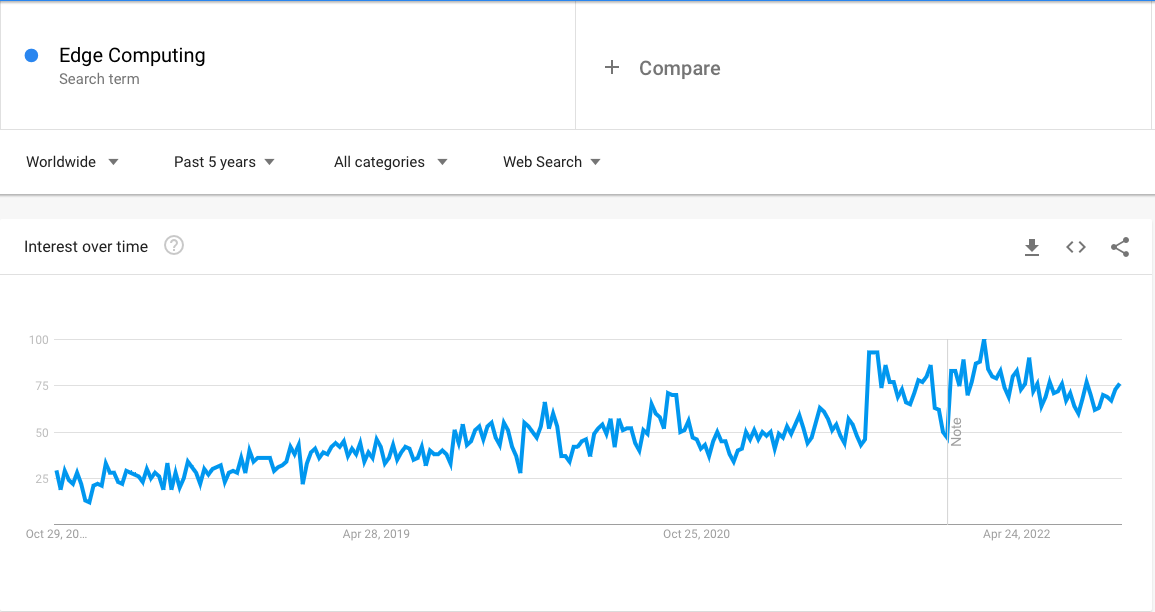
\includegraphics[scale=0.35]{edge-computing-trends}
\caption{\footnotesize{Google trends for edge computing \cite{exp1}}}
\captionsetup{aboveskip=0pt,font=it}
\end{figure}
\bigskip

However, with the current implementation, hosting server-side applications on edge is very inefficient. For example, according to Gadepalli et al. \cite{exp6}, the majority of the current implementation approach is either \textbf{VM-Based (Virtual Machine)} or \textbf{Container-Based}.

For the VM-Based approach, each application is hosted in separate virtual machines within physical hardware. Each virtual machine consists of its own operating system, kernel resource management, library dependencies and language runtimes. These resources will then be utilised to run the application deployed from the client. On the top level, the physical hardware, usually known as a VM manager, manages each of these virtual machines by distributing memory and CPU resources as well as watching the processing thread. This approach is used by a number of well-known cloud service providers. For example, AWS Lambda and Azure Functions \cite{exp7} \cite{exp8}.

The Container-Based implementation uses a more straightforward structure than the VM-Based implementation. With a Container-Based solution, each application will be hosted in containers as per the name suggested. Each container also contains its own library dependencies as well as language runtimes. However, unlike the virtual machine approach, containers have direct access to the hardware's memory and CPU, as well as limited access to specific system APIs. With this method, applications are no longer hosted in virtual machines. Therefore it usually has a faster cold start latency than the VM-Based approach. Popular services such as \textbf{Google Cloud Function} and \textbf{Apache OpenWhisk} use this approach \cite{exp9} \cite{exp10}.

After getting familiarised with the current technology, my natural research instinct kicked in. I kept asking myself if this could be looked into and perhaps researched and experimented with. From all the readings and literature reviews, it is easy to assume that WebAssembly simply has a better performance than the current technology, including when running on the edge. However, we have yet to find the answer, as this is only an assumption. Therefore, we are interested in comparing the two's performances, and we would like to conduct experiments in the environments and scenarios described above.

\begin{figure}[hp]
\centering
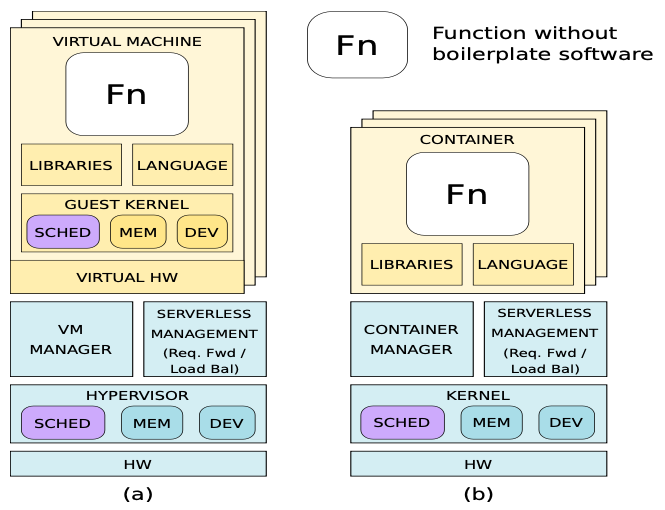
\includegraphics[scale=0.5]{sledge-design-a-b}
\caption{\footnotesize{Visualisation of the current edge computing system design layout, \textbf{a}: VM-Based implementation, \textbf{b}: Container-Based implementation \cite{exp6}}}
\captionsetup{aboveskip=0pt,font=it}
\end{figure}
\bigskip

\bigskip
\section{Our Experiment Goals}

Our experiment involves \textbf{comparing}, \textbf{benchmarking}, and \textbf{analysing} the difference in performance on several aspects between the current way of implementing server-side applications on the cloud, with the newly proposed method of running them with the help of WebAssembly on edge. At the end, we will provide a set of benchmarks that includes the analysed data of the experiment we conducted to contribute to the design and implementation of future commercial WebAssembly frameworks.

Furthermore, we will be listing out and discussing the issues we encountered during our experiment and providing solutions to them to help further research avoid them and improve their research productivity and output.

\bigskip
\section{Improvements and Contribution}

As mentioned above, the current way of developing and deploying server-side applications is neither the most efficient nor cheapest. Applications wrapped in containers while being deployed to a remote server, sometimes on the opposite side of the world, add a considerable amount of \textbf{Round-trip time (RTT)} delay as well as computing overhead. In contrast, the new way of implementation has shown its potential to increase performance by having less overhead and decreasing RTT delay by being distributed on the edge network to be closer to users' physical locations.

We have seen studies showing that when running inside web browsers, WebAssembly outperforms JavaScript on a number of operations and scenarios. This is also reflected by the increasing industry adoption of the technology, with big-name companies such as \textbf{Google} and \textbf{Adobe} migrating major projects from JavaScript to WebAssembly. But, there are very few examples for WebAssembly frameworks being considered and used outside of web browsers, and they have yet to gain too much attention within the industry.

However, this has been changing recently. Multiple studies from the last two years have proposed the idea of running WebAssembly microservices on the server-side and the benefit of doing so. They also developed their own WebAssembly microservice frameworks. In our experiment, we will pick a WebAssembly framework from those implementations and compare that with one of the most popular server-side web frameworks - Python Flask \cite{eva4}.

\newpage
\bigskip
\begin{figure}[hp]
\centering
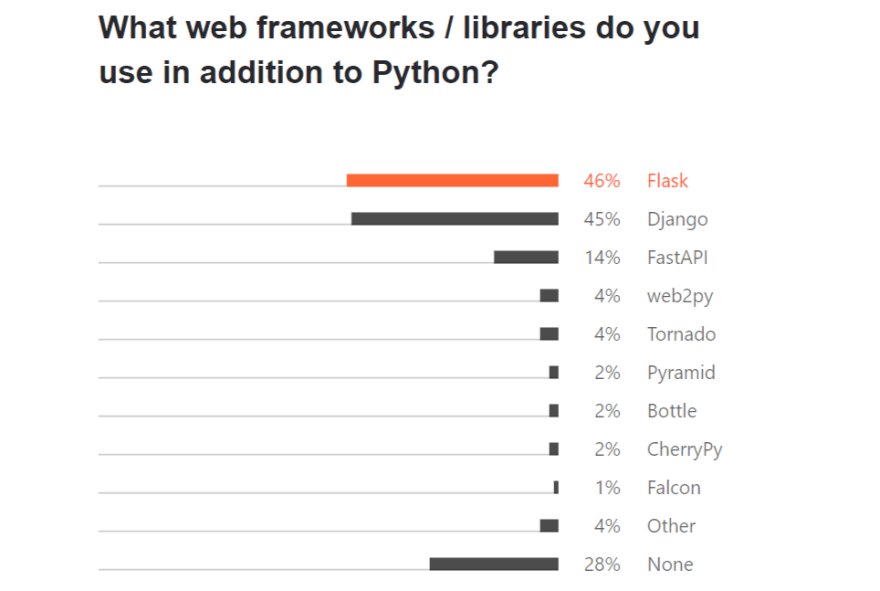
\includegraphics[scale=0.4]{hg2dcbj3lvu2jbjjtdd4}
\caption{\footnotesize{Popularity of major Python web frameworks \cite{eva4}}}
\captionsetup{aboveskip=0pt,font=it}
\end{figure}
\bigskip

\bigskip
\begin{figure}[hp]
\centering
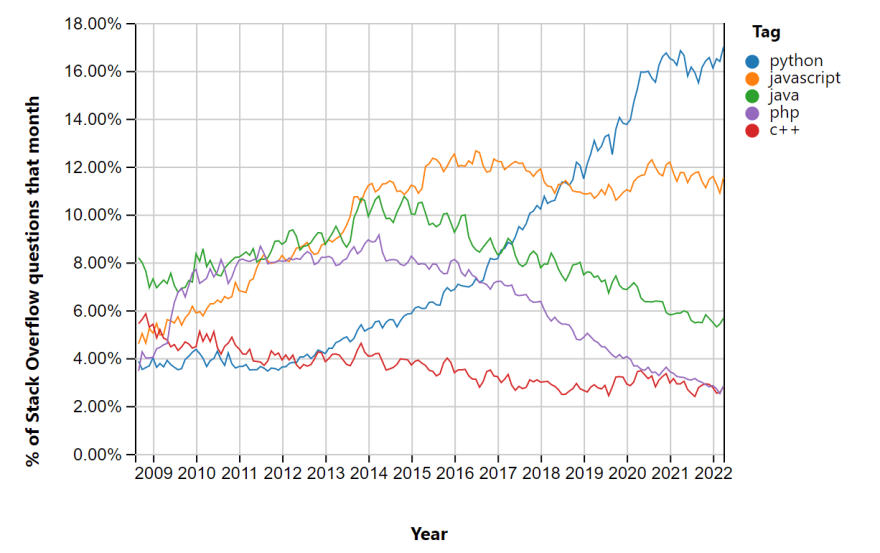
\includegraphics[scale=0.4]{s4fwpypy7bkvtt9kcgr1}
\caption{\footnotesize{Popularity of major programming languages \cite{eva4}}}
\captionsetup{aboveskip=0pt,font=it}
\end{figure}
\bigskip

\bigskip
\section{Hypothesis and Excepted Results}

Since we are undertaking the experiment to either solidify or disprove our expected outcome, we have come up with our own hypothesis for the investigation. From the research and literature review we have undertaken, we understand that WebAssembly has a better performance than JavaScript in web browsers, as well as a faster "code-start" time and lower overhead when running on the server-side. Furthermore, it has a solid technical community to issue updates and patches regularly, as well as work on runtime efficiency and overhead reduction. This resulted in the technology getting more widely adopted as time moved on. Therefore, we consider WebAssembly to be a serious contender in the future of commercial server-side development. And we expect to see a better performance towards the WebAssembly framework in our experiment. We will present our hypothesis in greater detail in the upcoming experiments section.
\chapter{Background} \label{chap:background}

In this section, we will introduce the background leading to the experiment. For example, the different kinds and types of web frameworks. We will also introduce the environment leading to the experiment.

\section{Expanding on the Experiment Background}

From the above section, we stated that during the framework benchmarking experiment, we expect the WebAssembly framework to come out on top from various benefits it provides, such as a lower computation overhead and better RTT delays.

Our experiment will first be conducted in a controlled environment. Depending on the result we receive from this investigation stage, we then decide what the next phase of our experiment will be. This can either be designing, implementing and carrying out a "real-life" scenario experiment with both frameworks. Or to expand, understand and conduct further research into the potential irregularities observed within the collected data from the first stage of the investigation.

This way, we will be extra confident with the data we collected from the experiment. Therefore, we shall have a stronger argument when communicating our results and findings to other researchers and engineers, as well as ensuring that the results we get are as accurate as possible.

\section{Further Understanding of client-side application and server-side application}

A web framework, sometimes also referred to as a web application framework, is a collection of functionalities and libraries engineered and designed to lay the groundwork and provide basic infrastructures and logic for applications to be built on top of. This way, developers and engineers working on the project do not have to implement such functionalities themselves. It simplifies the development process, reduces development time and increases development productivity output \cite{exp11}.

There are usually two web framework categories: \textbf{client-side} and \textbf{server-side}. The former is generally used in order to construct dynamic web applications \cite{exp12}, while the latter is usually used to develop backend API services. According to the \textbf{2022 annual developer survey from stack overflow} \cite{exp20}, some of the most popular client-side frameworks including \textbf{React.js} \cite{exp13}, \textbf{Angular} \cite{exp14} and \textbf{Vue.js} \cite{exp15}, while some of the most popular server-side frameworks including \textbf{Node.js} \cite{exp16}, \textbf{ASP.NET} \cite{exp17} and \textbf{Django} \cite{exp18} (server-side Django REST framework) \cite{exp19}.

It has been mentioned in multiple research articles that running complete web applications using the current cloud solution may produce too much overhead, thus leading to inefficiency. For example, Gackstatter \cite{exp21} recognises the limitation of today's "cloud-centric model" when it comes to deploying web applications at the edge. Specifically, the author stated that applying the current solution, such as virtual machines and containers, does not promise an effective solution due to the limited resources available. Additionally, Gadepalli et al. not only pointed out the wide adoption of the virtual machine/container model, but also stated that server applications built using WASM functions that run naively have the potential to expand the current use case of comprehensive applications running from the edge due to the reduction of the overhead which reduces the response time down to within \textbf{10} milliseconds \cite{exp6}.

With the current model of implementation, \textbf{Docker} \cite{exp22} and \textbf{Kubernetes} \cite{exp23} are usually used in the publishing process to prepare an application for edge deployment. In this case, it would "wrap" the application into containers which will be further deployed onto self-managed serverless infrastructures or cloud computing service providers that provide edge services such as \textbf{Amazon Web Service} or \textbf{Microsoft Azure}. Those services will then distribute the application to edge devices across data centres worldwide.

My research aims to study and uncover the current state of WebAssembly frameworks running on the edge, which is to run functions as microservices directly from the native operating system using WebAssembly through a WASM runtime, and its performance gap and inconsistency with traditional VM-based implementations. This includes applications developed and deployed with virtual machines, containers and conventional language runtimes.

Currently, at this stage, the true performance capability of WebAssembly has yet to be fully realised due to the relatively short time it has been around compared to JavaScript - which has almost \textbf{30} years of development ahead of it. However, it is apparent to us that WebAssembly has a huge potential in terms of its performance both when running in web browsers as well as running on operating systems naively through a runtime. We can back this up with the performance data of JavaScript over the years. In a presentation, Verschore presented a figure which stated that between 2001 and 2009, there was a \textbf{100} times improvement in JavaScript's performance as well as considerable increases in the browser Octane score (web page loading speed) \cite{exp24}.

\bigskip
\begin{figure}[!ht]
\centering
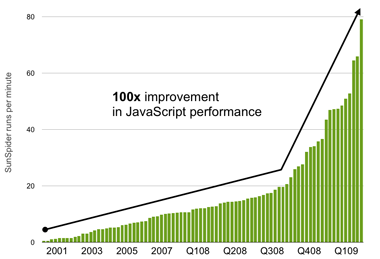
\includegraphics[scale=0.7]{js-perf}
\caption{\footnotesize{SunSpider benchmark score for the SpiderMonkey engine, which is used in Firefox \cite{exp24}}}
\captionsetup{aboveskip=0pt,font=it}
\end{figure}
\bigskip

On top of that, the V8 JavaScript engine \cite{int31} behind popular browsers such as Google Chrome \cite{exp25} and Brave \cite{exp26} also had an incredible journey from when it was first released to the public back in 2008. The V8 development team undertook and released a set of benchmark scores comparing the performance of the Chrome browser from its original beta to the versions in 2018. The results showed that in just 10 years, both its V8 Bench score \cite{exp27} and Speedometer score \cite{exp28} increased by \textbf{4} times, and the engine had also became a lot more stable as well as added support for a lot more chip architectures such as \textbf{ARM} and \textbf{ARM 64} \cite{exp29} \cite{exp30}.

\newpage
\bigskip
\begin{figure}[hp]
\centering
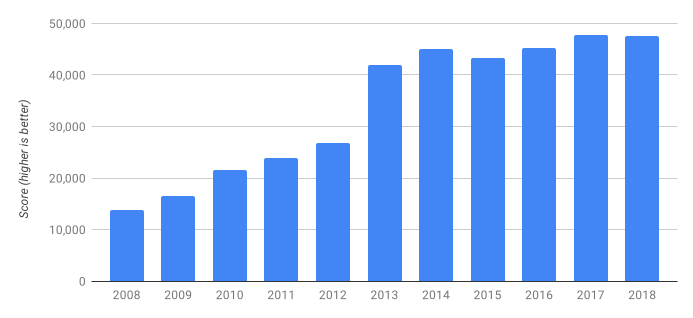
\includegraphics[scale=0.5]{chrome-v8-bench}
\caption{\footnotesize{Google Chrome's V8 Bench score between its original beta and the version in 2018 \cite{exp29}}}
\captionsetup{aboveskip=0pt,font=it}
\end{figure}
\bigskip

\bigskip
\begin{figure}[hp]
\centering
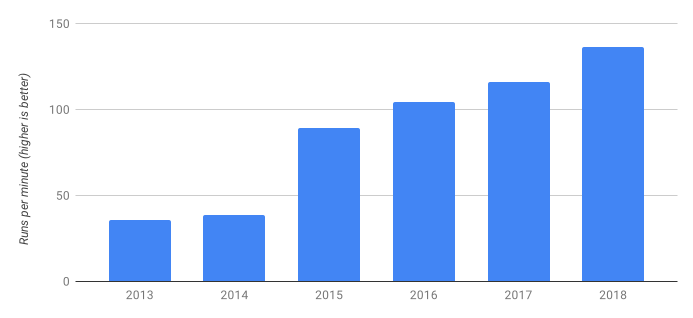
\includegraphics[scale=0.5]{chrome-speedometer-1}
\caption{\footnotesize{Google Chrome's Speedometer 1 score between its original beta and the version in 2018 \cite{exp29}}}
\captionsetup{aboveskip=0pt,font=it}
\end{figure}
\bigskip

One recent example is the new \textbf{Bun.js} JavaScript runtime \cite{exp31}. It is a newly released JS runtime at the time of writing. It was built with prior experience with Node.JS and made several visible improvements on top of that. Namely adding the support for edge computing.

\bigskip
\begin{figure}[hp]
\centering
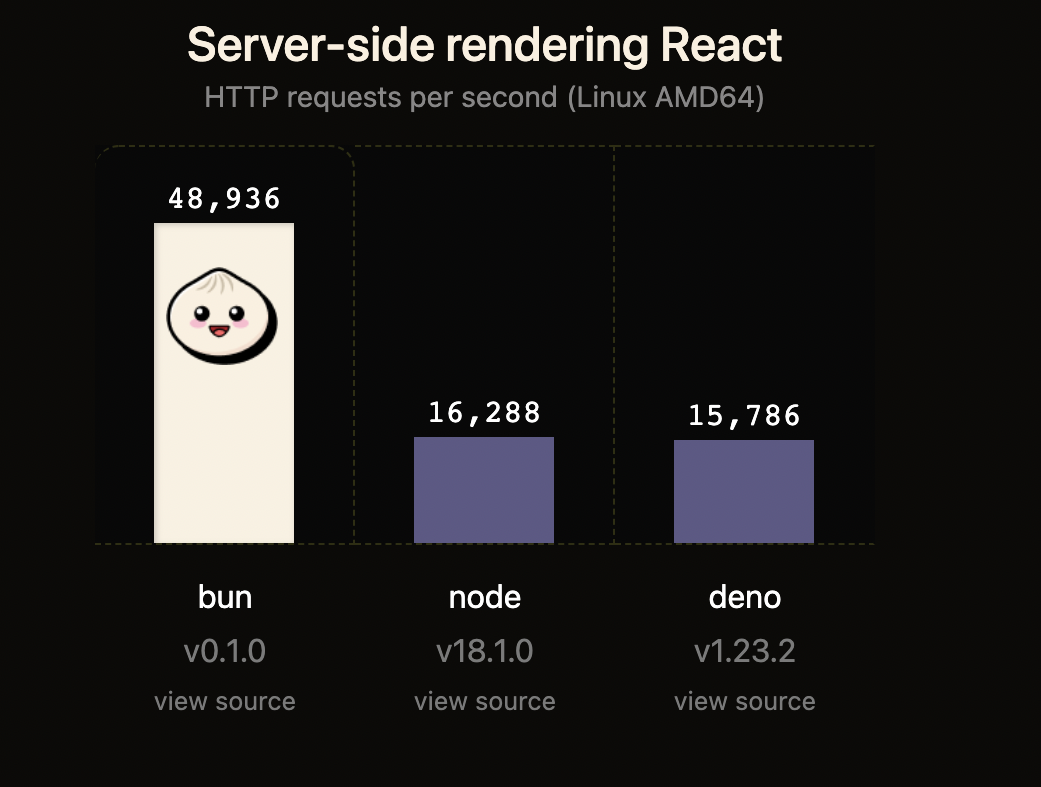
\includegraphics[scale=0.35]{bun-comparison}
\caption{\footnotesize{Performance comparison on HTTP requests between Bun and Node.JS \cite{exp31}}}
\captionsetup{aboveskip=0pt,font=it}
\end{figure}
\bigskip
\chapter{Experiments} \label{chap:experiments}

In this section, we will be introducing the experiment we are conducting as well as showcasing different steps we are undertaking in order to conduct our experiment among a few other things. For example, the background and summary for different kinds and types of web frameworks. Firstly, we will introduce the background leading to the experiment and the motivation behind the experiment. After that, we will list out our detailed goals, hypothesis and expectations from the experiment as well as our hardware and software environment configuration. Then, we will setup and start conducting the experiment while simultaneously explaining and justifying each of the steps during the process.

After the experiment, we will first collect all the data that was produced from the experiment. We will than start analysing and categorising the collected data, process them and present them in the "Result" section. Furthermore, we will provide our verdict of the experiment by delivering discussions on the experiment itself such as whether the result was largely within our expectation or perhaps the results differs from our initial assumption and prediction by a considerable margin.

Finally, we will list the challenges we faced and the irregularities we found during our experiment, as well as possible future work that might be worth undertaking in the "Discussion" section.

\bigskip
\section{Expending on the Experiment Background}

From the evaluation section above, we stated that during the framework benchmarking experiment, we expect the WebAssembly framework to come out on top from a variety of benefits it provides. Such as a lower computation overhead and better RTT delays.

Our experiment will first be conducted in a controlled environment. Depends on the result we receive from this stage of the experiment, we then decide what the next stage of our experiment will be. This can either be designing, implementing and to carry out a "real-life" scenario experiment with both frameworks, or to expend, understand and conduct further research into the potential irregularities observed within the collected data from the first stage of the experiment.

This way, we will be extra confident with the data we collected from the experiment. Therefore, we shall have a stronger argument when communicating our results and our findings to other researchers and engineers, as well as making sure that the results we get are as accurate as possible.

\bigskip
\textbf{{\Large Chapter 4.2 Motivation}}

We focused on edge computing a lot in this thesis, we understand that edge computing is getting more popular everyday. According to Google searches, we are about 4 times more interested in edge computing than we were just 5 years ago [34]. Large information systems and tech companies have also developed their own edge computing frameworks and products, such as Google with Firebase Cloud Functions [35], Cloudflare with Cloudflare workers [36] and Vercel - The creator for Next.js [37], one of the most popular web frameworks, recently entered the edge computing market by introducing edge function for the framework [39].

\bigskip
\begin{figure}[hp]
\centering
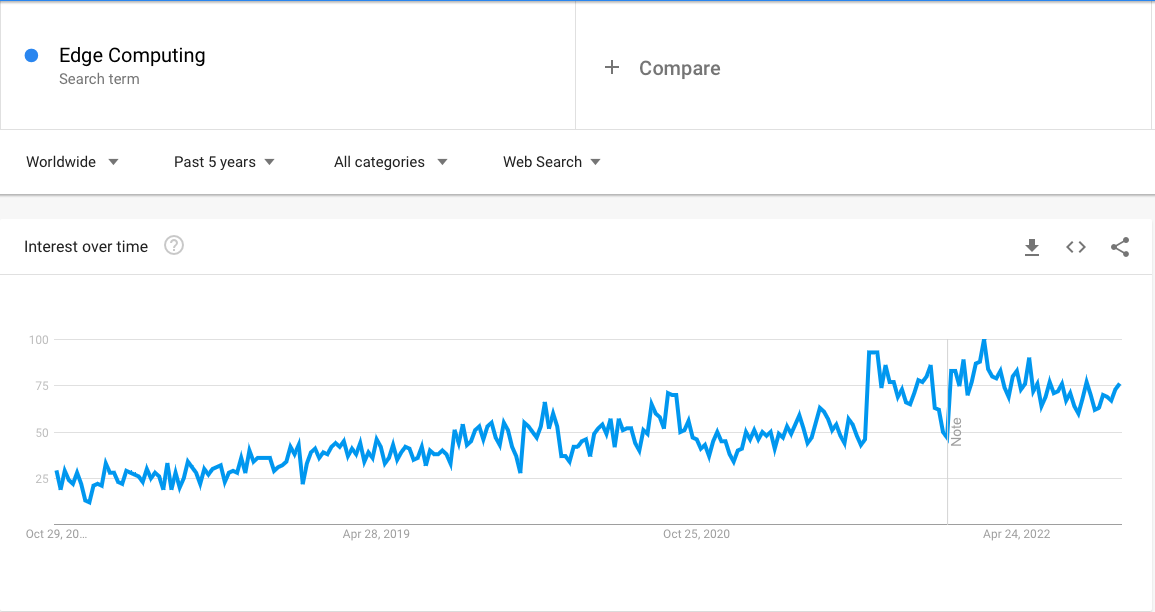
\includegraphics[scale=0.35]{edge-computing-trends}
\caption{\footnotesize{Google trends for edge computing}}
\captionsetup{aboveskip=0pt,font=it}
\end{figure}
\bigskip

However, with the current implementation, hosting server-side applications on the edge is just very inefficient. For example, according to Gadepalli et al. [39], the majority of the current implementation approach is either VM-Based (Virtual Machine) or Container-Based.

For VM-Based approach, each application are hosted in separate virtual machines within a physical hardware. Each virtual machine consists of its own operating system, kernel resource management, library dependencies and language runtimes. All of these resources will than be utilised to run the application deployed from the client. On the top level, the physical hardware usually known as a VM manager manages each of these virtual machines by distributing memory and CPU resources and over watching the processing thread. This approach is used by a number of well-known cloud service providers. For example, AWS Lambda and Azure Functions [40] [41].

Container-Based implementation uses a more straight forward structure than VM-Based implementation. With Container-Based implementation, each applications will be hosted in containers as per name suggested. Each containers also contains its own library dependencies as well as language runtimes. However, unlike the virtual machine approach, containers have direct access to the hardware's memory and CPU as well as limited access to certain system APIs. With this method, applications are no longer hosted in virtual machines, therefore it usually have a faster cold start latency than VM-Based approach. Popular services such as Google Cloud Function and Apache OpenWhisk uses this approach [42] [43].

After getting familiarised with the current technology, my natural research instinct kicked in, I kept asking myself if this is something that can be looked into and perhaps to be researched and experimented. From all the readings and literature reviews, it is easy to assume that WebAssembly simply has a better performance than the current technology including when running on the edge. However, we don't know the answer yet as this is only an assumption. Therefore, we are interested in comparing the performance between the two and we would like to conduct experiments in environments and scenarios described above.

\newpage
\begin{figure}[hp]
\centering
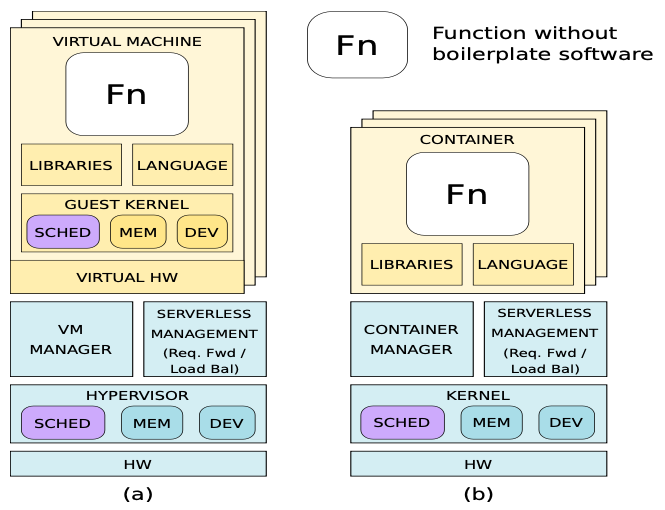
\includegraphics[scale=0.5]{sledge-design-a-b}
\caption{\footnotesize{Visualisation of the current edge computing system design layout, \textbf{a}: VM-Based implementation, \textbf{b}: Container-Based implementation}}
\captionsetup{aboveskip=0pt,font=it}
\end{figure}
\bigskip

\textbf{{\Large Chapter 4.3 Further Understanding on client-side application and server-side application}}

A web framework, sometimes also referred as a web application framework, is a collection of functionalities and libraries that is engineered and designed with the intention of laying the groundwork and providing basic infrastructures and logic for applications to be built on top of. This is so that developers and engineers working on the project do not have to implement such functionalities themselves. it simplifies the development process, reduces development time and increases development productivity output [44].

There are usually two categories of web frameworks: client-side framework and server-side framework. The former is usually used in order to construct dynamic web applications [45] while the latter is usually used to develop back-end API services. According to the 2022 annual developer survey from stack overflow [53], some of the most popular client-side frameworks including React.js [46], Angular [47] and Vue.js [48] while some of the most popular server-side frameworks including Node.js [49], ASP.NET [50] and Django [51] (server-side Django REST framework) [52].

It has been mentioned in multiple research articles that running full web applications using the current cloud solution may produce too much overhead, thus leads to inefficiency. For example, Gackstatter [54] recognise the limitation of today's "cloud-centric model" when it comes to deploying web applications at the edge. Specifically, the author stated that applying the current solution such as virtual machines and containers does not promise to be an effective solution due to limited resources available. Additionally, Gadepalli et al. not only pointed out the widely adoption of the virtual machine/container model, but also stated that server applications built using WASM functions that runs naively have the potential to expand the current use case of comprehensive applications running from the edge due to the reduction of the overhead which reduce the respond time down to within 10 milliseconds [39].

With the current model of implementation, Docker [77] and Kubernetes [78] are usually used in the publishing process in order to prepare an application for edge deployment. This would "wrap" the application into containers which will be further deployed onto self-managed serverless infrastructures or cloud computing service providers that provide edge services such as Amazon Web Service or Microsoft Azure. Those services will then distribute the application to edge devices across data centres around the world.

The topic and question of my research is to discover the performance gap and inconsistency between the current implementation of edge applications which includes application development and deployment with virtual machines, containers and traditional language runtimes, with the proposed WebAssembly solution which is to run functions as microservices directly from the native operating system using WebAssembly through a WASM runtime.

Currently at this stage, the true performance capability of WebAssembly has not yet been fully realised due to the relatively short time it has been around in comparison to JavaScript - which has almost 30 years of development. However, it is apparent to us that WebAssembly have a huge potential in terms of it's performance both when running in web browsers as well as running on operating systems naively through a runtime. We are able to back this up with the performance data of JavaScript over the years. In a presentation, Verschore presented a figure which stated that between 2001 and 2009, there was an 100-times improvement in JavaScript's performance as well as huge increases in the browser Octane score (web page loading speed) [55].

\newpage
\begin{figure}[!ht]
\centering
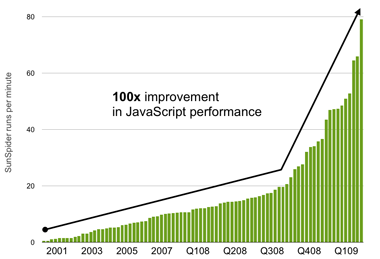
\includegraphics[scale=0.7]{js-perf}
\caption{\footnotesize{SunSpider benchmark score for the SpiderMonkey engine which is used in Firefox}}
\captionsetup{aboveskip=0pt,font=it}
\end{figure}

On top of that, the V8 JavaScript engine [58] behind popular browsers such as Google Chrome [56] and Brave [57], also had an incredible journey from when it was first released to the public back in 2008. The V8 development team undertook and released a set of benchmark scores comparing the performance of the Chrome browser from it's original beta to the versions in 2018. The results showed that in just 10 years, both its V8 Bench score [59] and Speedometer score [60] increased by 4 times, and the engine had also became a lot more stable as well as added support for a lot more chip architectures such as ARM and ARM 64 [61] [62].

\bigskip
\begin{figure}[hp]
\centering
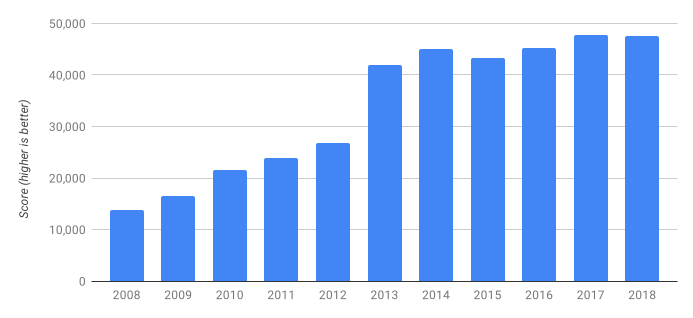
\includegraphics[scale=0.5]{chrome-v8-bench}
\caption{\footnotesize{Google Chrome's V8 Bench score between its original beta and the version in 2018}}
\captionsetup{aboveskip=0pt,font=it}
\end{figure}

\newpage
\begin{figure}[hp]
\centering
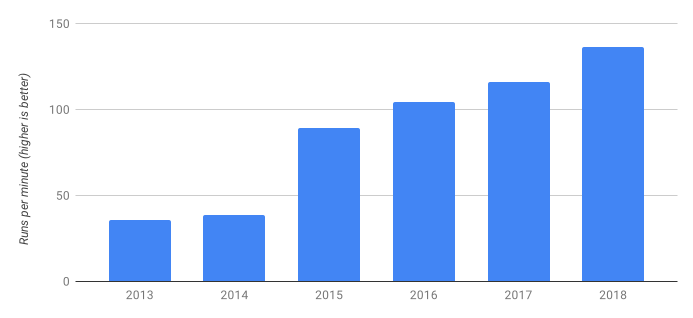
\includegraphics[scale=0.5]{chrome-speedometer-1}
\caption{\footnotesize{Google Chrome's Speedometer 1 score between its original beta and the version in 2018}}
\captionsetup{aboveskip=0pt,font=it}
\end{figure}
\bigskip

One of the recent example is the new Bun.js JavaScript runtime [79]. It is a newly released run time at the time of writing. It was build with the prior experience of Node.JS and made several visible improvements on top of that. Namely adding the support for edge computing.

\bigskip
\begin{figure}[hp]
\centering
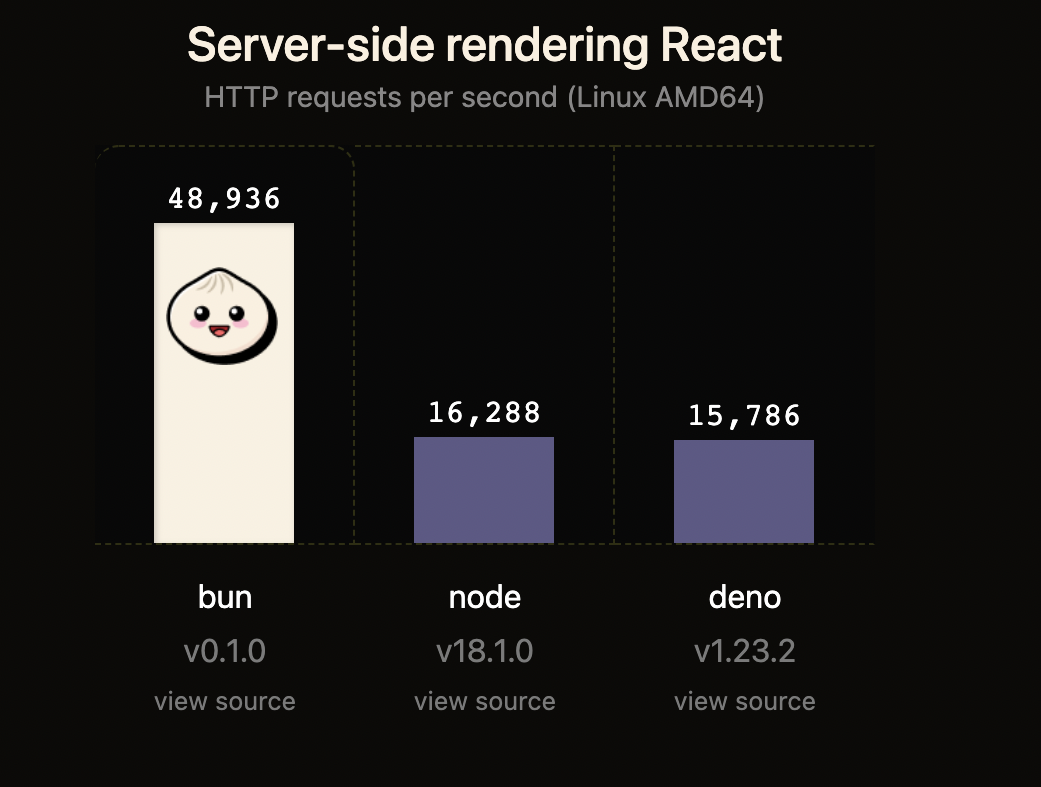
\includegraphics[scale=0.35]{bun-comparison}
\caption{\footnotesize{Performance comparison on HTTP requests between Bun and Node.JS}}
\captionsetup{aboveskip=0pt,font=it}
\end{figure}
\bigskip

\bigskip
\textbf{{\Large Chapter 4.4 WebAssembly framework options}}

Our experiment will focus on the two categories of microservice frameworks: VM/Container based frameworks and WebAssembly based frameworks. In addition, with each experiment scenarios, we will run it in our local environment as well as on the cloud computing server.

Here are some of the WebAssembly frameworks we are interested in. In this section, we will compare and analyse and in addition, to identify the strengths, weaknesses as well as characteristics for each of the frameworks. At the end, we will choose a framework that aligns with our interests the most.

\bigskip
\begin{table}[h!]
\centering
\begin{tabular}{||c c c||} 
\hline
Name & Developer & Website \\ [1ex] 
\hline\hline
 & & \\
Sledge & George Washington University & github.com/gwsystems/sledge-serverless-framework \\ 
 & & \\
Spin & Fermyon & github.com/fermyon/spin \\
 & & \\
WasmEdge (Runtime) & Linux foundation & wasmedge.org \\
 & & \\
Krustlet (Kubelet) & Deislabs & krustlet.dev \\
 & & \\
WAGI & Deislabs & github.com/deislabs/wagi \\
 & & \\
Wasmcloud & Wasmcloud team & wasmcloud.dev \\ [1ex]
\hline
\end{tabular}
\caption{List of WebAssembly frameworks of interest}
\label{table:webassembly_frameworks}
\end{table}

\bigskip
\textbf{{\normalsize Chapter 4.4.1 Sledge}}

Sledge framework was created and developed by the researchers at George Washington University. It offers a fast yet lightweight user experience and is designed to be run using WebAssembly runtimes natively. On top of that, the researchers have also developed a custom WASM runtime for it, called AWSM [80] (pronounced Awesome) using the Rust language [81]. However, both projects have yet to be production ready and are still in the testing phase. Adding on to that, they have yet to provide an official deployment instruction for the framework.

\bigskip
\textbf{{\normalsize Chapter 4.4.2 Spin}}

The Spin framework by the Fermyon company is one of the most popular server-side WebAssembly frameworks out there at the moment. It is also featured in multiple news articles including Yahoo! Finance [82] and Forbes [83]. Although not fully production ready yet, a considerable amount of testing have been done on the framework and the it has gained a considerable amount of attention within the backend server-side community.

On top of that, Fermyon has implemented and documented a detailed set of deployment instructions for spin. They created their own Platform-as-a-service solution - Fermyon cloud to host and manage Fermyon applications. They also teamed up with Deislabs which is another major company in the WebAssembly server-side market to deploy spin applications to Amazon Web Service through its Hippo bundler.

\bigskip
\textbf{{\normalsize Chapter 4.4.3 WAGI}}

WAGI is a product made by the aforementioned Deislabs. It is a super lightweight WebAssembly HTTP framework in its very early stage of development. WAGI is just like spin in many ways. It is able to compile the code down to WASM32-WASI which is a type of WebAssembly binary code. Therefore, it is able to run with any programming languages that compiles to WASM32-WASI, such as Rust and Go. However, unlike spin, it is only classified as experimental code and Deislabs currently does not have the plan to further develop WAGI into a production ready product. It also does not have an official deployment method.

\bigskip
\textbf{{\normalsize Chapter 4.4.4 Wasmcloud}}

Wasmcloud is a server-side backend framework and runtime that runs on all three major operating systems, Windows, macOS and Linux. On top of that, it is a polyglot platform which allows the same application being developed using multiple programming languages. In this case, AssemblyScript, Go or Rust. It was designed with security and scalability in mind. It also functions as an ecosystem where each functions are called "actors", Wasmcloud provides it's own Paas cloud computing service to deploy server-side applications, IoT applications as well as client-side applications running in web browsers. Furthermore, it has built-in edge support and has a detailed set of instruction and documentation on the deployment procedure.

\bigskip
\textbf{{\Large Chapter 4.5 Decision on Frameworks and Environment }}

We start by choosing a WebAssembly framework. We looked at the properties of the WebAssembly frameworks above and we decided to go with Spin by Fermyon. There are a few reasons contributing to this decision. Spin has a very detailed set of documentation as well as example projects. More crucially, there exists a research gap here as there hasn't been any tests performed on spin running on the edge.

On the other hand, the other non-WebAssembly traditional framework we will be utilising into our experiment is Flask [52]. As stated above, Flask is a Python HTTP microservice framework. It is currently one of the most popular traditional non-Webassembly frameworks and Python is also one of the most popular programming language.

The local environment for conducting our experiments will be on a 2017 MacBook Pro running with the Intel Core I5-7267U CPU (2 cores, 3.1 GHz), it has an 8GB memory with 512GB internal SSD storage. For the production environment, we will be using Amazon Web Service for our cloud and edge deployment. Specifically, we will be utilising the Amazon EC2 service to host our applications [87]. Amazon EC2 offers a wide range of instances (server computers) that suits the need for most businesses ranging from small IoT controller computers to large industrial servers for server farms [88]. In our case, both of our frameworks will be deployed and run on an AWS t3 micro instance. The t3 micro instance is a medium rage server. It has 2 vCPUs (Intel Xeon or AMD EPYC, both running up to 3.1 GHz) with 1GB memory and on-demand elastic storage (it charge its customers based on the amount of storage it holds). It is designed to run applications such as microservices, small to medium databases, business critical applications and so on [89]. It is small yet agile enough to be used as an edge server for our spin application, but also powerful enough to host our flask application for it to run in a traditional cloud environment.

\bigskip
\textbf{{\Large Chapter 4.6 Roadblocks in Early Stage of Experiment}}

The initial experiment plan is very distinct from the plan described in this section. In the early stage of carrying out the experiment, we planned to integrated PolyBench/C into our benchmarking experiment [93]. PolyBench is one of the best system benchmarking frameworks at the moment and it is originally written in C and the Fortran language by Louis-Noel Pouchet at The Ohio State University [94]. At first, we looked into benchmarking both of our frameworks with PolyBench/Python [95]. Which is a re-implementation of the original PolyBench/C developed by Abella-Gonzalez et al. at the University of A Coruna in Spain alongside with Louis-Noel Pouchet himself. However, when browsing through the project code, we discovered that PolyBench/Python is only available for x86 architecture machines running with Linux due to a number of runtime dependencies only available on the Linux operating system. We initially do not have access to such machines but we later installed a copy of Ubuntu Linux operating system as a virtual machine through Oracle VM VirtualBox [96] [97]. However, at the end, we decided that we won't go ahead with PolyBench/Python due to the potential system compatibility issues we might have on deployment. Therefore, we continued our experiment with the original PolyBench/C framework.

\bigskip
\begin{figure}[hp]
\centering
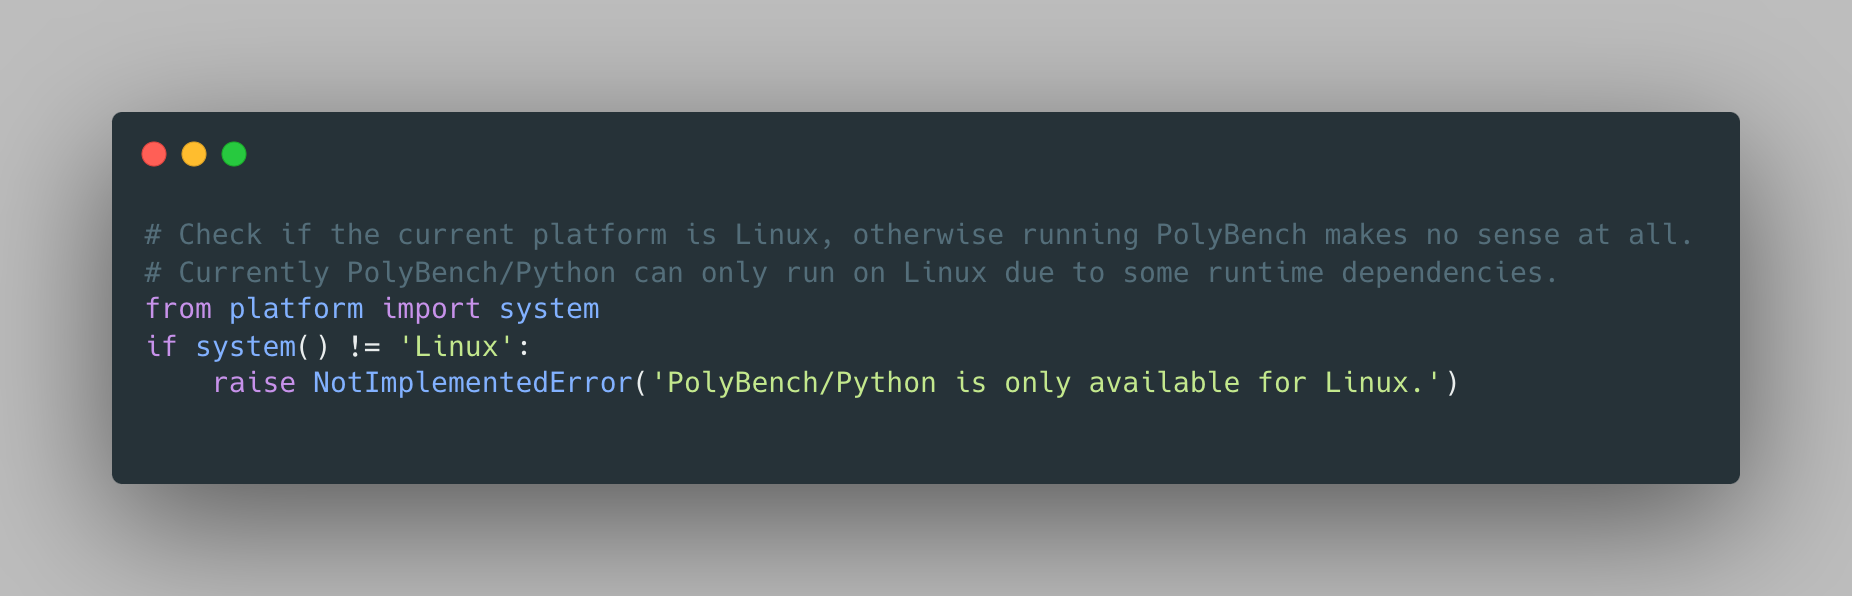
\includegraphics[scale=0.24]{polybench-python}
\caption{\footnotesize{Code snippet on PolyBench/Python compatibility}}
\captionsetup{aboveskip=0pt,font=it}
\end{figure}
\bigskip

There are 30 benchmarking tests in PolyBench/C, its operation covers the majority of everyday computing tasks. PolyBench/C includes numerical computations extracted from various applications. This includes: linear algebra, image processing, physics simulation, dynamic programming, statistics and so on. Each benchmark tests includes a single C program file along with its header H file. User runs the benchmark file by first compiling it to a UNIX executable file with a C compiler such as gcc or clang [98] [99]. After that, they can then generate the output of the program by running it in a terminal application as well as passing in the desired name of the output file. Users can also pass in extra configuration options to alter the compilation process as well as the desired output. For example, to display the program execution time or to change the input dataset size.

The source code of the project can be found here: \href{https://web.cse.ohio-state.edu/~pouchet.2/software/polybench/}{\color{blue}{The Polyhedral Benchmark Suite}}. Here is a list of all benchmark tests (Version 4.2.1) and their descriptions:

\bigskip
\begin{table}[h!]
\centering
\begin{tabular}{||c c||} 
\hline
Name & Description \\ [1ex] 
\hline\hline
 & \\
2mm & 2 Matrix Multiplications (alpha * A * B * C + beta * D) \\ 
 & \\
3mm & 3 Matrix Multiplications ((A*B)*(C*D)) \\ 
 & \\
adi & Alternating Direction Implicit solver \\ 
 & \\
atax & Matrix Transpose and Vector Multiplication \\ 
 & \\
bicg & BiCG Sub Kernel of BiCGStab Linear Solver \\ 
 & \\
cholesky & Cholesky Decomposition \\ 
 & \\
correlation & Correlation Computation \\ 
 & \\
covariance & Covariance Computation \\ 
 & \\
deriche & Edge detection filter \\ 
 & \\
doitgen & Multi-resolution analysis kernel (MADNESS) \\ 
 & \\
durbin & Dynamic programming (2D) \\ 
 & \\
dynprog & Toeplitz system solver \\ 
 & \\
fdtd-2d & 2-D Finite Different Time Domain Kernel \\ 
 & \\
gemm & Matrix-multiply C=alpha.A.B+beta.C \\ 
 & \\
gemver & Vector Multiplication and Matrix Addition \\ 
 & \\
gesummv & Scalar, Vector and Matrix Multiplication \\ [1ex]
\hline
\end{tabular}
\caption{PolyBench/C Benchmarks}
\label{table:time_complexity_2}
\end{table}

\begin{table}[h!]
\centering
\begin{tabular}{||c c||} 
\hline
Name & Description \\ [1ex] 
\hline\hline
 & \\
gramschmidt & Gram-Schmidt decomposition \\ 
 & \\
head-3d & Heat equation over 3D data domain \\ 
 & \\
jacobi-1D & 1-D Jacobi stencil computation \\ 
 & \\
jacobi-2D & 2-D Jacobi stencil computation \\ 
 & \\
lu & LU decomposition \\ 
 & \\
ludcmp & LU decomposition followed by Forward Substitution \\ 
 & \\
mvt & Matrix Vector Product and Transpose \\ 
 & \\
nussinov & Dynamic programming algorithm for sequence alignment \\ 
 & \\
seidel & 2-D Seidel stencil computation \\ 
 & \\
symm & Symmetric matrix-multiply \\ 
 & \\
syr2k & Symmetric rank-2k update \\ 
 & \\
syrk & Symmetric rank-k update \\ 
 & \\
trisolv & Triangular solver \\ 
 & \\
trmm & Triangular matrix-multiply \\ [1ex]
\hline
\end{tabular}
\caption{PolyBench/C Benchmarks (continued 1)}
\label{table:time_complexity_2}
\end{table}

We continue our experiment by start utilising the PolyBench/C code. We designed a program that compiles and execute all 30 algorithms with 5 difference set of data sizes: mini, small, medium, large and extra large.

The program will first construct a list of relevant paths of all benchmark files from the pre set dictionary of \mintinline{python}{ALL_FILES}. After that, the program will create an temporary folder in the project root directory called \mintinline{python}{compiled}, it will then compile all benchmarks into compiled UNIX executable binary files using the gcc compiler and store them into the \mintinline{python}{compiled} folder. For each benchmarks, after its compiled, we will run the program with the 5 aforementioned datasets. After running the binary executable files, we can output and log their runtimes. We do this by writing them in a text file with the naming convention (see below) and saving it persistently in a folder named \mintinline{python}{results} also in the project root directory. Finally after all results were collected, we clean up the runtime environment by removing the \mintinline{python}{compiled} folder.

Result file naming convention:
\newline
\mintinline{python}{output-file-<current date and time (Day-Month-Year-Hour-Minute-Second)>.txt}

The program source code is available publicly on GitHub.
\newline
The link can be found \href{https://github.com/richard875/Honours-PolyBench}{\color{blue}{here (GitHub: richard875/Honours-PolyBench)}}

After developing the PolyBench testing project, we are ready to integrate it with our testing frameworks. The PolyBench testing project was designed to be used as a "module". We achieve this by implementing and exposing a \mintinline{python}{main} function that can be called externally and returns the runtime benchmark data.

We first integrate it with the flask framework, we develop and configure the project so that it calls the \mintinline{python}{main} function on receiving a connection on a particular route, in this case the index \mintinline{python}{/} route, then return and display the timing data on render.

We then integrate it with the spin WebAssembly framework. We did largely the same with the flask framework. We also point the index route to execute the \mintinline{python}{main} function. However, this time the program failed to execute and the benchmarks did not compile.

After conducting further research, we found that it is an expected behaviour for WebAssembly frameworks. As stated in the literature review section, one of the main benefits of WebAssembly is its security. WebAssembly applications executes in a sandboxed environment that is separated from the host environment and only expose limited APIs that was proven to be safe for developers to use [100]. Therefore, in a WebAssembly environment, code such as \mintinline{python}{os.path.isdir(RUNTIME_OUTPUT_FOLDER)} which checks if a directory exists or \mintinline{python}{shutil.rmtree(RUNTIME_OUTPUT_FOLDER, ignore_errors=True)} which deletes a directory folder along with all its contents will not work.

Therefore, we had to stop pursuing this experiment path and change our experiment direction.

\bigskip
\textbf{{\Large Chapter 4.7 Initial Dataset}}

After the previous roadblock, we started to look for other benchmarking solutions. After further researches, we decided that we will start the experiment with a custom collection of sorting algorithms. Some of the most popular sorting algorithms out there including Bubble sort [84], Insertion sort [85] and Quick sort [86]. Sorting algorithms are an excellent way to benchmark the runtime for individual web frameworks as they don't require any incoming or outgoing connections and thus do not have any external uncontrollable factors. Unlike PolyBench, they do not need to be compiled into as standalone files to be run. Furthermore, sorting algorithms are also available in multiple languages (we will use Python in our case). As such, they can be run in almost any environments.

During our experiment, we found that it is very difficult to come up with a set of "one-fits-all" number list input. For instance, some sorting algorithms in our collection take massively longer to complete than others.

We define our list input size (number of elements in the input list) as \(N\). We than set \(N = 1000\) and run the algorithm in local environment. Faster sorting algorithms such as Quick sort and Merge sort took 0.002s and 0.004s to run respectively, while slower sorting algorithms such as Gnome sort and Brick sort took 0.123s and 11.171s respectively (tested under local environment).

Here is a list of 18 sorting algorithms in our collection with their runtime boundary notation:

\bigskip
\begin{table}[h!]
\centering
\begin{tabular}{||c c c c||} 
\hline
Name & Best (Time) & Average (Time) & Worst (Time) \\ [1ex] 
\hline\hline
 & & & \\
Bitonic Sort & \(\Theta(log^2(n))\) & \(O(log^2(n))\) & \(\Omega(nlog^2(n))\) \\ 
 & & & \\
Bubble Sort & \(\Theta(n)\) & \(O(n^2)\) & \(\Omega(n^2)\) \\ 
 & & & \\
Brick/Odd-even Sort & \(\Theta(n)\) & \(O(n^2)\) & \(\Omega(n^2)\) \\ 
 & & & \\
Bucket Sort & \(\Theta(n)\) & \(O(n+\dfrac{n^2}{k}+k)\), \(k\) is number of buckets & \(\Omega(n^2)\) \\ 
 & & & \\
Cocktail Sort & \(\Theta(n)\) & \(O(n^2)\) & \(\Omega(n^2)\) \\ 
 & & & \\
Comb Sort & \(\Theta(nlog(n))\) & \(O(\dfrac{n^2}{2^p})\), \(p\) is number of increments & \(\Omega(n^2)\) \\ 
 & & & \\
Gnome Sort & \(\Theta(n)\) & \(O(n^2)\) & \(\Omega(n^2)\) \\ 
 & & & \\
Heap Sort & \(\Theta(nlog(n))\) & \(O(nlog(n))\) & \(\Omega(nlog(n))\) \\ 
 & & & \\
Insertion Sort & \(\Theta(n)\) & \(O(n^2)\) & \(\Omega(n^2)\) \\ 
 & & & \\
Merge Sort & \(\Theta(nlog(n))\) & \(O(nlog(n))\) & \(\Omega(nlog(n))\) \\ 
 & & & \\
Pancake Sort & \(\Theta(n)\) & \(O(n^2)\) & \(\Omega(n^2)\) \\
 & & & \\
Pigeonhole Sort & \(\Theta(N+n)\) & \(O(N+n)\) & \(\Omega(N+n)\), \(N\) is key value range \\ 
 & & & \\
Quick Sort & \(\Theta(nlog(n))\) & \(O(nlog(n))\) & \(\Omega(n^2)\) \\ 
 & & & \\
Radix Sort & \(\Theta(nk)\) & \(O(nk)\) & \(\Omega(nk)\), \(k\) is key length \\  [1ex]
\hline
\end{tabular}
\caption{Time complexity of sorting algorithms}
\label{table:time_complexity_1}
\end{table}

\begin{table}[h!]
\centering
\begin{tabular}{||c c c c||} 
\hline
Name & Best (Time) & Average (Time) & Worst (Time) \\ [1ex] 
\hline\hline
 & & & \\
Selection Sort & \(\Theta(n^2)\) & \(O(n^2)\) & \(\Omega(n^2)\) \\ 
 & & & \\
Shell Sort & \(\Theta(nlog(n))\) & depends & \(\Omega(n^2)\) \\ 
 & & & \\
Smooth Sort & \(\Theta(n)\) & \(O(nlog(n))\) & \(\Omega(nlog(n))\) \\ 
 & & & \\
Strand Sort & \(\Theta(n)\) & \(O(n^2)\) & \(\Omega(n^2)\) \\ [1ex]
\hline
\end{tabular}
\caption{Time complexity of sorting algorithms (continued)}
\label{table:time_complexity_2}
\end{table}
\bigskip

\bigskip
\textbf{{\Large Chapter 4.8 First Stage: Sorting Algorithm Development}}

We are now ready to start carrying out the experiment. The first stage of our experiment is to design and develop the algorithm collection. In this step, we gathered all 18 different algorithms of our choice. We collected the algorithm code from websites such as \href{https://www.geeksforgeeks.org/}{\color{blue}{geeksforgeeks.org}} and \href{https://www.programiz.com/}{\color{blue}{programiz.com}}. After that, we performed local tests on each of the algorithm functions to ensure that they are able to produce their desired outcome.

Each algorithm is essentially its own file, as stated above, the algorithms does not produce any outgoing traffic connections and it also doesn't have any import modules as we would like to keep uncontrolled factors to a minimum. Therefore, they are stand along code that can be executed on any platforms. We also implemented \mintinline{python}{if __name__ == "__main__":} module code in the algorithm files to prevent the code from being executed upon importation.

After all the algorithms are packaged and tested, we grouped all files into a folder to be used as a module. And then, we created our testing files to run and measure the time for each algorithm.

In our testing file, we imported all the algorithms from the above folder to be used during measurement. Furthermore, we will be using the Python \mintinline{python}{time} and \mintinline{python}{random} modules. At the beginning of the testing script, we constructed the arrays to be performed on. We do this by generating a number between 0 and \(N\), where \(N\) is either a fixed parameter defined within the script or passed in during runtime. For each array, we run this process \(L\) times, where \(L\) is the length of the array. In this case, \(N = L\).

As stated above, difference sorting algorithms have significant differences in performance and runtime. Therefore, it is difficult at best and almost impossible at worst to come up with a "one-for-all" array length to test the benchmarks for all sorting algorithms. This can be observed in Bingmann's 2013 article "The Sound of Sorting" [90]. In the article and the subsequent video [91], different algorithms are given different input length to achieve a similar runtime. For example, selection sort and quick sort both completed sorting in similar timeframes. However, selection sort only had an array input size of 130, yet quick sort has an array input size of 1440. The GitHub repository for the project can be found here [92]. Our solution to this is to perform tests locally with different input sizes to get a rough estimate on the time complexly for each algorithms. In the experiment, we will run each algorithm 5 times with 3 input array sizes - \mintinline{python}{small}, \mintinline{python}{medium} and \mintinline{python}{large}. In our local tests, we set our \mintinline{python}{small} input size to be run within around \mintinline{python}{2} seconds, \mintinline{python}{medium} input size to be run within around \mintinline{python}{5} seconds and \mintinline{python}{large} input size to be run within around \mintinline{python}{10} seconds. This is the performance benchmark we observed when running locally, however, we are fully expecting a drop in performance for both frameworks when running remotely in production due to various overheads as well as the increased physical distance between the client and the server.

Here is a list of detailed array input sizes \(N\) for each sorting algorithms:
\begin{table}[h!]
\centering
\begin{tabular}{||c c c c||} 
\hline
Name & Small & Medium & Large \\ [1ex] 
\hline\hline
 & & & \\
Bitonic Sort & 100000 & 200000 & 300000 \\ 
 & & & \\
Bubble Sort & 5000 & 7000 & 10000 \\ 
 & & & \\
Brick/Odd-even Sort & 600 & 800 & 1000 \\ 
 & & & \\
Bucket Sort & 35000 & 55000 & 70000 \\ 
 & & & \\
Cocktail Sort & 4000000 & 10000000 & 17000000 \\ 
 & & & \\
Comb Sort & 250000 & 550000 & 850000 \\ 
 & & & \\
Gnome Sort & 4000 & 6500 & 9000 \\ 
 & & & \\
Heap Sort & 200000 & 500000 & 900000 \\ 
 & & & \\
Insertion Sort & 6000 & 10000 & 14000 \\ 
 & & & \\
Merge Sort & 300000 & 700000 & 1400000 \\ [1ex]
\hline
\end{tabular}
\caption{Array input sizes for sorting algorithms}
\label{table:time_complexity_1}
\end{table}

\begin{table}[h!]
\centering
\begin{tabular}{||c c c c||} 
\hline
Name & Small & Medium & Large \\ [1ex] 
\hline\hline
 & & & \\
Pancake Sort & 4500 & 7000 & 10000 \\
 & & & \\
Pigeonhole Sort & 4000000 & 11000000 & 20000000 \\ 
 & & & \\
Quick Sort & 550000 & 1250000 & 2500000 \\ 
 & & & \\
Radix Sort & 450000 & 980000 & 1500000 \\
 & & & \\
Selection Sort & 6000 & 9500 & 14000 \\ 
 & & & \\
Shell Sort & 190000 & 400000 & 700000 \\ 
 & & & \\
Smooth Sort & 85000 & 200000 & 400000 \\ 
 & & & \\
Strand Sort & 20000 & 30000 & 35000 \\ [1ex]
\hline
\end{tabular}
\caption{Array input sizes for sorting algorithms (continued)}
\label{table:time_complexity_2}
\end{table}
\bigskip

\bigskip
\textbf{{\Large Chapter 4.9 Framework Deployment}}

Amazon Web Service (AWS) provides an excellent Paas platform for us to deploy both applications. We used services including Amazon ec2, Amazon Elastic Container Registry (ECR) and Amazon Elastic Container Service (ECS) [101] [102].

We containerised both applications into Docker containers, we do this by adding a \mintinline{python}{Dockerfile} file in the root of our project. Both applications use Ubuntu as the Docker container base image [103].

For our Flask application, we install \mintinline{python}{python3-pip}, as well as \mintinline{python}{Flask}. We then copy all files into the Docker container, finally starts the application in the Docker container by running the\newline\mintinline{python}{python3 -m flask run --host=0.0.0.0} command. We use \mintinline{python}{--host=0.0.0.0} to host the application on the server's public IPv4 address to be accessible on port 5000.

For our Spin application, we need to install the spin runtime provided by Fermyon from a bash script [104]. However, before that, we first need to install all dependencies needed to run the script. These are: \mintinline{python}{curl}, \mintinline{python}{build-essential}, \mintinline{python}{libssl-dev} and \mintinline{python}{pkg-config}. After that, we install the spin runtime binary by running the \mintinline{python}{install.sh} script. Finally, we start the application by running the \newline\mintinline{python}{./docker/spin up --listen 0.0.0.0:3000} command.

We upload our applications to AWS, both on ec2 services. However, with our spin application,
we will be using the Amazon CloudFront service to distribute the application to edge servers around the world [105]. Here is a list of cities with CloudFront edge servers and the number of edge locations within that city [106] [107]:

\begin{itemize}
   \item United States, Canada and Mexico
   \begin{itemize}
     \item Washington, DC (11)
     \item Chicago, IL (19)
     \item New York, NY (10)
     \item Atlanta, GA (10)
     \item Los Angeles, CA (9)
     \item Miami, FL (11)
     \item Dallas-Fort Worth, TX (11)
     \item Houston, TX (4)
     \item San Francisco, CA (6)
     \item Boston, MA (5)
     \item Denver, CO (3)
     \item Portland, OR (2)
     \item Seattle, WA (6)
     \item Toronto, ON (3)
     \item Minneapolis, MN (4)
     \item Phoenix, AZ (2)
     \item Querétaro, QT (2)
     \item Montréal, QC (2)
     \item Philadelphia, PA (1)
     \item Salt Lake City, UT (1)
     \item Vancouver, BC (1)
     \item Nashville, TN (2)
     \item Detroit, MI (2)
   \end{itemize}
   \item Europe
   \begin{itemize}
     \item Frankfurt (17)
     \item London (24)
     \item Paris (9)
     \item Milan (9)
     \item Rome (6)
     \item Berlin (5)
     \item Madrid (4)
     \item Marseille (4)
     \item Amsterdam (4)
     \item Düsseldorf (4)
     \item Hamburg (3)
     \item Manchester (5)
     \item Munich (4)
     \item Vienna (3)
     \item Stockholm (3)
     \item Copenhagen (2)
     \item Dublin (2)
     \item Helsinki (3)
     \item Athens (1)
     \item Brussels (1)
     \item Budapest (1)
     \item Lisbon (1)
     \item Oslo (2)
     \item Bucharest (1)
     \item Palermo (1)
     \item Prague (1)
     \item Sofia (1)
     \item Warsaw (1)
     \item Zagreb (1)
     \item Zurich (1)
   \end{itemize}
   \item Asia
   \begin{itemize}
     \item Tokyo (20)
     \item New Delhi (7)
     \item Seoul (6)
     \item Chennai (7)
     \item Singapore (6)
     \item Osaka (7)
     \item Mumbai (10)
     \item Bangalore (4)
     \item Hyderabad (3)
     \item Hong Kong (4)
     \item Taipei (3)
     \item Bangkok (10)
     \item Kolkata (2)
     \item Jakarta (2)
     \item Kuala Lumpur (2)
     \item Shanghai (1)
     \item Beijing (1)
     \item Shenzhen (1)
     \item Zhongwei (1)
     \item Manila (1)
     \item Hanoi (1)
     \item Ho Chi Minh City (1)
   \end{itemize}
   \item Australia and New Zealand
   \begin{itemize}
     \item Sydney, NSW (6)
     \item Auckland, NZ (3)
     \item Melbourne, VIC (2)
     \item Perth, WA (1)
   \end{itemize}
   \item South America
   \begin{itemize}
     \item São Paulo (7)
     \item Rio De Janeiro (2)
     \item Bogota (2)
     \item Buenos Aires (2)
     \item Santiago (1)
   \end{itemize}
   \item Middle East
   \begin{itemize}
     \item Tel Aviv (2)
     \item Manama (2)
     \item Dubai (1)
     \item Fujairah (1)
   \end{itemize}
   \item Africa
   \begin{itemize}
     \item Cape Town (1)
     \item Johannesburg (1)
     \item Nairobi (1)
   \end{itemize}
\end{itemize}
 
\bigskip
\textbf{{\Large Chapter 4.10 Second Stage: Dijkstra, Floyd, Kruskal and Prim}}

We conducted the first stage of our experiment. And we listed the detailed data in the Results section. To our surprise, and in contradictory to the initial hypothesis which suggested that Spin WebAssembly framework will perform better, we observed the opposite. On average, across all tests and benchmarks, Flask out performed Spin by \textbf{140\%} on average.

Based on the result from the first stage of the experiment, we decide to continue and expand on benchmarking our frameworks. By this stage of the experiment, we are able to recognise that Flask performs better than Spin. But we would like to discover if there are any differences between the performance gap for both frameworks running different kinds of algorithms (non-sorting algorithms). Therefore, we further introduced 4 algorithms: Dijkstra's algorithm, Floyd–Warshall algorithm, Kruskal's algorithm and Prim's algorithm. Similar to sorting algorithms, we will run each each algorithms 5 times inputting 3 set of datasets with different sizes.

\bigskip
\textbf{{\normalsize Chapter 4.10.1 Dijkstra's Algorithm}}

We use Dijkstra's Algorithm to find the shortest distance between two points on a map in practice. However, we usually represent this by finding the shortest path between two vertices in a graph [108]. In our benchmarking test, we set \(V\) to the number of vertices on a side with the total number of vertices being \(V^2\). Furthermore, each vertices are connected by an edge with a weight (distance) randomly generated between 0 and 20.

We run the algorithm on every single pair of vertices, which totals to \(V(V-1)/2\) pairs. The average runtime complexity is \(O(E+V\cdot\ Log(V))\) where \(E\) is the number of edges in the graph and \(V\) is the number of vertices in the graph. The size of the input datasets (number of edges) are 2500, 4000 and 5800 respectively. Thus, the total runtime for our Dijkstra's Algorithm benchmarking test is:

\[ O(V(V-1)/2 \cdot (E+V\cdot\ Log(V))\ where\ V \in \{2500, 4000, 5800\}, V = E \]

\bigskip
\textbf{{\normalsize Chapter 4.10.2 Floyd–Warshall Algorithm}}

The Floyd–Warshall Algorithm, also called Floyd's Algorithm, is a non-greedy shortest path algorithm [109]. However, unlike Dijkstra's Algorithm, Floyd–Warshall Algorithm does not work on graphs with negative cycles. In our benchmarking test, we set \(V\) to the number of vertices on a side with the total number of vertices being \(V^2\). We then set \(E\) to be the number of all edges in the graph where \(V = E\). Each edges have a 50\% chance of having an infinite weight. When this occurs, we consider the pair of vertices not connected. For connected edges, each has a weight distance randomly generated between 0 and 20.

We then run the algorithm on every single pair of vertices, which totals to \(V(V-1)/2\) pairs. The average runtime complexity is \(O(V^3)\) where \(V\) is the number of vertices in the graph. The size of the input datasets (number of edges) are 180, 250 and 310 respectively. Thus, the total runtime for our Floyd’s Algorithm benchmarking test is:

\[ O(V(V-1)/2 \cdot V^3) \]
\[ =O(V^4(V-1)/2)\ where\ V \in \{180, 250, 310\}  \]

Note: We observed that Floyd's Algorithm has a greater runtime complexity than Dijkstra's Algorithm. Thus, in order to keep the runtime similar, we reduced the input sizes for Floyd's Algorithm.

\bigskip
\textbf{{\normalsize Chapter 4.10.3 Kruskal's Algorithm}}

Kruskal's Algorithm is a greedy, minimum spanning tree algorithm [110]. A minimum spanning tree returns a list of edges where the sum of their weights are as small as possible [111].

\newpage
\begin{figure}[hp]
\centering
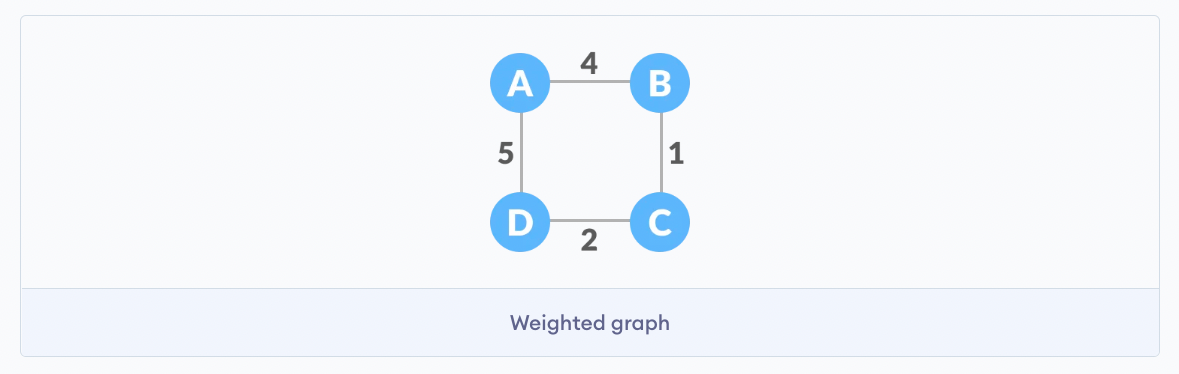
\includegraphics[scale=0.4]{minimum-spanning-tree-1}
\caption{\footnotesize{A Weighted Undirected Graph}}
\captionsetup{aboveskip=0pt,font=it}
\end{figure}
\bigskip

\begin{figure}[hp]
\centering
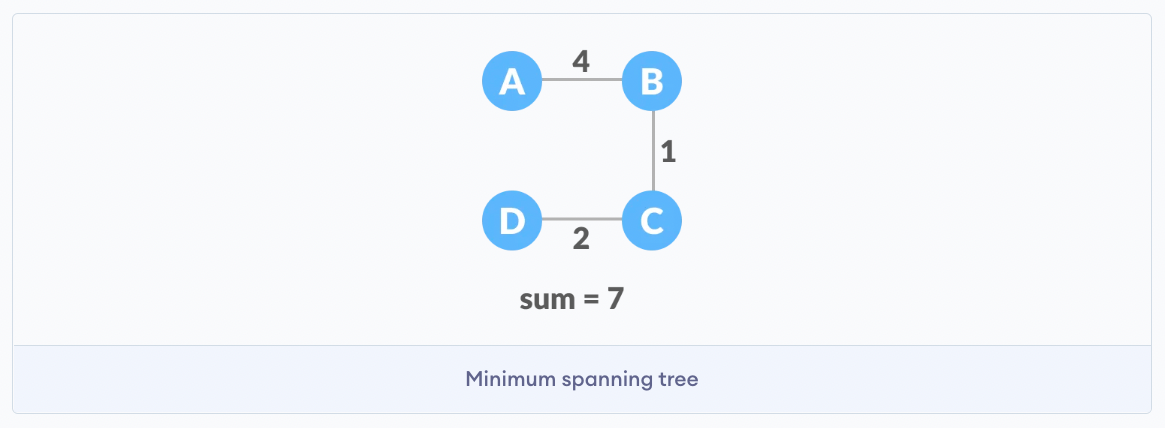
\includegraphics[scale=0.4]{minimum-spanning-tree-2}
\caption{\footnotesize{Minimum Spanning Tree for the above Graph, in this case 7 (4 + 1 + 2)}}
\captionsetup{aboveskip=0pt,font=it}
\end{figure}
\bigskip

In our testing script, we again set \(V\) to the number of vertices on a side with the total number of vertices being \(V^2\). Furthermore, we define \(E\) as edge, where \(E = V - 1\). Each \(E\) connects \(V[i]\) with \(V[i+1]\), where \(i\) is the index of \(E\).

We then run the algorithm on the graph and measure its runtime. The algorithm finds and traverses through the minimum spanning tree of our graph. The average runtime complexity is \(O(E\cdot\ Log(E))\) where \(E\) is the the total number of edges in the graph. The size of the input datasets (number of edges) are 400000, 1000000 and 2100000 respectively. Thus, the total runtime for our Kruskal’s Algorithm benchmarking test is:

\[ O(E\cdot\ Log(E))\ where\ E = V - 1, V \in \{400000, 1000000, 2100000\} \]
\[ =O(E\cdot\ Log(E))\ where\ E \in \{399999, 999999, 2099999\} \]

\bigskip
\textbf{{\normalsize Chapter 4.10.4 Prim's Algorithm}}

Finally, we benchmark Prim's Algorithm. Just like Kruskal’s Algorithm, Prim's Algorithm is a greedy, minimum spanning tree algorithm [112]. However, unlike Kruskal’s Algorithm, Prim's Algorithm selects the root vertex upon execution and gradually expand outwards until it has traversed the whole graph [113]. In our benchmarking test, we set \(V\) to be the number of vertices on a side with the total number of vertices being \(V^2\). After that, just like Floyd’s Algorithm, we set \(E\) to be the number of all edges in the graph where \(V = E\). Each edges have a 50\% chance of having an zero (0) weight. When this occurs, we consider the pair of vertices not connected. For connected edges, each has a weight distance randomly generated between 1 and 99.

We then run the algorithm on the graph and measure its runtime. Prim's Algorithm finds and traverses through the minimum spanning tree of our graph. Its average runtime complexity is \(O(E\cdot\ Log(V))\) where \(V\) is the number of vertices in the graph and \(E\) is the number of edges in the graph. The size of the input datasets (number of edges) are 400, 550 and 680 respectively. Thus, the total runtime for our Prim’s Algorithm benchmarking test is:

\[ O(E\cdot\ Log(V))\ where\ E, V \in \{400, 550, 680\} \]

\bigskip
\textbf{{\Large Chapter 4.11 The Next Episode}}

After conducting both stages of out experiment, we present our findings in the results section. Also in the next section, we will analyse on our results and present interesting and unexpected findings.
\chapter{Results} \label{chap:results}

\bigskip
\section{The Unexpected Results}

In the first stage of the experiment, after comparing the two frameworks running sorting algorithms, we discovered that Flask has a better performance than Spin in contrast to our initial hypothesis. Therefore, we decided to expand on the algorithm comparison and further introduce 4 more minimum distance and spanning tree algorithms. They are Dijkstra' Algorithm, Floyd's Algorithm, Kruskal's Algorithm and Prim's Algorithm.

As shown in the figure below, in both stages of the experiment, the Flask framework consistently outpaced the WebAssembly Spin framework with some algorithms benchmarking more than 100\% faster. In this section, we will dive deeper into the data and analyse the reason behind such inconsistent behaviour.

In the first stage of the experiment, we compared the runtime performance across 3 platforms: native in the local environment, online production via Flask and online production via Spin. The native environment is marked with the blue bar, Flask with orange and Spin with grey. Comparing the runtime performance between Flask and Spin, we clearly notice a visible performance gap. Across \textbf{18} benchmarking algorithms running \textbf{54} tests in total, only \textbf{1} algorithm across \textbf{3} tests, or \textbf{5.6} percent of the times where Spin outperformed Flask \textbf{(Bucket Sort)}. In this case, the runtime for Spin is \textbf{2.28s, 6.07s, 10.5s} for small, medium and large input sizes, respectively. This was faster than Flask's runtime, which was \textbf{2.38s, 6.82s and 11.95s} on average across running the algorithm \textbf{5} times.

Here is the runtime comparison across all 18 benchmarking algorithms (average of 5 runs):

\newpage
\bigskip
\begin{figure}[hp]
\centering
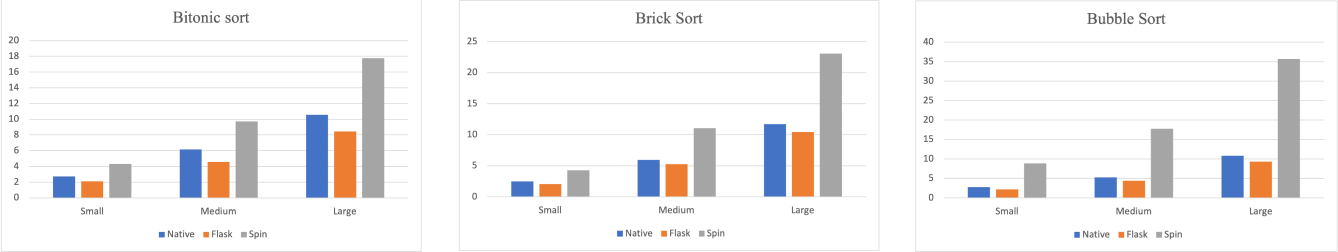
\includegraphics[scale=0.33]{sort1}
\caption{\footnotesize{Benchmark on Bitonic Sort, Brick Sort and Bubble Sort}}
\captionsetup{aboveskip=0pt,font=it}
\end{figure}
\bigskip

\bigskip
\begin{figure}[hp]
\centering
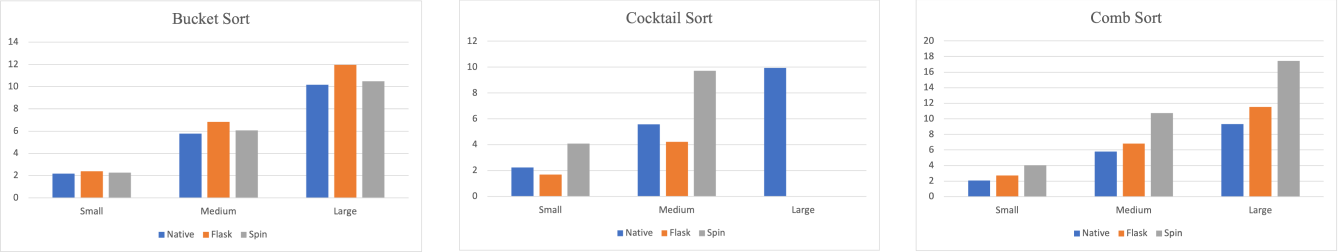
\includegraphics[scale=0.33]{sort2}
\caption{\footnotesize{Benchmark on Bucket Sort, Cocktail Sort and Comb Sort}}
\captionsetup{aboveskip=0pt,font=it}
\end{figure}
\bigskip

\bigskip
\begin{figure}[hp]
\centering
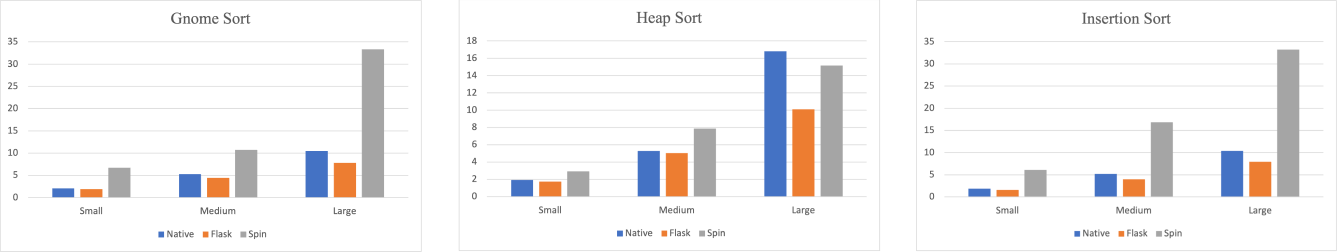
\includegraphics[scale=0.33]{sort3}
\caption{\footnotesize{Benchmark on Gnome Sort, Heap Sort and Insertion Sort}}
\captionsetup{aboveskip=0pt,font=it}
\end{figure}
\bigskip

\bigskip
\begin{figure}[hp]
\centering
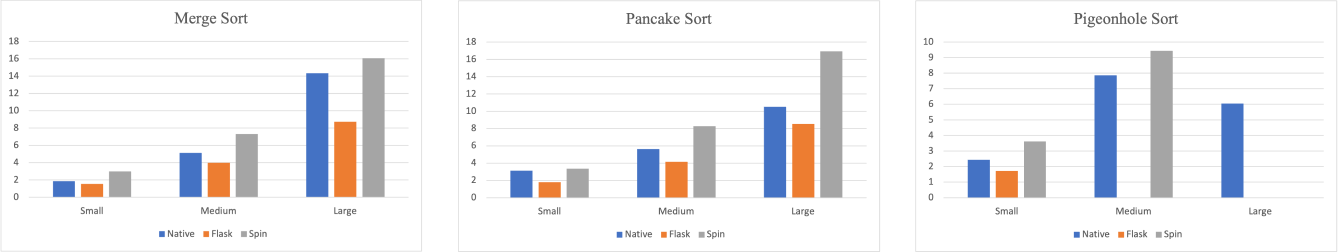
\includegraphics[scale=0.33]{sort4}
\caption{\footnotesize{Benchmark on Merge Sort, Pancake Sort and Pigeonhole Sort}}
\captionsetup{aboveskip=0pt,font=it}
\end{figure}
\bigskip

\newpage
\bigskip
\begin{figure}[hp]
\centering
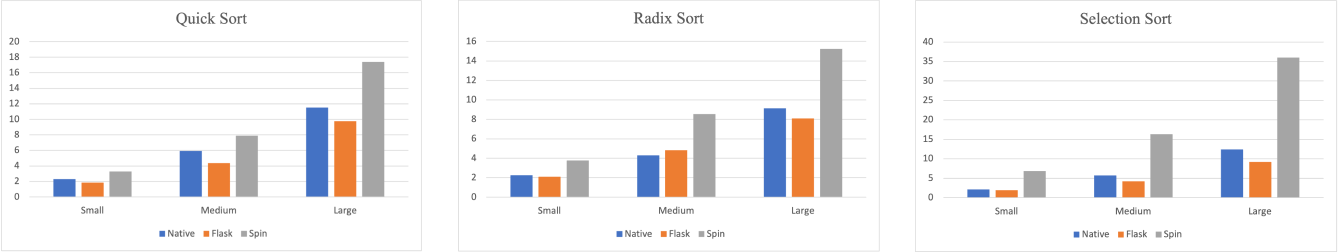
\includegraphics[scale=0.33]{sort5}
\caption{\footnotesize{Benchmark on Quick Sort, Radix Sort and Selection Sort}}
\captionsetup{aboveskip=0pt,font=it}
\end{figure}
\bigskip

\bigskip
\begin{figure}[hp]
\centering
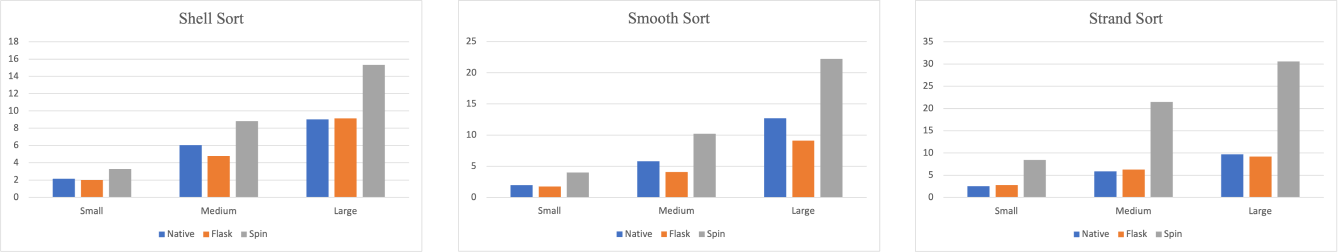
\includegraphics[scale=0.33]{sort6}
\caption{\footnotesize{Benchmark on Shell Sort, Smooth Sort and Strand Sort}}
\captionsetup{aboveskip=0pt,font=it}
\end{figure}
\bigskip

\bigskip
\section{The Outlier}

The outlier here is Bucket Sort. Therefore it is appropriate to list out some of its properties and to form a few hypotheses on the reason behind Spin running faster than Flask executing this algorithm.

We first look at the data input sizes for Bucket Sort with the input array length being \textbf{35000, 55000 and 70000} for small, medium and large, respectively, with the average input length of \textbf{53333}. We do not see this number as an outlier, as other algorithms have a far greater or far smaller average input size. For example, Pigeonhole Sort has an average input array size of \textbf{11666666}, and Brick Sort has an average input array size of \textbf{800}. According to the graph below, Bucket Sort's average array input size is somewhere in the middle across all sorting algorithms.

However, if we remove the \textbf{top two} algorithms with the largest average input array size, we will see a far more average graph with around half \textbf{(7)} of the algorithms having an average input size between \textbf{200000} and \textbf{1000000} (second graph below).

\newpage
\bigskip
\begin{figure}[hp]
\centering
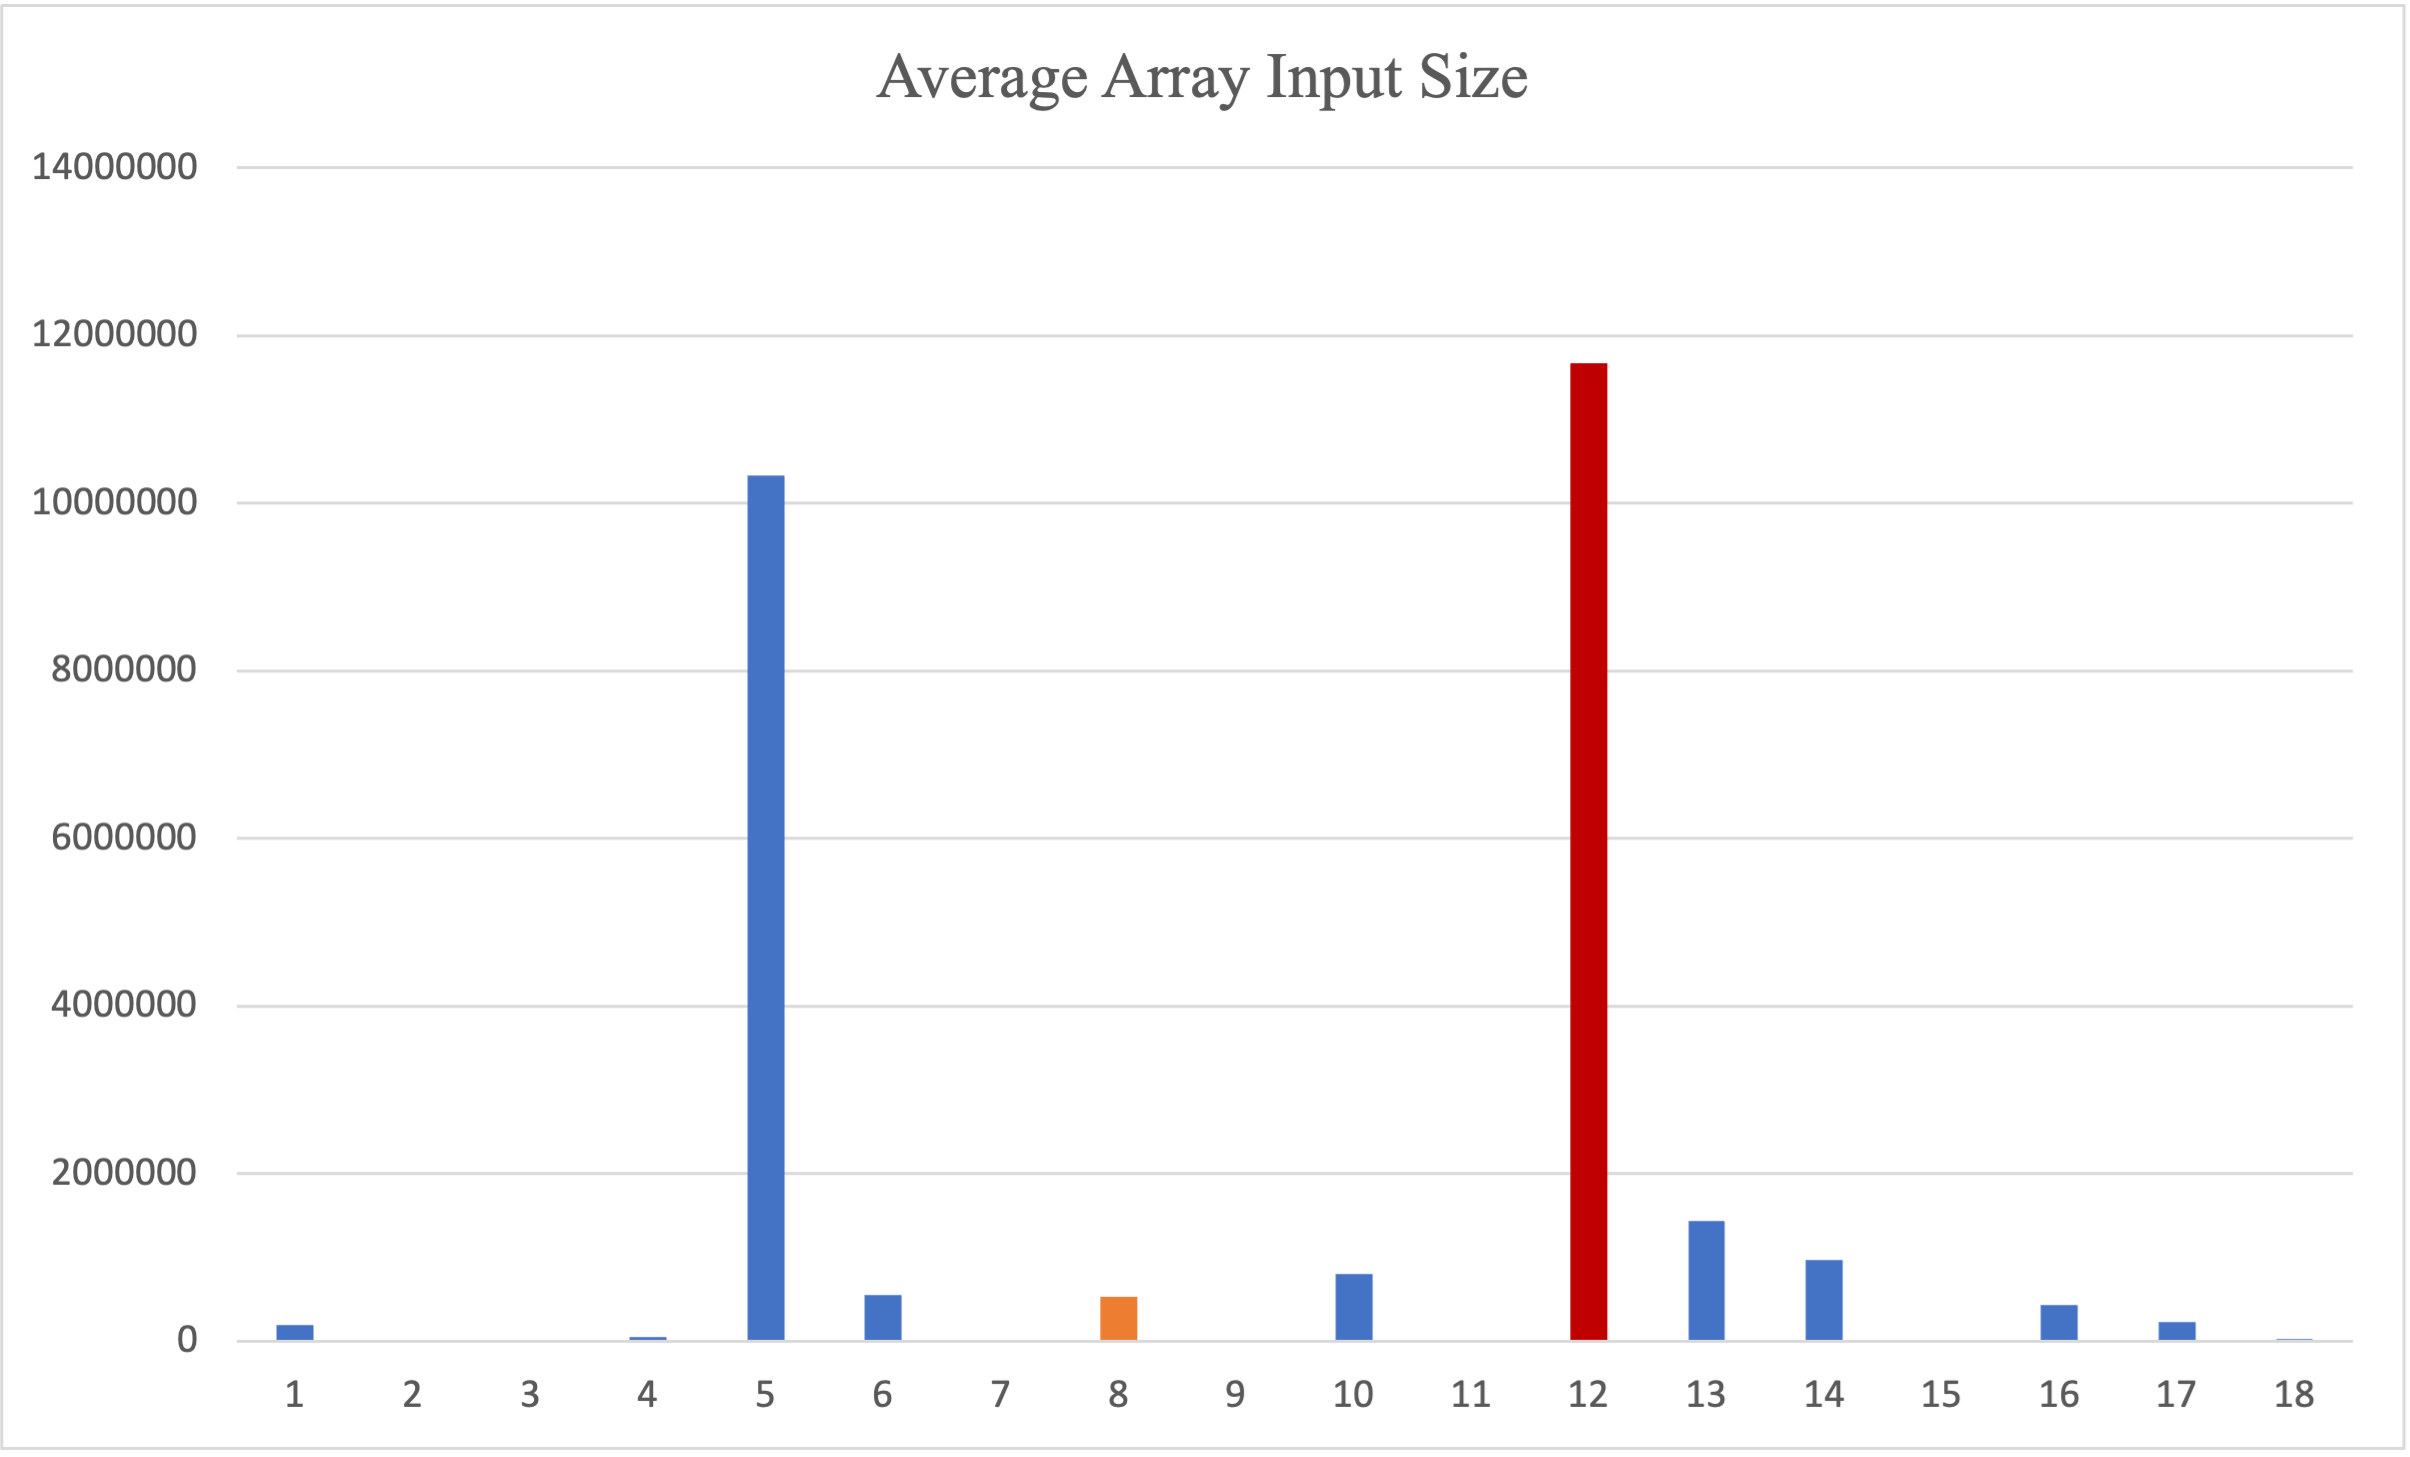
\includegraphics[scale=0.7]{average-sorting-size}
\caption{\footnotesize{Average array input size for all algorithms, green is Brick Sort (non-visible), orange is Bucket Sort, and red is Pigeonhole Sort}}
\captionsetup{aboveskip=0pt,font=it}
\end{figure}
\bigskip

\bigskip
\begin{figure}[hp]
\centering
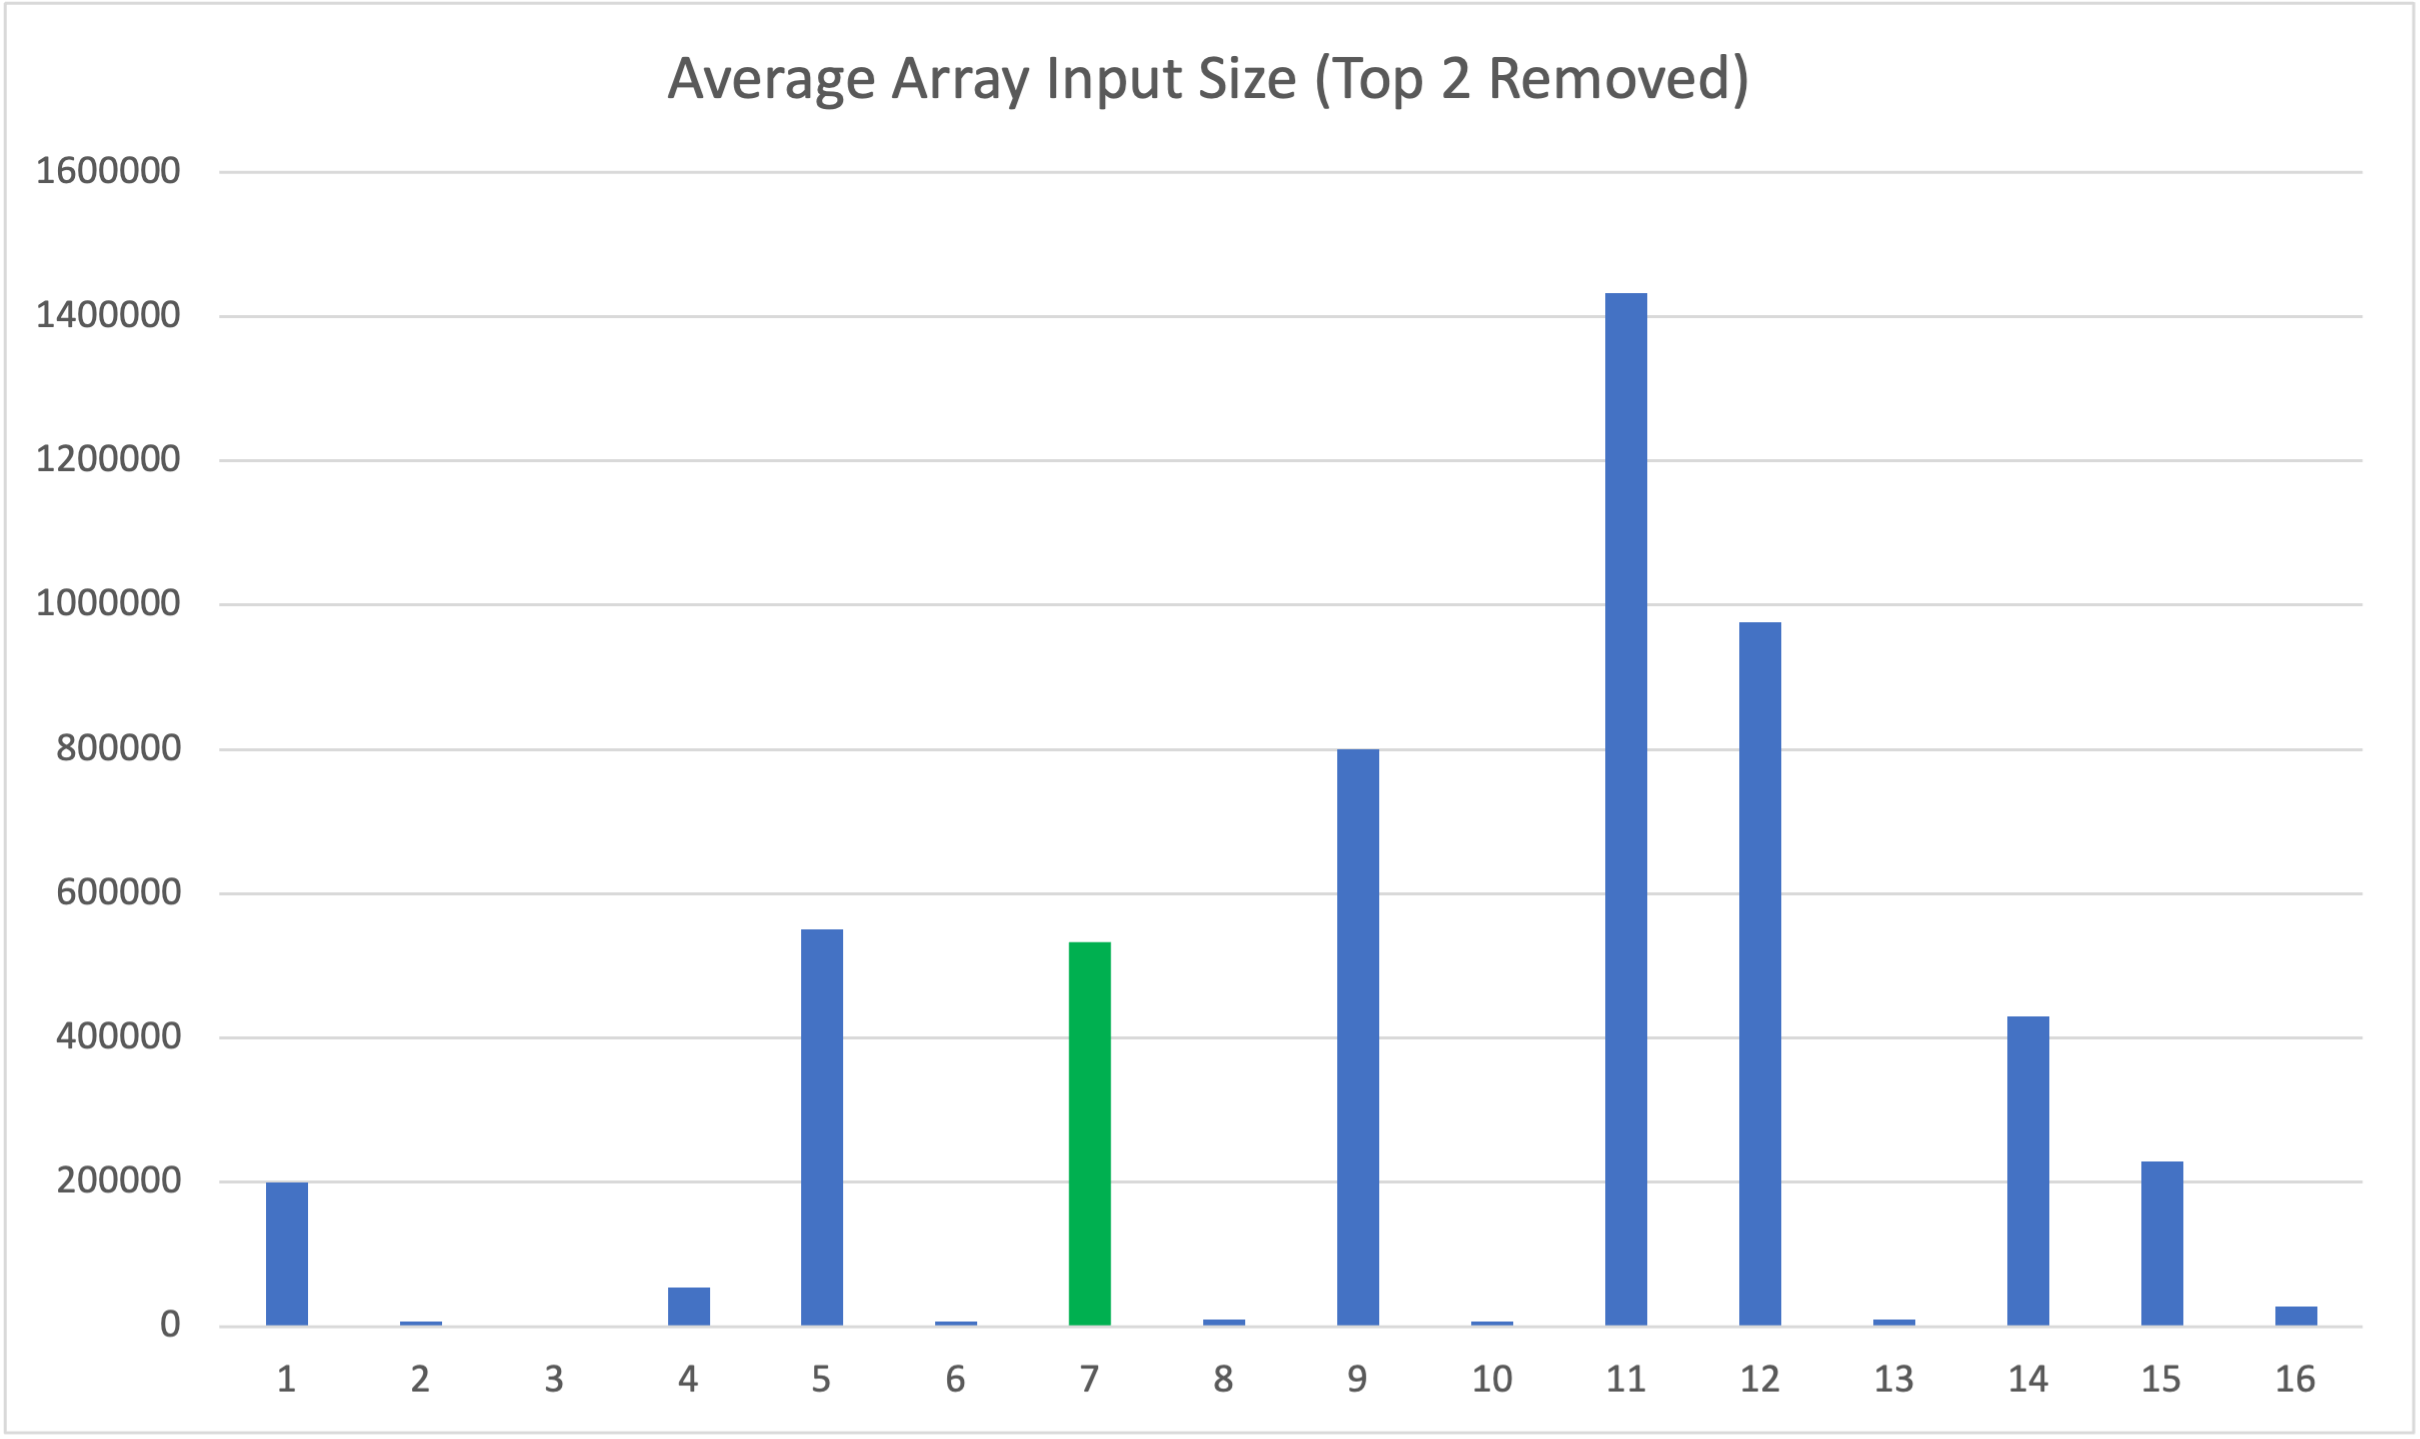
\includegraphics[scale=0.7]{average-sorting-size-2-removed}
\caption{\footnotesize{Average array input size for our sorting algorithm collection with top 2 removed}}
\captionsetup{aboveskip=0pt,font=it}
\end{figure}
\bigskip

We conclude that the input size is not a factor here; therefore, we continue to explore and find out the potential factor behind the performance inconsistency on both frameworks for Bucket Sort.

We then move on to the space complexity for Bucket Sort. As well as addressing the concept behind the algorithm. The space complexity for Bucket Sort is \(n + k\) on average, with the worst space complexity being \(\theta(n\ \cdot\ k)\), where \(n\) is the number of elements in the array and \(k\) is the number of "buckets" used during the sorting process. After adding all elements to \(k\) number of buckets, it will then sort each \(k\) bucket individually with Insertion Sort, which has a space complexity of \(O(1)\).

\bigskip
\begin{figure}[hp]
\centering
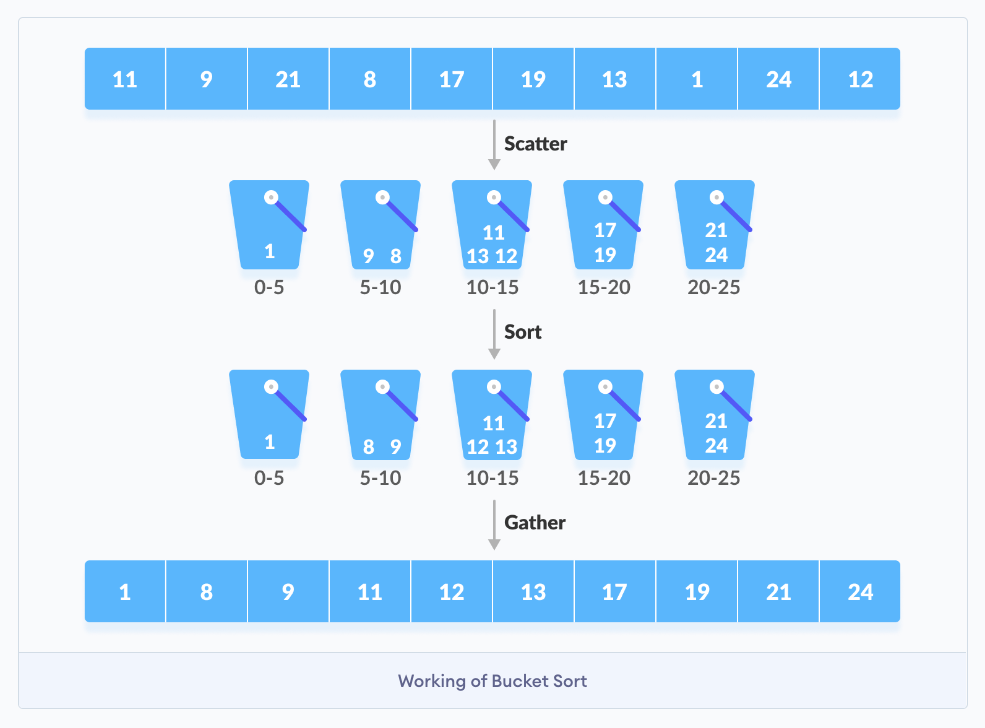
\includegraphics[scale=0.4]{bucket-proz}
\caption{\footnotesize{Working of Bucket Sort \cite{res1}}}
\captionsetup{aboveskip=0pt,font=it}
\end{figure}
\bigskip

From the above figure, we presented the workflow concept for Bucket Sort. At the same time, we recognise that the number of buckets \(k\) can be very different based on the input array. This adds inconsistency to its space complexity, and because of the "bucket" concept used in the algorithm, it uses more memory than any other algorithms in our collection.

Thus, we believe this to be the reason why the Flask framework performs worse than the Spin framework when running Bucket Sort on the input arrays. Especially when running on resource-constraint devices such as the Amazon t3 micro machine, which we introduced in the previous section. On the other hand, WebAssembly has the excellent ability to manage memory usage, and it has clearly shown in this case. Also, note that running this algorithm natively has better performance due to the machine it's running on (2017 MacBook Pro) having a far superior CPU and larger memory.

\bigskip
\section{The Elephant in the Room}

\subsection{Flask vs. Spin}

Except for Bucket Sort, the Flask framework outperformed Spin in 17 out of 18 sorting benchmarks. It was a bit of a surprise when we first recorded the result, and therefore, we ran all experiments 5 times and took the average runtime just to be absolutely sure that the results we were getting from the experiment were consistent. On average, for 17 out of 18 algorithms where Flask outperformed Spin, it ran faster by \textbf{139.212\%} with the lowest runtime increase being \textbf{36.992\%} and the highest being \textbf{309.957\%}.

\bigskip
\begin{figure}[hp]
\centering
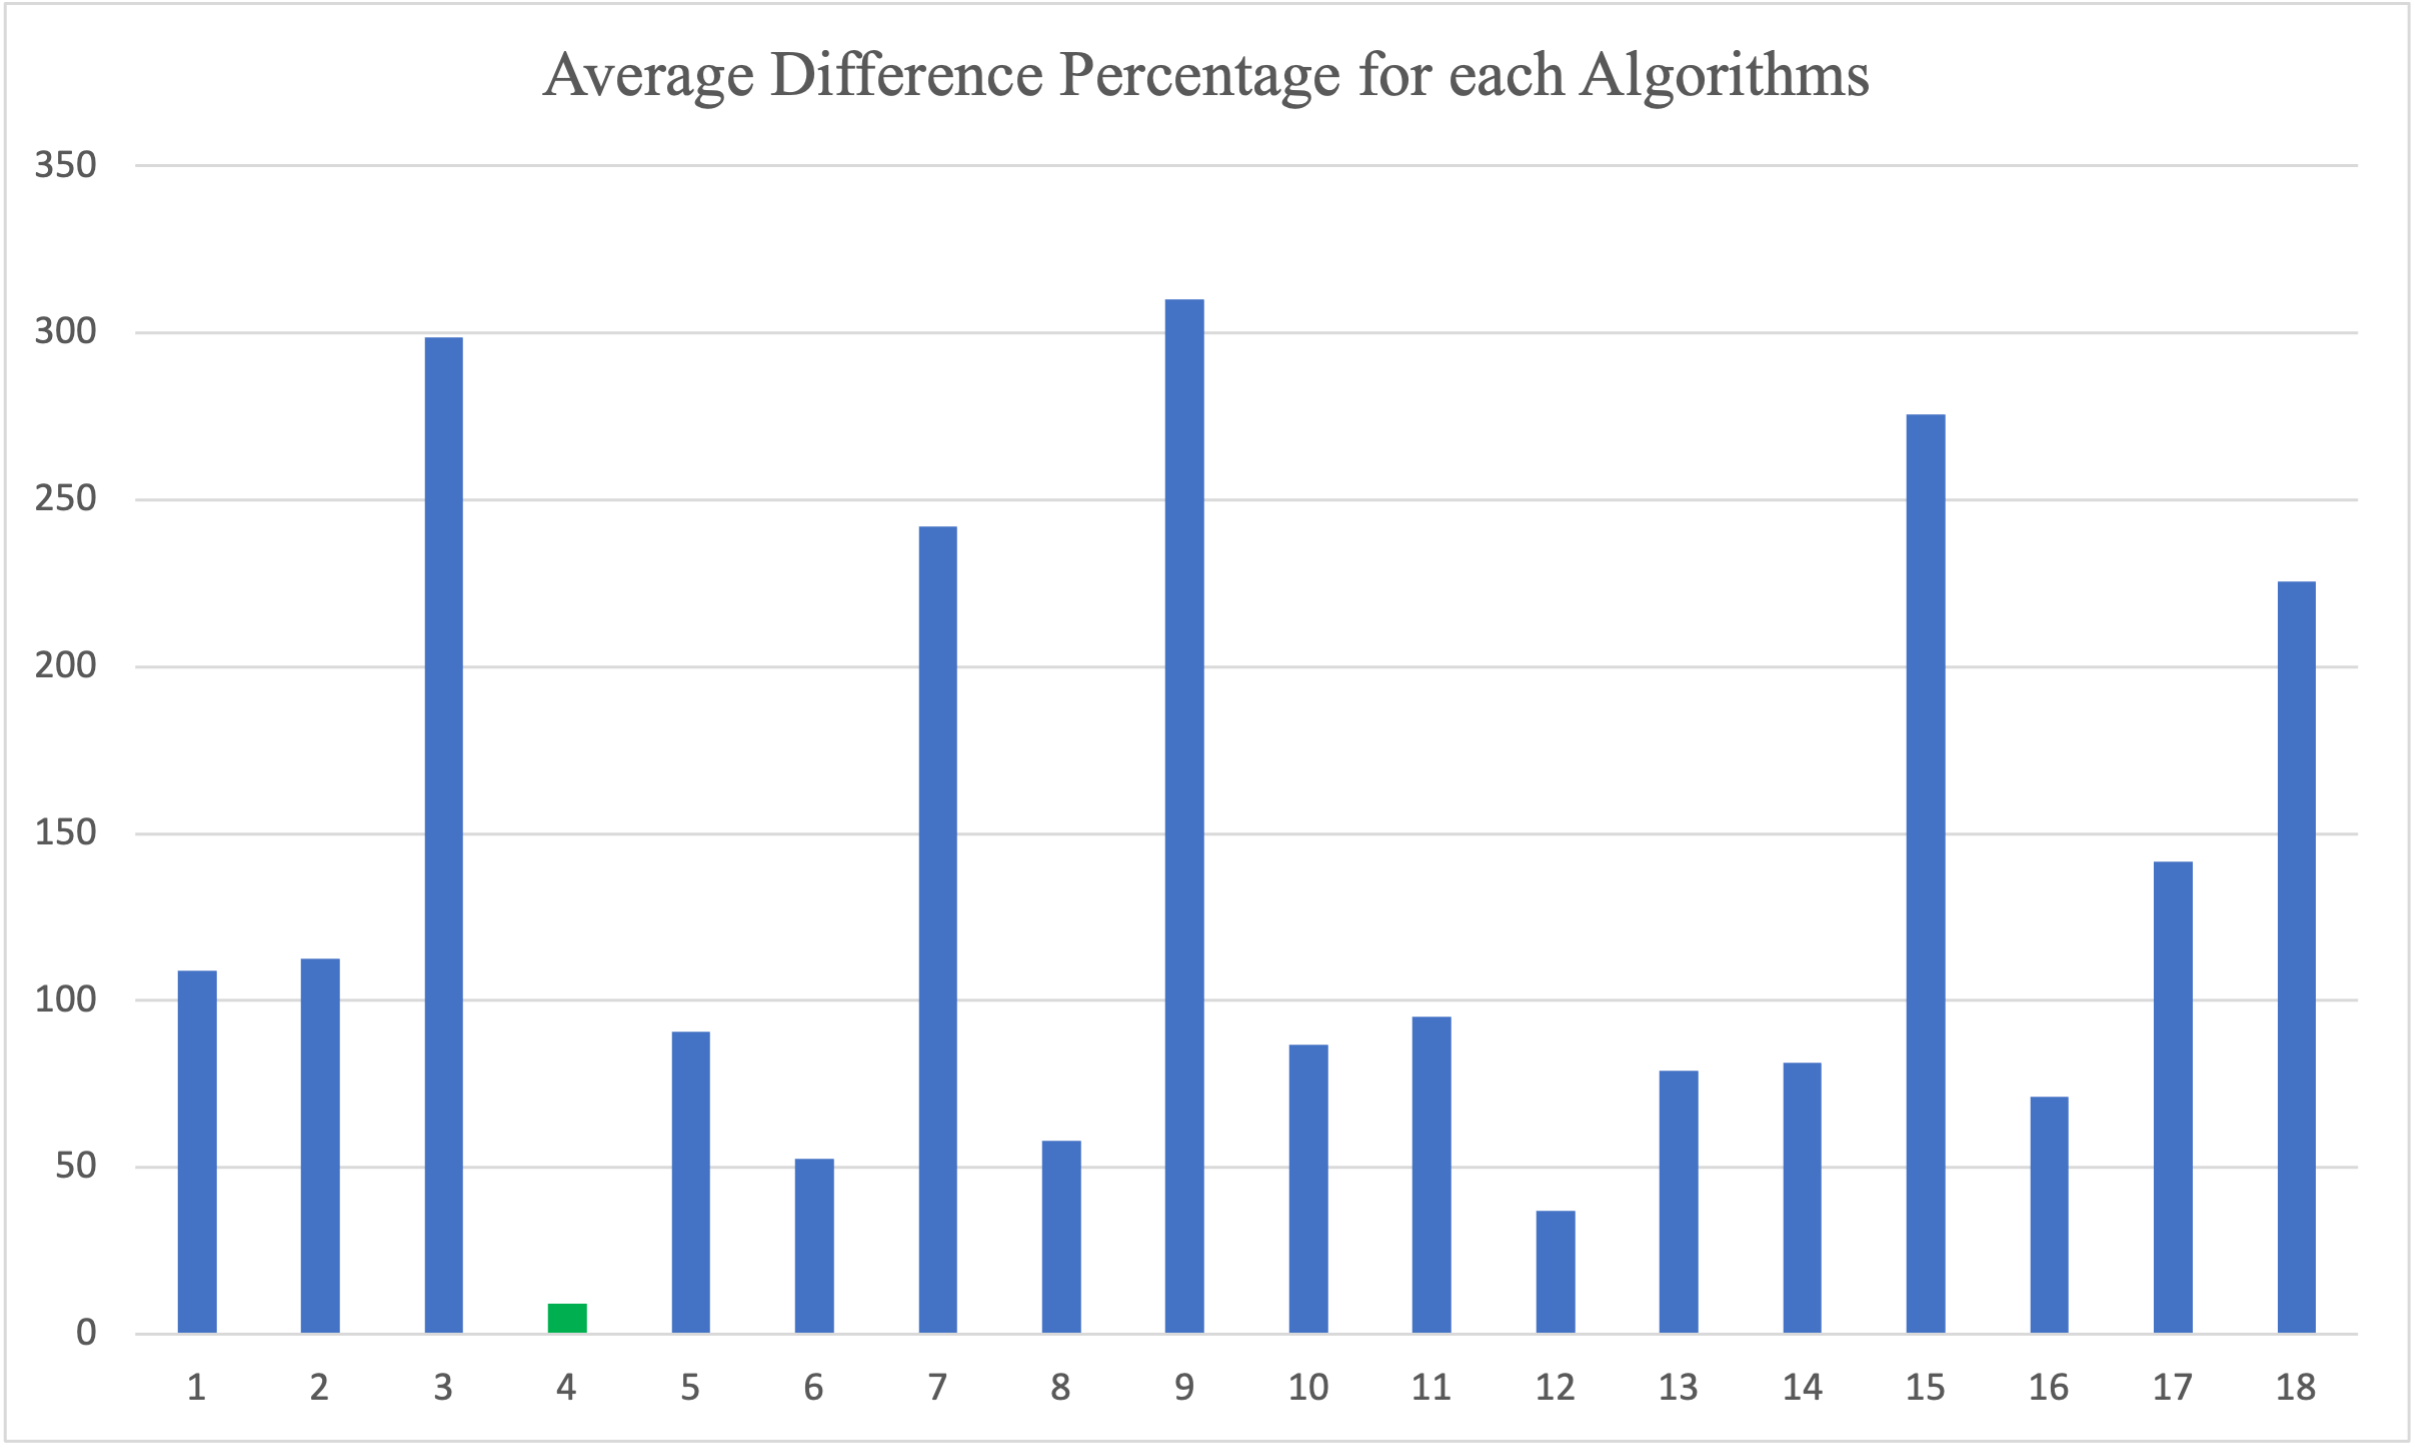
\includegraphics[scale=0.7]{avg-sorting-per}
\caption{\footnotesize{Average performance difference between Flask and Spin, Bucket Sort where Spin outperformed Flask is marked green}}
\captionsetup{aboveskip=0pt,font=it}
\end{figure}
\bigskip

We kept exploring further, and we found that there could be a correlation between the array input size with the average algorithm performance difference. The algorithms with the highest performance differences are \textbf{Brick Sort}, \textbf{Gnome Sort}, \textbf{Insertion Sort}, \textbf{Selection Sort} and \textbf{Strand Sort}. At the same time, they also have some of the smallest array input sizes. In contrast, the \textbf{mean} and the \textbf{medium} for the algorithm performance difference are \textbf{329685.19} and \textbf{126666.5}, respectively. \textbf{Brick Sort} has an average array input size of \textbf{800}, which is way lower than both the mean and the medium. This is also the case with all 4 other algorithms. In fact, \textbf{Brick Sort} and \textbf{Gnome Sort} have the two lowest array input size out of all \textbf{18} algorithms \textbf{(800 and 6500)}, while \textbf{Selection Sort} has the \textbf{fifth} lowest array input size \textbf{(9833)}, \textbf{Insertion Sort} \textbf{sixth} \textbf{(10000)}, and \textbf{Strand Sort}, \textbf{seventh} \textbf{(28333)}.

\bigskip
\begin{figure}[hp]
\centering
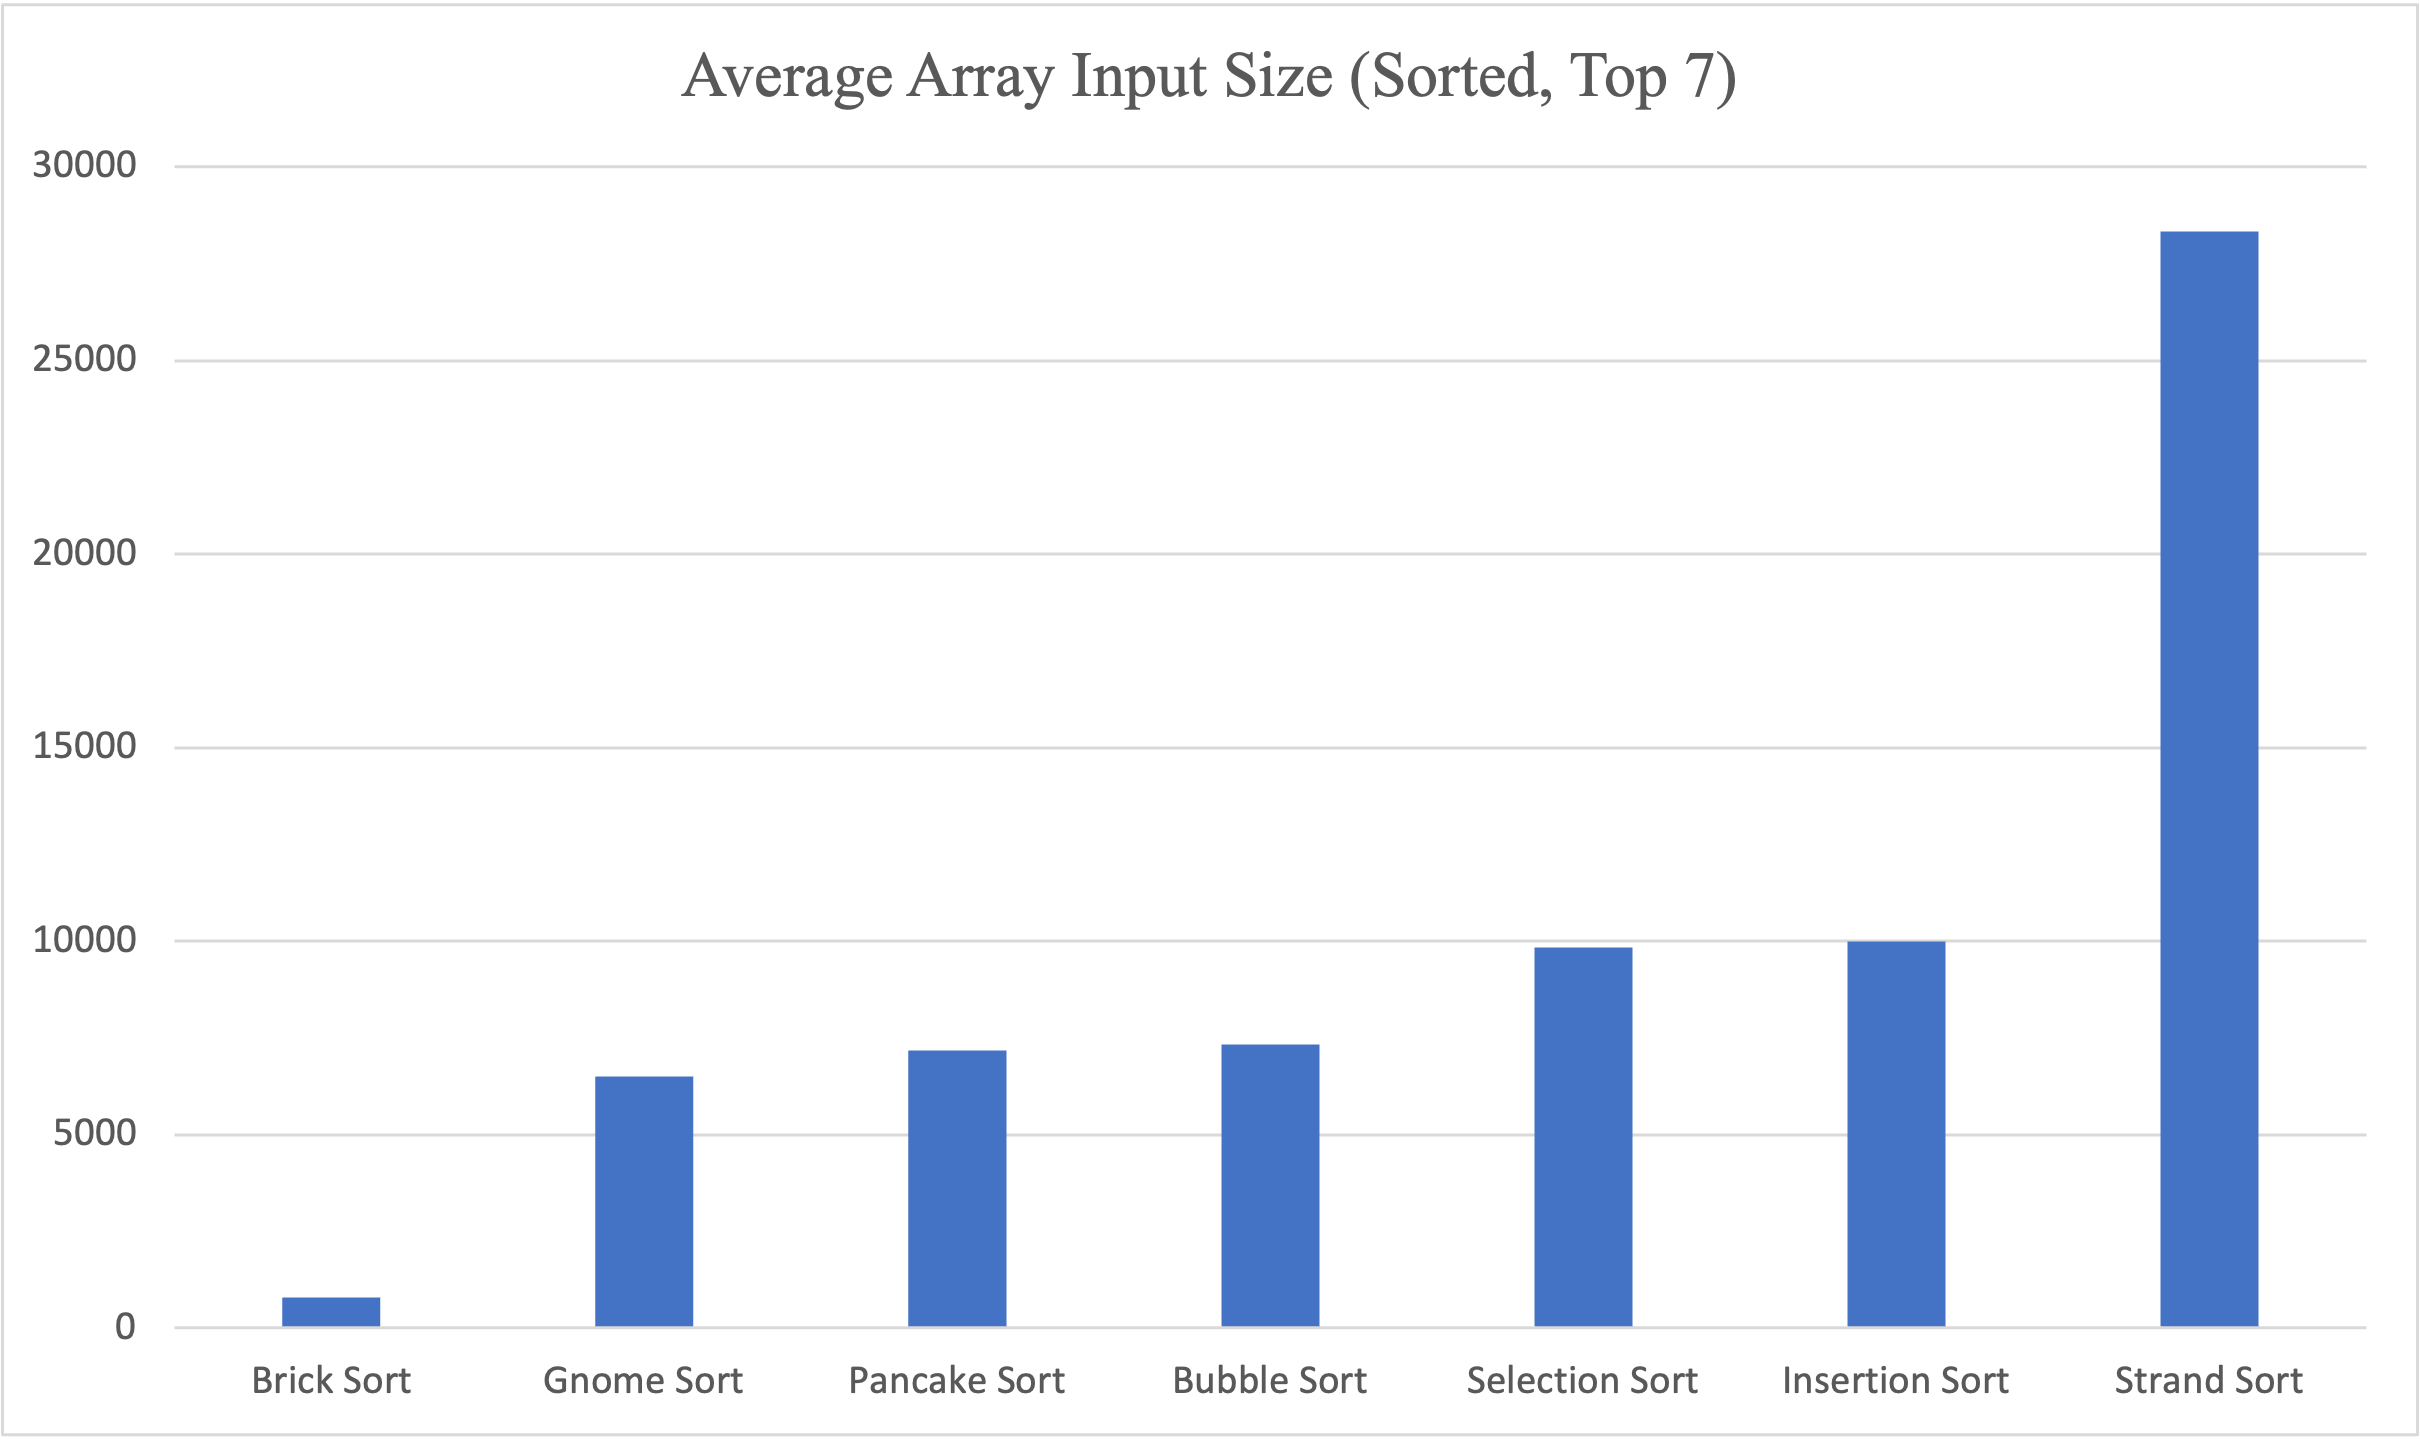
\includegraphics[scale=0.7]{avg-sorting-per-sorted-7}
\caption{\footnotesize{Average array input size (Sorted from lowest to highest, Top 7)}}
\captionsetup{aboveskip=0pt,font=it}
\end{figure}
\bigskip

\subsection{Native Environment vs. Flask}

We also noticed that the Flask framework outperformed the Native Environment from time to time. Across \textbf{18} benchmarks and \textbf{51} valid tests where both Native and Flask runtime data were recorded successfully, Native only outperformed Flask \textbf{10} times, or \textbf{19.6\%} of time.

Ahead of the experiment, we believe benchmarks running on a native environment will perform best since it has little overhead as well as more CPU and memory resources than running in a cloud or edge environment. However, we believe this inconsistency is due to the continuous development, optimisation and integration with Python on the Flask framework, which was initially released back in 2010.

\bigskip
\section{Further Exploring with Standard Deviation}

As stated above, we run each benchmark \textbf{5} times to ensure the result data is consistent. We calculate the standard deviation for \textbf{5} benchmarks \textbf{(Quick Sort, Merge Sort, Selection Sort, Insertion Sort and Bubble Sort)} to ensure runtime from each iteration does not spread out too much.

\bigskip
\begin{table}[h!]
\centering
\begin{tabular}{||c c c c||} 
\hline
Name & Standard Deviation ($\sigma$) & Confidence Interval & 95\% Confidence Interval \\ [1ex] 
\hline\hline
 & & & \\
Quick Sort (S) & 0.16 & 0.071 & 1.8424 ±0.14 (±7.62\%) \\
 & & & \\
Quick Sort (M) & 0.17 & 0.075 & 4.3692 ±0.146 (±3.35\%) \\
 & & & \\
Quick Sort (L) & 0.436 & 0.195 & 9.7668 ±0.382 (±3.91\%) \\
 & & & \\
Merge Sort (S) & 0.045 & 0.02 & 1.5396 ±0.0395 (±2.56\%) \\
 & & & \\
Merge Sort (M) & 0.13 & 0.058 & 3.9864 ±0.114 (±2.86\%) \\
 & & & \\
Merge Sort (L) & 0.416 & 0.186 & 8.7294 ±0.365 (±4.18\%) \\
 & & & \\
Selection Sort (S) & 0.154 & 0.069 & 1.9406 ±0.135 (±6.97\%) \\
 & & & \\
Selection Sort (M) & 0.188 & 0.084 & 4.2406 ±0.165 (±3.88\%) \\
 & & & \\
Selection Sort (L) & 0.144 & 0.064 & 9.2008 ±0.126 (±1.37\%) \\
 & & & \\
Insertion Sort (S) & 0.143 & 0.064 & 1.5734 ±0.125 (±7.97\%) \\
 & & & \\
Insertion Sort (M) & 0.264 & 0.118 & 3.9772 ±0.231 (±5.81\%) \\
 & & & \\
Insertion Sort (L) & 0.437 & 0.195 & 7.9312 ±0.383 (±4.83\%) \\
 & & & \\
Bubble Sort (S) & 0.021 & 0.009 & 2.167 ±0.0187 (±0.86\%) \\
 & & & \\
Bubble Sort (M) & 0.149 & 0.067 & 4.4062 ±0.13 (±2.96\%) \\
 & & & \\
Bubble Sort (L) & 0.605 & 0.27 & 9.2836 ±0.53 (±5.71\%) \\ [1ex]
\hline
\end{tabular}
\caption{Standard deviation for Flask framework}
\label{table:time_complexity_2}
\end{table}
\bigskip

\bigskip
\begin{table}[h!]
\centering
\begin{tabular}{||c c c c||} 
\hline
Name & Standard Deviation ($\sigma$) & Confidence Interval & 95\% Confidence Interval \\ [1ex] 
\hline\hline
 & & & \\
Quick Sort (S) & 0.111 & 0.05 & 3.2788 ±0.0975 (±2.97\%) \\
 & & & \\
Quick Sort (M) & 0.214 & 0.075 & 0.096 ±0.187 (±2.37\%) \\
 & & & \\
Quick Sort (L) & 0.5 & 0.222 & 17.3986 ±0.436 (±2.50\%) \\
 & & & \\
Merge Sort (S) & 0.253 & 0.113 & 2.9772 ±0.221 (±7.43\%) \\
 & & & \\
Merge Sort (M) & 0.314 & 0.14 & 7.3058 ±0.275 (±3.77\%) \\
 & & & \\
Merge Sort (L) & 0.9 & 0.402 & 16.0678 ±0.789 (±4.91\%) \\
 & & & \\
Selection Sort (S) & 0.307 & 0.137 & 6.8086 ±0.269 (±3.96\%) \\
 & & & \\
Selection Sort (M) & 0.532 & 0.238 & 16.3238 ±0.466 (±2.86\%) \\
 & & & \\
Selection Sort (L) & 0.759 & 0.339 & 35.981 ±0.665 (±1.85\%) \\
 & & & \\
Insertion Sort (S) & 0.069 & 0.03 & 6.096 ±0.0603 (±0.99\%) \\
 & & & \\
Insertion Sort (M) & 0.306 & 0.137 & 16.8586 ±0.268 (±1.59\%) \\
 & & & \\
Insertion Sort (L) & 0.909 & 0.407 & 33.196 ±0.797 (±2.40\%) \\
 & & & \\
Bubble Sort (S) & 0.343 & 0.154 & 8.8656 ±0.301 (±3.39\%) \\
 & & & \\
Bubble Sort (M) & 0.335 & 0.15 & 17.7418 ±0.294 (±1.66\%) \\
 & & & \\
Bubble Sort (L) & 0.954 & 0.427 & 35.6476 ±0.837 (±2.35\%) \\ [1ex]
\hline
\end{tabular}
\caption{Standard deviation for Spin framework}
\label{table:time_complexity_2}
\end{table}
\bigskip

We discovered a few interesting things in the above analysis for the standard deviation. First, overall the standard deviation for all benchmarking algorithms with all 3 data input sizes is relatively small. This means the runtime data we get from running the benchmark algorithms each time are fairly consistent and do not spread out too much. Thus, we can be sure that we are confident with the data we analysed using the average runtime data calculated in the earlier section.

The second thing we found is that for both frameworks, we tend to get a larger number of standard deviations than the input data. For example, the average standard deviation for \textbf{small} array input size is \textbf{0.105} for Flask and \textbf{0.217} for Spin. In contrast, the average standard deviation for \textbf{large} array input size is \textbf{0.408} for Flask and \textbf{0.804} for Spin, which is \textbf{3.9 times} and \textbf{3.72 times} greater than their small data input counterpart respectively. This means that the result data spreads wider and less consistent the larger the input data is. This is also an interesting phenomenon that we believe is worthy of further research.

\bigskip
\section{Shortest Path and Minimum Spanning Tree Algorithm Analysis}

The second stage of our experiment is benchmarking an extra \textbf{4} Shortest Path and Minimum Spanning Tree Algorithms. They are \textbf{Dijkstra's algorithm}, \textbf{Floyd–Warshall algorithm}, \textbf{Kruskal's algorithm} and \textbf{Prim's algorithm}.

\subsection{Performances between Flask and Spin}

For all \textbf{4} benchmarking algorithms in the second stage \textbf{(10 valid tests)}, Flask outperformed Spin on every single one of them by an average of \textbf{107.571\%}, with the lowest runtime increase being \textbf{30.224\%} and the highest being \textbf{151.368\%}. On the other hand, the average runtime increase with the \textbf{small} data input size is \textbf{290.322\%}, the \textbf{medium}: \textbf{106.057\%} and the \textbf{large} is \textbf{138.753\%}. With the knowledge from the first experiment, we are not surprised by the results we got from the shortest path and minimum spanning tree algorithms.

Here are the results from stage 2 of the experiment:

\bigskip
\begin{figure}[hp]
\centering
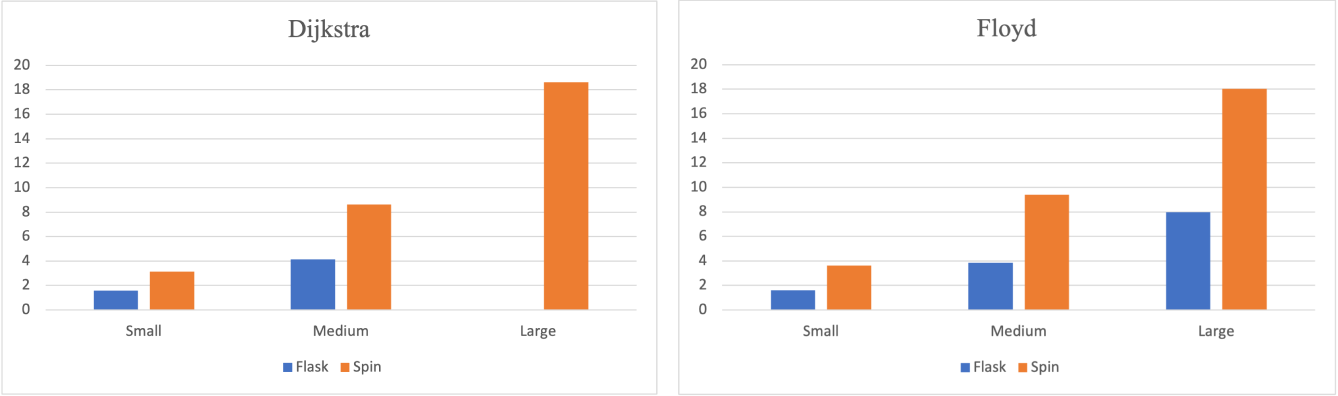
\includegraphics[scale=0.33]{images/other1}
\caption{\footnotesize{Benchmark on Dijkstra and Floyd–Warshall}}
\captionsetup{aboveskip=0pt,font=it}
\end{figure}
\bigskip

\newpage
\bigskip
\begin{figure}[hp]
\centering
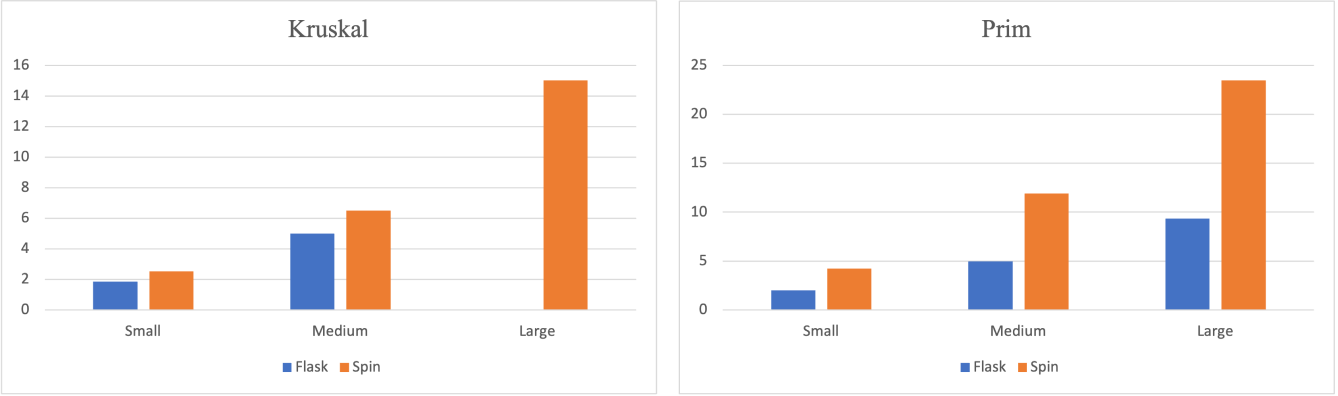
\includegraphics[scale=0.33]{images/other2}
\caption{\footnotesize{Benchmark on Kruskal and Prim}}
\captionsetup{aboveskip=0pt,font=it}
\end{figure}
\bigskip


\subsection{The case of Kruskal's Algorithm}

We further look at the average speed-up percentage per algorithm. For Dijkstra's algorithm, Flask outperformed Spin by \textbf{103.784\%} on average. For Floyd–Warshall, it was \textbf{132.923\%}. Then, Kruskal, \textbf{33.132\%} on average and lastly, Flask outperformed Spin by \textbf{134.369\%} on average running Prim's algorithm.

In the case of Kruskal's algorithm, we discovered that the average speed-up percentage is lower than the other 3 algorithms. In fact, Kruskal's algorithm is the only benchmarking algorithm in our collection where the average speed-up percentage is below 100\%. It is also below the average speed-up percentage across all tests by \textbf{224.679\%}. Within \textbf{8} tests performed across Dijkstra, Floyd and Prim, only \textbf{1} test where the average speed-up rate is below 100 \textbf{(Dijkstra's algorithm with small input data)}.

\newpage
\begin{figure}[hp]
\centering
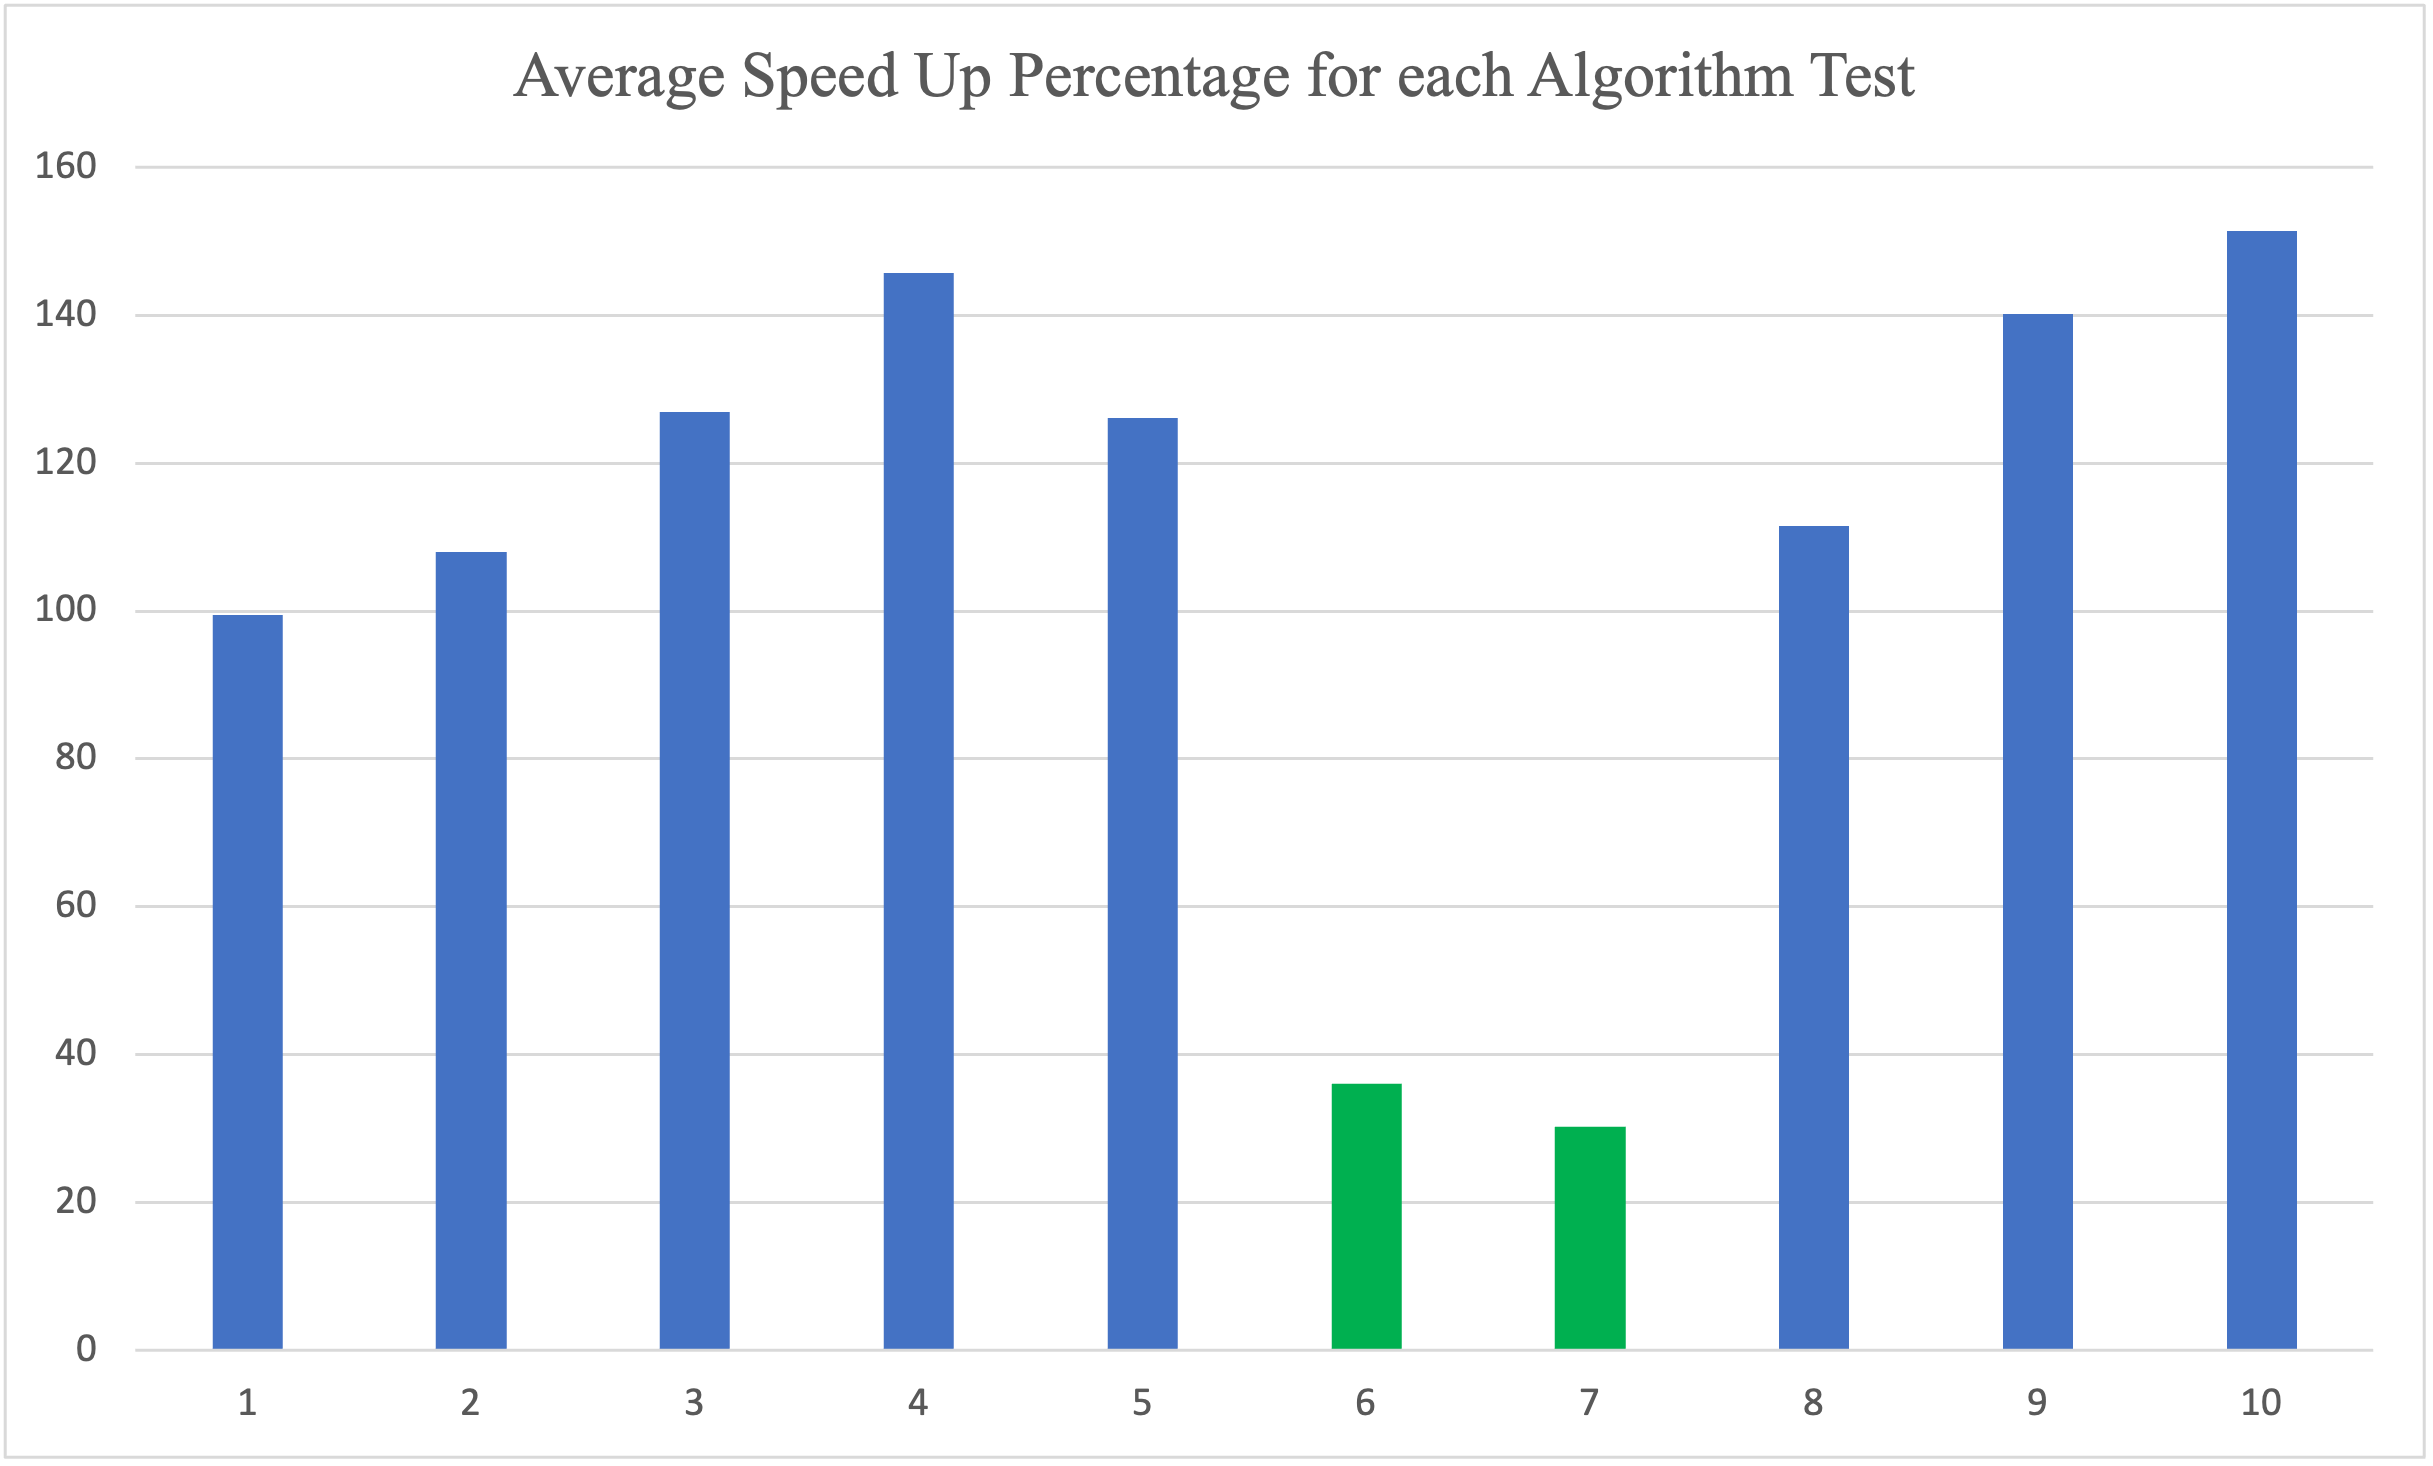
\includegraphics[scale=0.6]{avg-other-per-test}
\caption{\footnotesize{Average performance difference between Flask and Spin on each test, Kruskal is marked green}}
\captionsetup{aboveskip=0pt,font=it}
\end{figure}

\bigskip
\begin{figure}[hp]
\centering
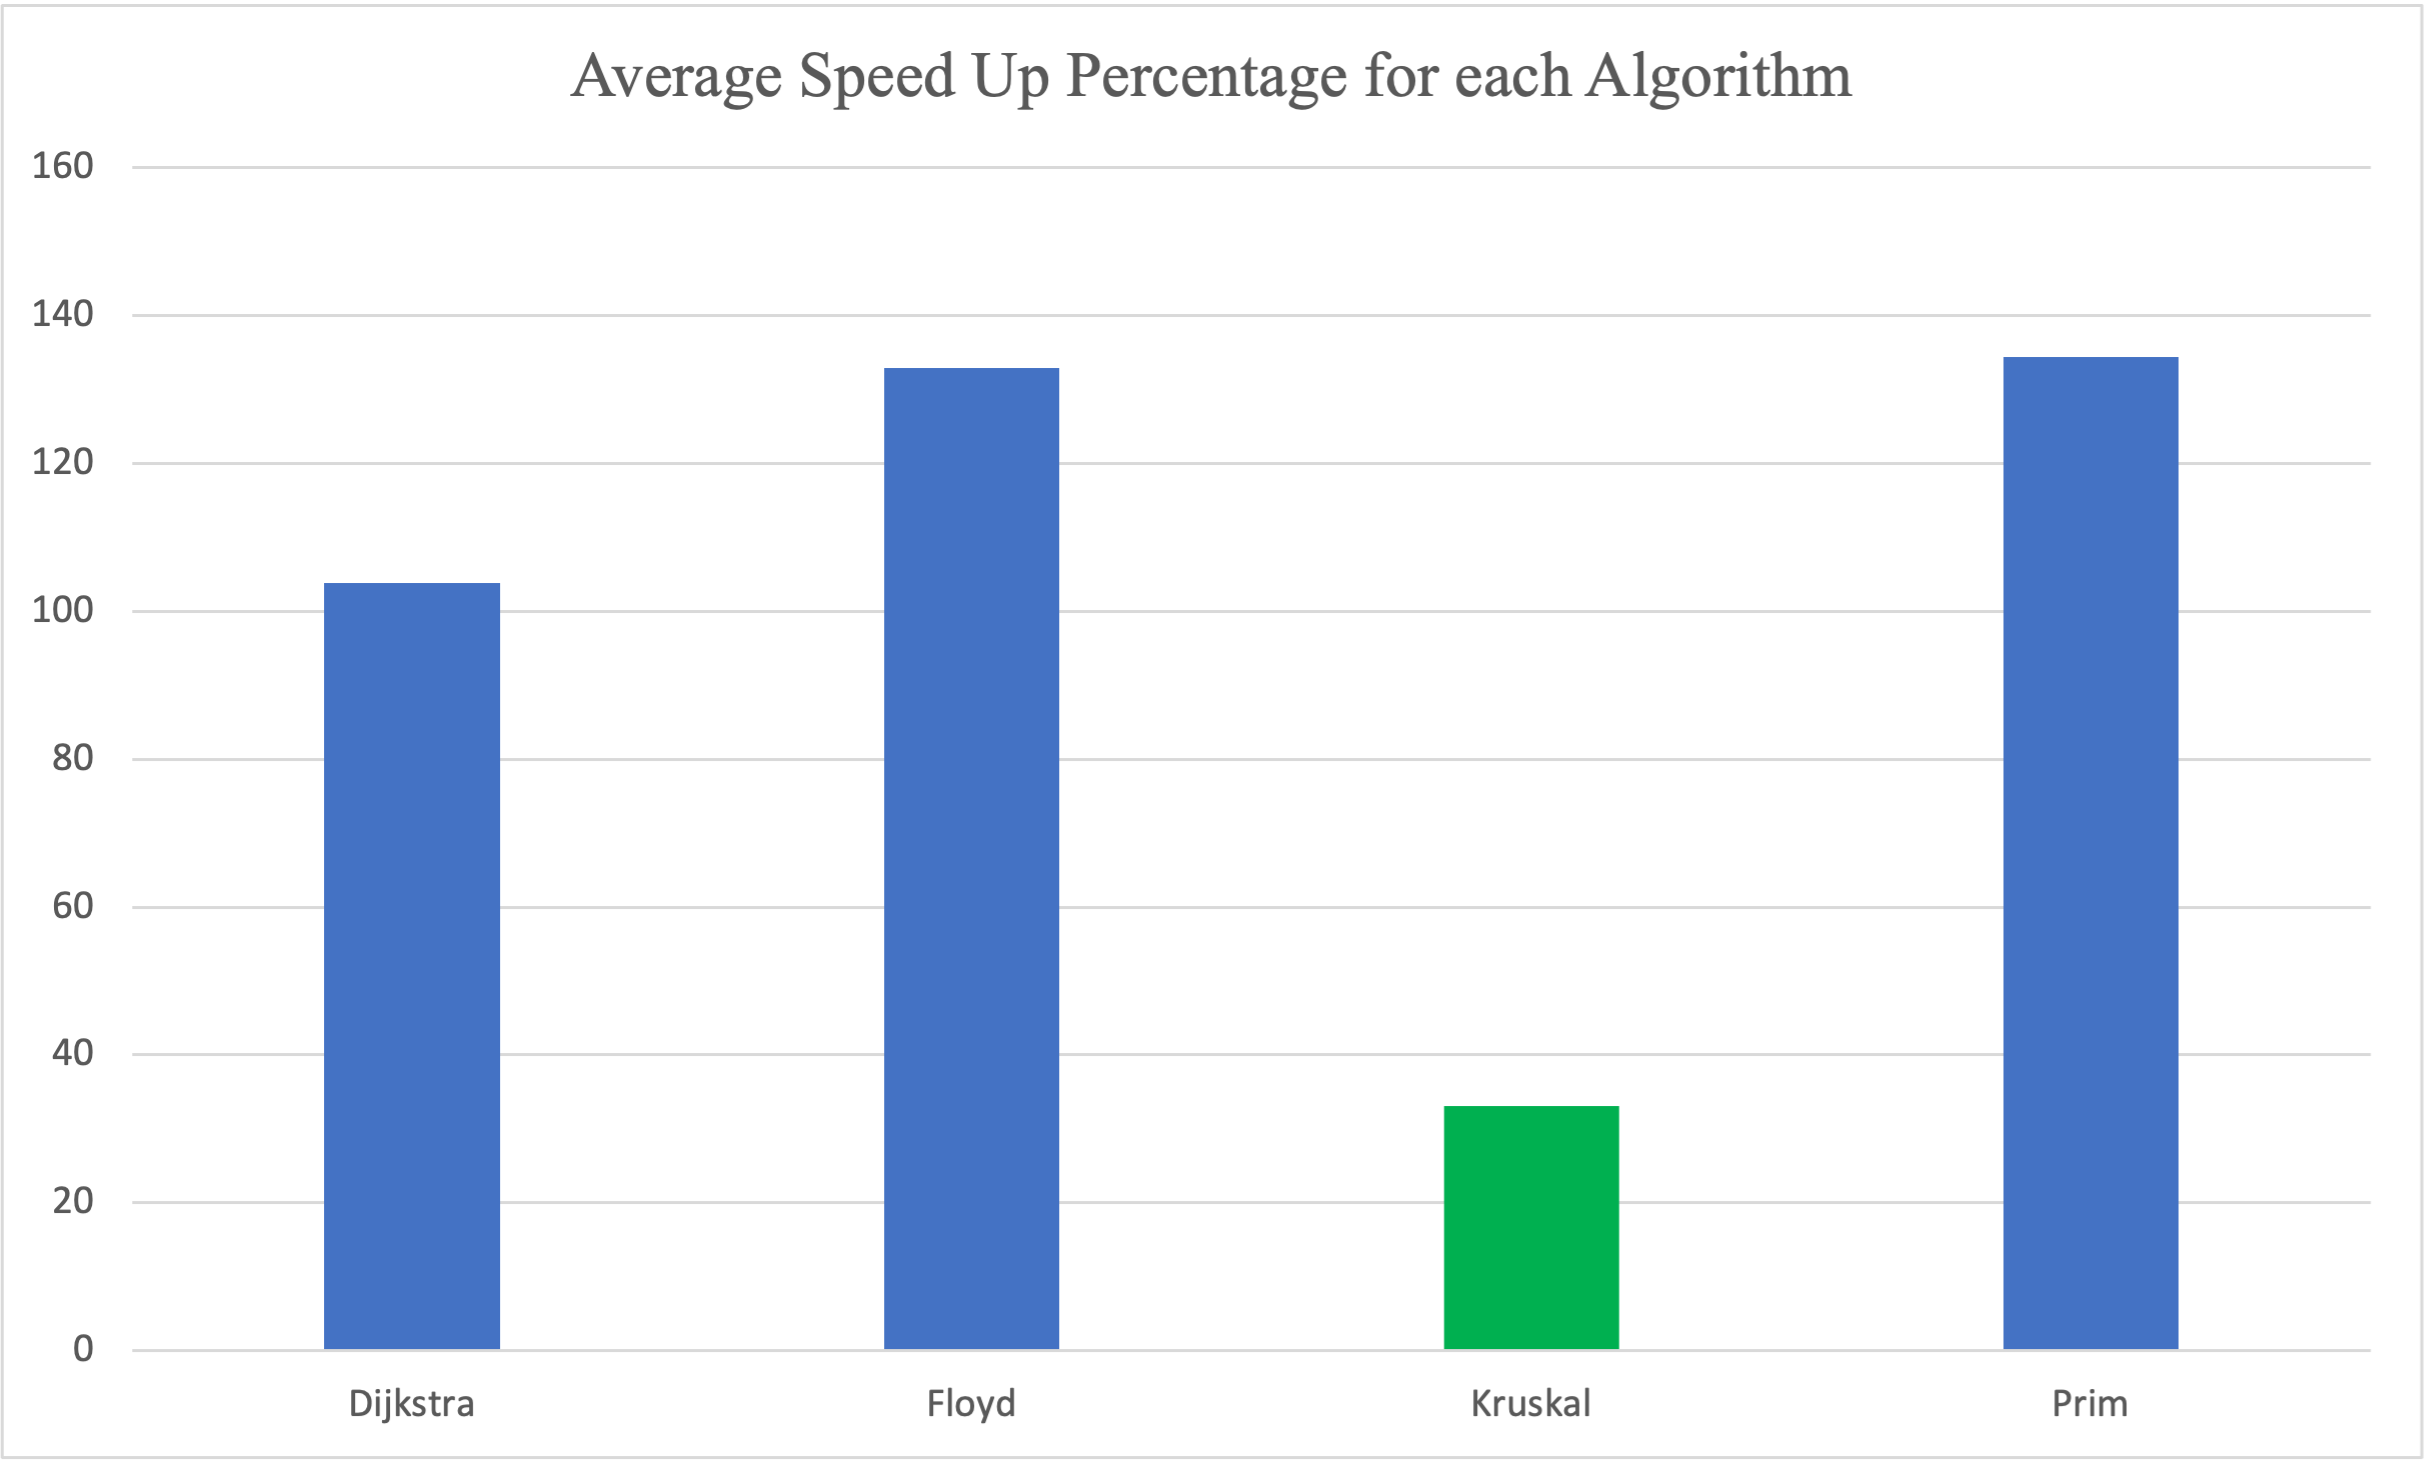
\includegraphics[scale=0.7]{avg-other-per}
\caption{\footnotesize{Average performance difference between Flask and Spin on each benchmarking algorithm, Kruskal is marked green}}
\captionsetup{aboveskip=0pt,font=it}
\end{figure}
\bigskip

We list out the data input size for the shortest path/MST algorithms to explore further. We found that the data input size for Kruskal's algorithm is a lot larger than other 3 other algorithms. The average data input size for Kruskal's algorithm is \textbf{1166666.67}, way larger than the algorithm with the second largest data input size, which is Dijkstra's algorithm with \textbf{4100}. In fact, \textbf{28355.285\%} larger!

\bigskip
\begin{table}[h!]
\centering
\begin{tabular}{||c c c c||} 
\hline
Name & Small & Medium & Large \\ [1ex] 
\hline\hline
 & & & \\
Dijkstra & 2500 & 4000 & 5800 \\ 
 & & & \\
Floyd-Warshall & 180 & 250 & 310 \\ 
 & & & \\
Kruskal & 400000 & 1000000 & 2100000 \\ 
 & & & \\
Prim & 400 & 550 & 680 \\ [1ex]
\hline
\end{tabular}
\caption{Data input sizes for shortest path/MST algorithms}
\label{table:time_complexity_1}
\end{table}
\bigskip

\newpage
\bigskip
\begin{figure}[hp]
\centering
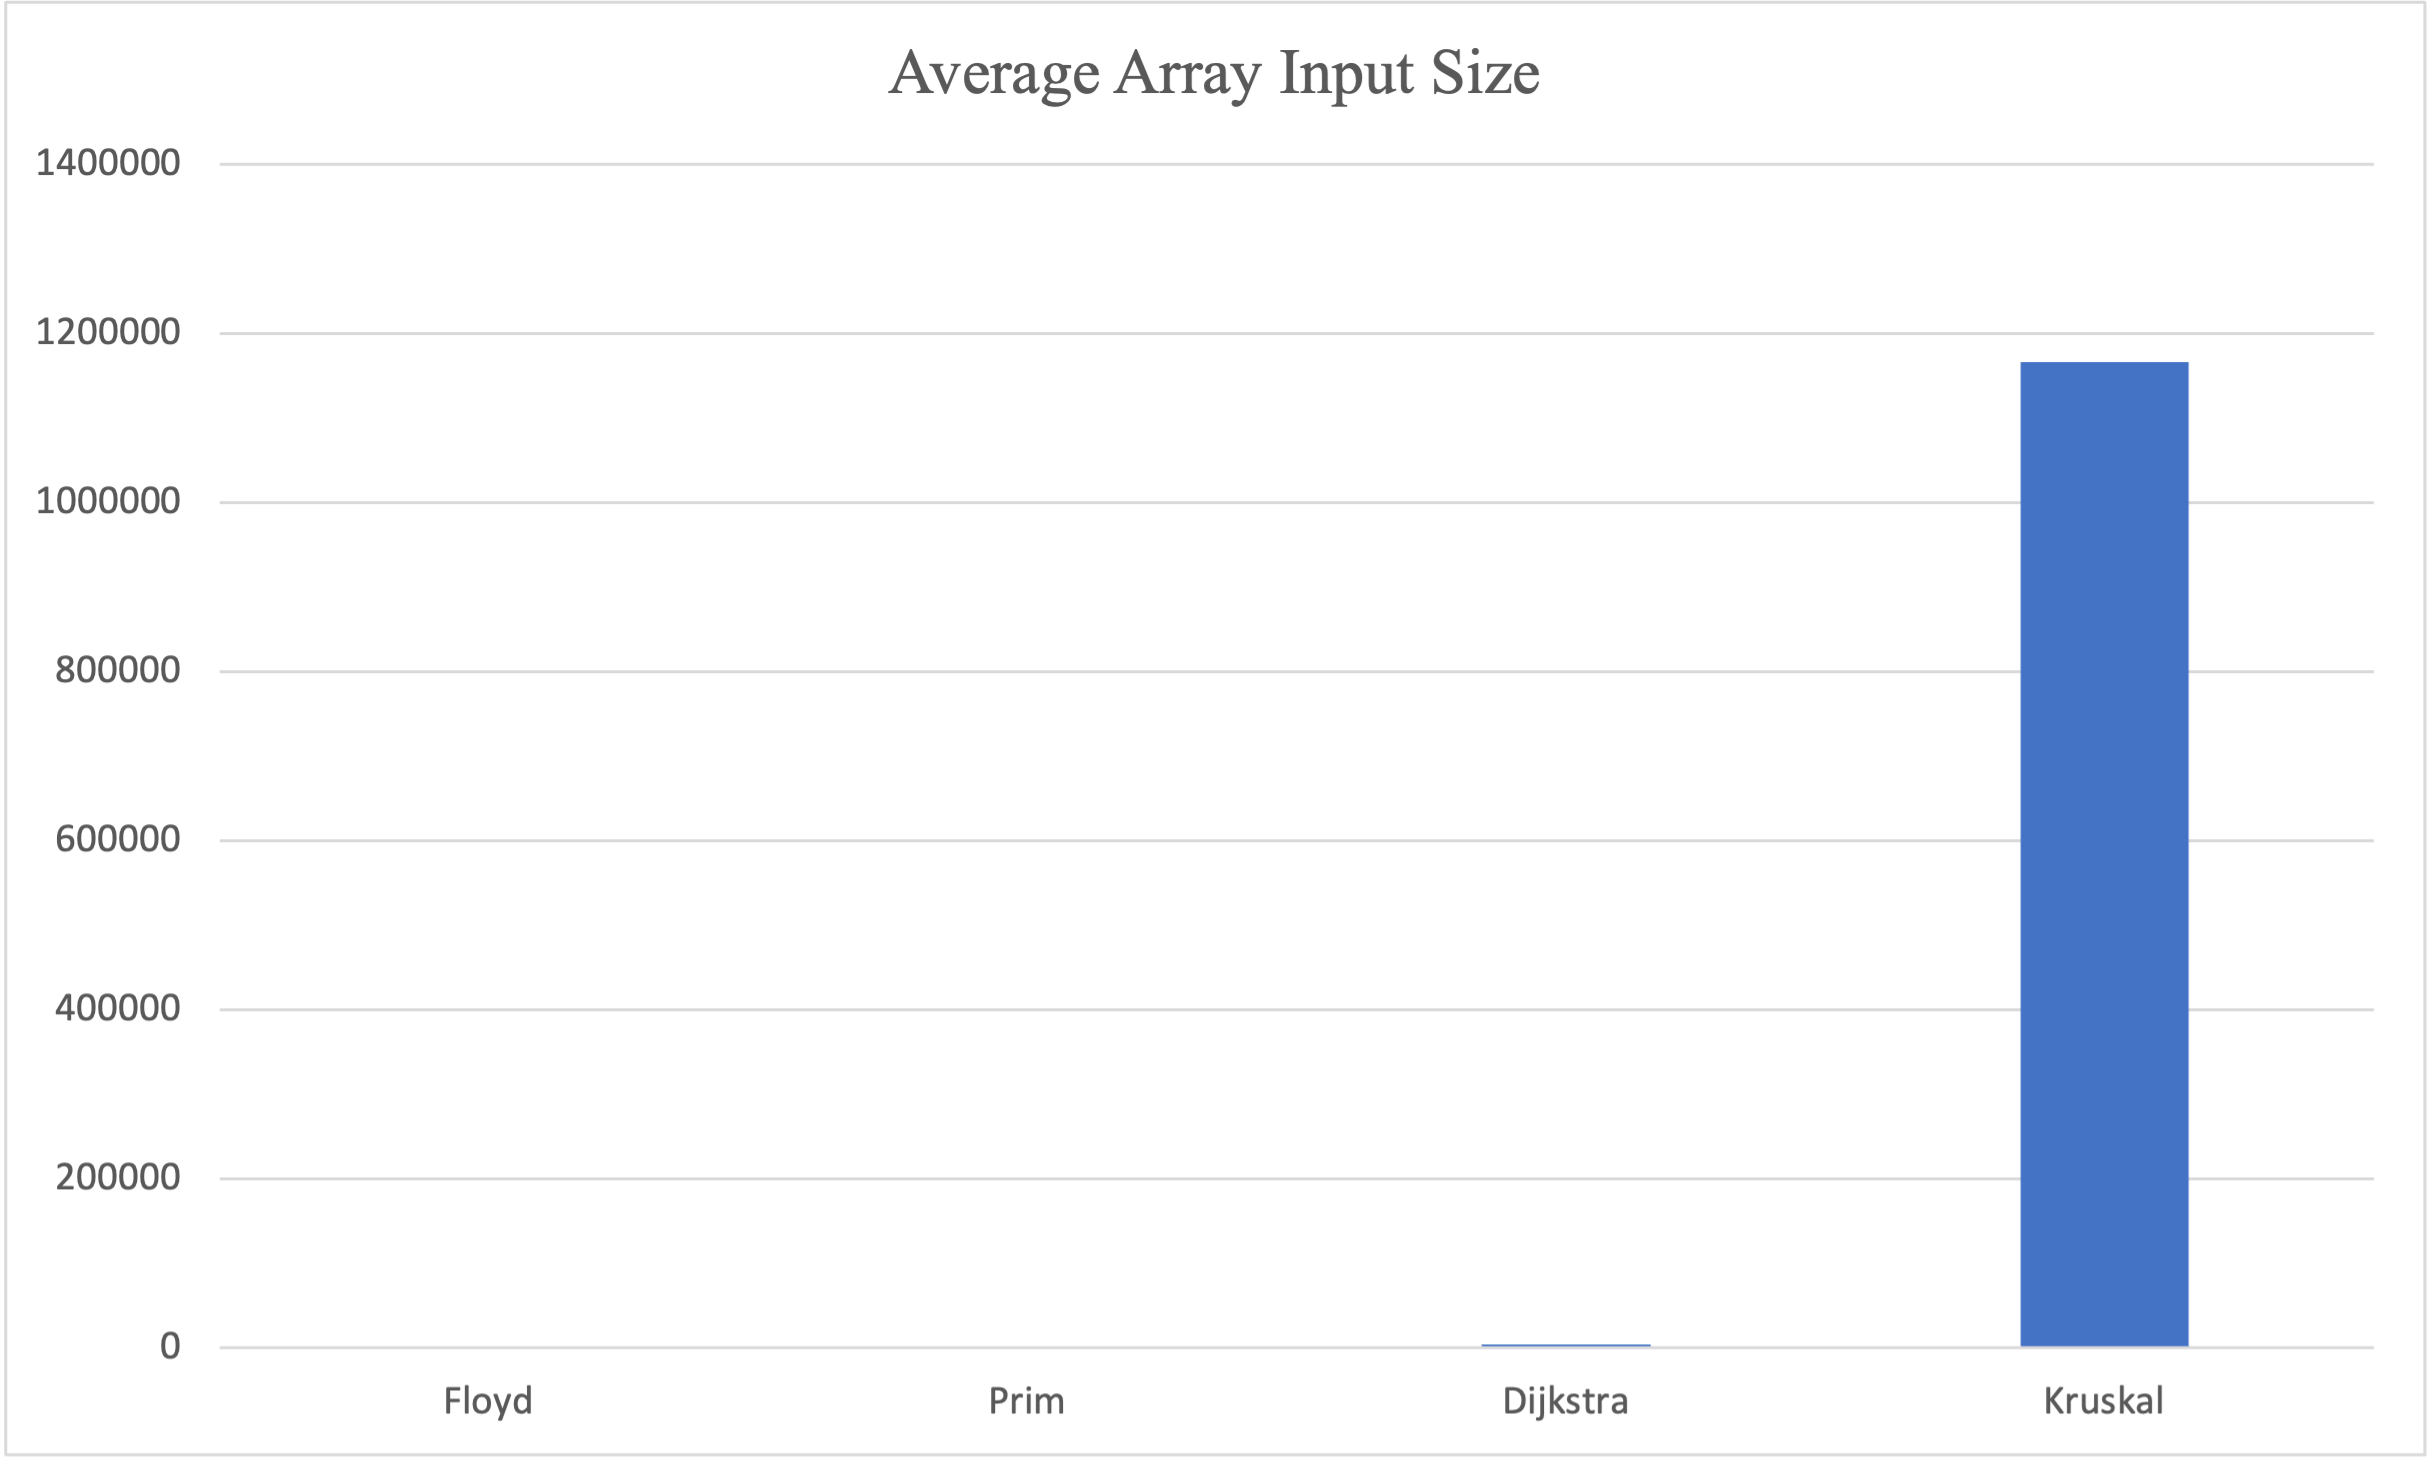
\includegraphics[scale=0.7]{avg-input-size-other}
\caption{\footnotesize{Average data input size for shortest path/MST algorithms (Sorted from small to large). Floyd and Prim's data input sizes are so small in contrast to Kruskal that we cannot see them at all in the graph}}
\captionsetup{aboveskip=0pt,font=it}
\end{figure}
\bigskip

From the table and the chart above, we recognise that there could be a correlation between the data input size with the average algorithm performance difference. This is a solid discovery as it is very much in alignment with the behaviour on the benchmarks for sorting algorithms' performance in the first stage of the experiment. In this case, the algorithm with the lowest performance difference \textbf{(Kruskal's algorithm)} also simultaneously has the largest data input size.

\subsection{Standard Deviation Analysis}

Just like in the first stage of the experiment, we ran each shortest path/MST algorithm \textbf{5} times to ensure the result data we get is consistent.

\bigskip
\begin{table}[h!]
\centering
\begin{tabular}{||c c c c||} 
\hline
Name & Standard Deviation ($\sigma$) & Confidence Interval & 95\% Confidence Interval \\ [1ex] 
\hline\hline
 & & & \\
Dijkstra (S) & 0.04 & 0.018 & 1.5632 ±0.0351 (±2.24\%) \\
 & & & \\
Dijkstra (M) & 0.044 & 0.02 & 4.1416 ±0.0385 (±0.93\%) \\
 & & & \\
Floyd (S) & 0.118 & 0.053 & 1.598 ±0.103 (±6.47\%) \\
 & & & \\
Floyd (M) & 0.109 & 0.049 & 3.8298 ±0.0955 (±2.49\%) \\
 & & & \\
Floyd (L) & 0.757 & 0.339 & 7.9802 ±0.664 (±8.32\%) \\
 & & & \\
Kruskal (S) & 0.167 & 0.075 & 1.853 ±0.146 (±7.88\%) \\
 & & & \\
Kruskal (M) & 0.28 & 0.125 & 4.9848 ±0.246 (±4.93\%) \\
 & & & \\
Prim (S) & 0.143 & 0.064 & 2.0054 ±0.125 (±6.23\%) \\
 & & & \\
Prim (M) & 0.089 & 0.04 & 4.9632 ±0.0782 (±1.58\%) \\
 & & & \\
Prim (L) & 0.147 & 0.066 & 9.3292 ±0.129 (±1.38\%) \\
 & & & \\
Dijkstra (S) & 0.137 & 0.061 & 3.119 ±0.12 (±3.86\%) \\
 & & & \\
Dijkstra (M) & 0.509 & 0.228 & 8.6162 ±0.446 (±5.18\%) \\
 & & & \\
Dijkstra (L) & 0.562 & 0.251 & 18.6322 ±0.492 (±2.64\%) \\
 & & & \\
Floyd (S) & 0.274 & 0.123 & 3.6254 ±0.24 (±6.63\%) \\
 & & & \\
Floyd (M) & 0.327 & 0.146 & 9.4122 ±0.286 (±3.04\%) \\
 & & & \\
Floyd (L) & 0.649 & 0.29 & 18.0462 ±0.569 (±3.15\%) \\
 & & & \\
Kruskal (S) & 0.232 & 0.104 & 2.5208 ±0.203 (±8.05\%) \\ [1ex]
\hline
\end{tabular}
\caption{Standard deviation for Flask framework}
\label{table:time_complexity_2}
\end{table}
\bigskip

\newpage
\bigskip
\begin{table}[h!]
\centering
\begin{tabular}{||c c c c||} 
\hline
Name & Standard Deviation ($\sigma$) & Confidence Interval & 95\% Confidence Interval \\ [1ex] 
\hline\hline
 & & & \\
Kruskal (M) & 0.439 & 0.196 & 6.4914 ±0.385 (±5.93\%) \\
 & & & \\
Kruskal (L) & 0.842 & 0.377 & 15.0142 ±0.738 (±4.92\%) \\
 & & & \\
Prim (S) & 0.22 & 0.098 & 4.2422 ±0.193 (±4.55\%) \\
 & & & \\
Prim (M) & 0.76 & 0.34 & 11.9216 ±0.666 (±5.58\%) \\
 & & & \\
Prim (L) & 1.049 & 0.469 & 23.4506 ±0.919 (±3.92\%) \\ [1ex]
\hline
\end{tabular}
\caption{Standard deviation for Flask framework (continued)}
\label{table:time_complexity_2}
\end{table}
\bigskip

In the above analysis for the standard deviation, similar to the discovery we made during the first stage of the experiment, we discovered that the larger the input data, the larger the standard deviation for the algorithm. For Flask, the average standard deviation for small input data size is \textbf{0.117} while the average standard deviation for large input data size is \textbf{0.452}, a \textbf{286.33\%} increase. This is even more visible when we look at the standard deviation for Spin benchmarks, the average standard deviation for small input data size is \textbf{0.216}, and the average standard deviation for large input data size is \textbf{0.776}. We are able to observe a similar increase in standard deviation at \textbf{286.33\%}.

\bigskip
\begin{figure}[hp]
\centering
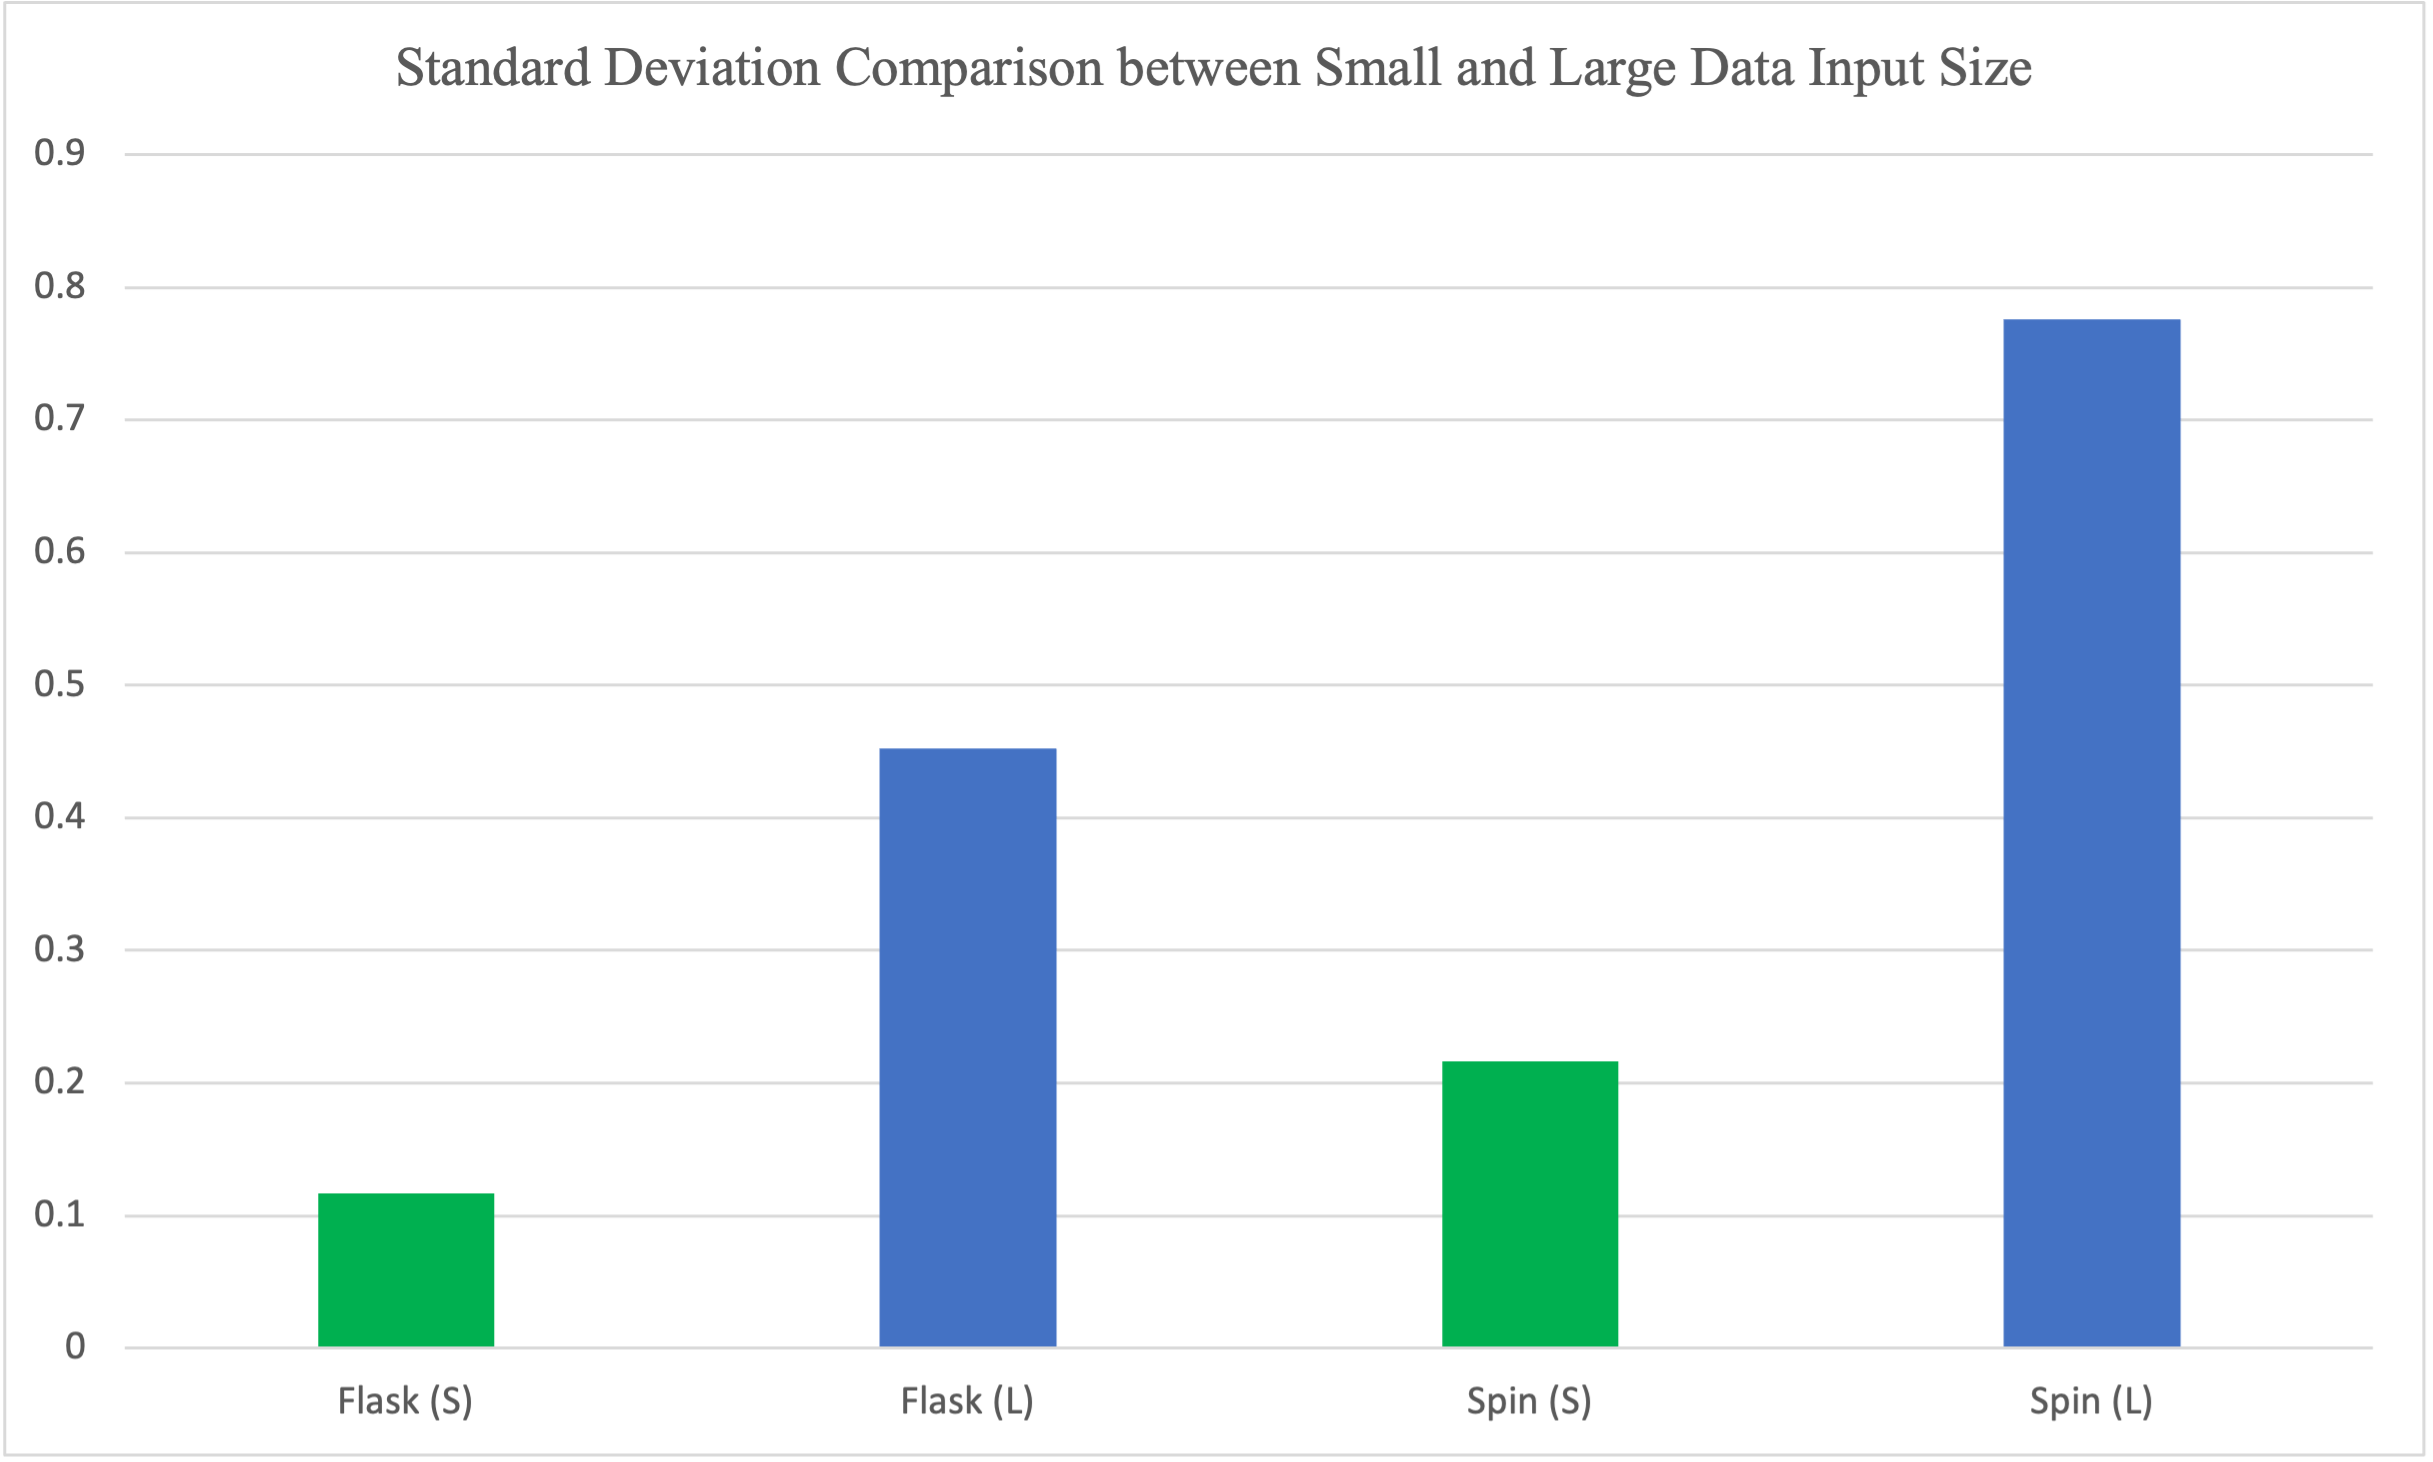
\includegraphics[scale=0.7]{sd-comp}
\caption{\footnotesize{Standard deviation comparison between small and large data input size on both Flask and Spin framework}}
\captionsetup{aboveskip=0pt,font=it}
\end{figure}
\bigskip
\chapter{Discussion} \label{chap:discussion}

After completing the experiment and collecting the result, we would like to review and revisit the procedure, including the experiment setup, execution and analysis of the result data. The experiment largely did not align with the initial hypothesis and assumption: Spin outperforms Flask. Instead, we got the opposite result. Nonetheless, the result was interesting because it made us wonder why Spin did not outperform Flask. Although WebAssembly has shown great potential in its performance throughout its usage in frontend development, we will provide our own verdict on if it is ready to be adopted widely for backend usage, especially within the commercial sector.

We did see areas where WebAssembly performed well. For example, in bucket sorting in the first stage of the experiment, WebAssembly showcased its ability for system memory management. And thus, it outperformed Flask on that particular benchmarking algorithm. We also discovered in the investigation that WebAssembly performed better the larger the input data size, again showcasing that WebAssembly is able to work better with system memory than the traditional implementation. This also aligns with the previous research conducted by Gadepalli et al. (2020) \cite{lit34}.

We list out a few reasons for WebAssembly failed to outperform traditional frameworks. Firstly, the setup. Although \textbf{Amazon Web Service (AWS)} is getting more advanced and powerful every day. It does not have an official way to deploy WebAssembly Applications efficiently. Therefore, we had to use the Amazon EC2 virtual machine service for our experiment for both applications. Furthermore, we used Docker to Containerise our applications. Both procedures add unnecessary overhead to the WebAssembly framework. However, from earlier research and literature reviews, we knew that the main issue with the containerised application is the cold start speed. However, this is a relatively minor concern in our experiment, as our primary goal is to benchmark the calculation ability for both frameworks.

Secondly, we conducted our benchmarking experiment with the Python language. The reason we used Python to conduct the experiment is that Python has the most comprehensive sorting algorithm collections available. In addition, Python is also one of the most popular languages used within the industry. Therefore, it will likely be continuously used across the industry to build new applications with the WebAssembly framework solutions.

Throughout our experiment, from the development of the benchmarking application to local testing, all the way to the deployment of the solution, we constantly noticed that the Spin WebAssembly solution had a worse development experience and a slower runtime than the traditional Flask solution. Thus, WebAssembly has consistently shown its potential within the frontend web development industry and was endorsed by large technology corporations such as \textbf{Adobe} and \textbf{Google}. We believe that it is currently not ready for production development in the backend framework industry, especially within the commercial market. This is also pointed out by the developers of the current WebAssembly backend solutions. For example, Fermyon (Developer for Spin framework) and the Wasmcloud team. However, considering the technology was first made available in 2019 with the release of \textbf{WASI (WebAssembly System Interface)}, it has made considerable progress in only a few years. Thus, continuing with the current development rate, we can see the huge potential of the WebAssembly backend solution running on the edge.

Continuing from what we uncovered during the experiment, we propose a few possible areas for further research. Firstly, we discovered that the performance gap between the WebAssembly solution and the traditional Flask solution decreases when the input data size increases. Thus, we propose to expand our existing experiment, potentially adding support to our current benchmarking applications to accept larger input data. After that, re-run the experiment procedure.

Secondly, we propose to re-implement our experiment with a high-performance programming language, such as \textbf{Go} or \textbf{Rust}, at the same time keeping the current deployment procedure. Recently, languages such as Rust have gained considerable popularity along with the rise of WebAssembly. Although Python continues to remain one of the most popular programming languages, developers and researchers have gradually switched to the Go and Rust programming language for server-side WebAssembly solution development. Thus, it is worth re-conducting our experiment with a high-performing language to further solidify our current discoveries from the experiments in this thesis.
\chapter{Conclusion} \label{chap:conclusion}

The conclusion goes here.




%%%%%%%%%%%%
% End

% Bibliography
% \bibliographystyle{style/mybibstyle}
% {
%     \setstretch{1.25}
%     \cleardoublepage
%     \phantomsection
%     \bibliography{references}
% }

\begin{thebibliography}{9}
\bibitem{abs1}
"What is Colossus?," www.computerhope.com. https://www.computerhope.com/jargon/c/colossus.htm

\bibitem{abs2}
Wikipedia Contributors, "Dot-com bubble," Wikipedia, Mar. 21, 2019. https://en.wikipedia.org/wiki/Dot-com\_bubble

\bibitem{abs3}
Booking.com, "Booking.com: The largest selection of hotels, homes, and vacation rentals," Booking.com, 2019. https://www.booking.com/

\bibitem{abs4}
eBay, "Electronics, Cars, Fashion, Collectibles, Coupons and More | eBay," eBay, 2019. https://www.ebay.com/

\bibitem{abs5}
Figma, "Figma: the collaborative interface design tool.," Figma, 2019. https://www.figma.com/

\bibitem{abs6}
"Roadmap - WebAssembly," webassembly.org. https://webassembly.org/roadmap/

\bibitem{abs7}
"Made with WebAssembly," madewithwebassembly.com. https://madewithwebassembly.com/

\bibitem{abs8}
"Figma is powered by WebAssembly," Figma, Jun. 08, 2017. https://www.figma.com/blog/webassembly-cut-figmas-load-time-by-3x/

\bibitem{abs9}
J. Kastrenakes, "Adobe brings a simplified Photoshop to the web," The Verge, Oct. 26, 2021. https://www.theverge.com/2021/10/26/22738125/adobe-photoshop-illustrator-web-announced (accessed Nov. 05, 2022).

\bibitem{abs10}
P. Clark, "Photoshop ships major updates across desktop and iPad apps; Extends Light Editing and Collaboration features to the web (beta)|Adobe," Adobe Blog. https://blog.adobe.com/en/publish/2021/10/26/photoshop-ships-major-updates-across-desktop-ipad-apps-extends-light-editing-collaboration-features-web-beta (accessed Nov. 05, 2022).

\bibitem{abs11}
"Photoshop’s journey to the web," web.dev. https://web.dev/ps-on-the-web/ (accessed Nov. 05, 2022).

\bibitem{abs12}
B. Spies and M. Mock, "An Evaluation of WebAssembly in Non-Web Environments," 2021 XLVII Latin American Computing Conference (CLEI), 2021, pp. 1-10, doi: 10.1109/CLEI53233.2021.9640153.

\bibitem{abs13}
A. Jangda, B. Powers, E. Berger, and A. Guha, “Not so fast: Analyzing the performance of WebAssembly vs. Native code,” arXiv [cs.PL], 2019.

\bibitem{int1}
"WWDC 2017 — APPOCALYPSE — Apple," www.youtube.com. https://www.youtube.com/watch?v=mPnl1aazs98

\bibitem{int2}
Google, "Google Scholar," Google.com.au, 2019. https://scholar.google.com.au/

\bibitem{int3}
"The New England Journal of Medicine: Research \& Review Articles on Disease \& Clinical Practice," New England Journal of Medicine, 2000. https://www.nejm.org/

\bibitem{int4}
J. Bergdahl, "JS is weird," jacobbergdahl.com. https://jsisweird.com/ (accessed Nov. 05, 2022).

\bibitem{int5}
"Documentation - TypeScript for the New Programmer," www.typescriptlang.org. https://www.typescriptlang.org/docs/handbook/typescript-from-scratch.html

\bibitem{int6}
"Why You Should Use React.js For Web Development," freeCodeCamp.org, Feb. 18, 2021. https://www.freecodecamp.org/news/why-use-react-for-web-development (accessed Nov. 05, 2022).

\bibitem{int7}
"Inventing the Internet," www.youtube.com. https://www.youtube.com/watch?v=BnFJ8cHAlco (accessed Nov. 05, 2022).

\bibitem{int8}
A. Gore, "S.272 - 102nd Congress (1991-1992): High-Performance Computing Act of 1991," www.congress.gov, Dec. 09, 1991. https://www.congress.gov/bill/102nd-congress/senate-bill/272

\bibitem{int9}
"NCSA Mosaic -- September 10, 1993 Demo," totic.org. http://totic.org/nscp/demodoc/demo.html (accessed Nov. 05, 2022).

\bibitem{int10}
T. B. Lee, "The internet, explained," Vox, Jun. 16, 2014. https://www.vox.com/2014/6/16/18076282/the-internet

\bibitem{int11}
"A Brief History of JavaScript," DEV Community. https://dev.to/dboatengx/history-of-javascript-how-it-all-began-92a

\bibitem{int12}
Oracle.com, 2022. https://developer.oracle.com/javascript/what-is-javascript/ (accessed Nov. 05, 2022).

\bibitem{int13}
"Microsoft Launches Microsoft Internet Explorer 3.0 With Exclusive, Free Content Offers From Top Web Sites," Stories, Aug. 13, 1996. https://news.microsoft.com/1996/08/13/microsoft-launches-microsoft-internet-explorer-3-0-with-exclusive-free-content-offers-from-top-web-sites/

\bibitem{int14}
"Goodbye, Flash: The web application everybody used — and hated," NBC News, Dec. 31, 2020. Accessed: Jan. 02, 2021. [Online]. Available: https://www.nbcnews.com/tech/internet/goodbye-flash-web-application-everybody-used-hated-n1252607

\bibitem{int15}
"Infographic: The End of the Flash Era," Statista Infographics. https://www.statista.com/chart/3796/websites-using-flash/

\bibitem{int16}
"Adobe Flash Player Enterprise End of Life," www.adobe.com. https://www.adobe.com/products/flashplayer/enterprise-end-of-life.html

\bibitem{inta1}
https://devhumor.com/media/javascript-is-weird

\bibitem{int17}
"WebAssembly," webassembly.org. https://webassembly.org/

\bibitem{int18}
A. Haas et al., "Bringing the web up to speed with WebAssembly", ACM SIGPLAN Notices, vol. 52, no. 6, pp. 185-200, 2017. Available: 10.1145/3140587.3062363.

\bibitem{int19}
A. Jangda, B. Powers, E. Berger, and A. Guha, “Not so fast: Analyzing the performance of WebAssembly vs. Native code,” arXiv [cs.PL], 2019.

\bibitem{int20}
"Polyglot (computing)," Wikipedia, Sep. 23, 2022. https://en.wikipedia.org/wiki/Polyglot\_(computing) (accessed Nov. 05, 2022).

\bibitem{int21}
".NET | Free. Cross-platform. Open Source.," Microsoft. https://dotnet.microsoft.com/en-us/

\bibitem{int22}
Wikipedia Contributors, ".NET Framework," Wikipedia, Apr. 29, 2019. https://en.wikipedia.org/wiki/.NET\_Framework

\bibitem{int23}
Wikipedia Contributors, "Visual Basic .NET," Wikipedia, Apr. 14, 2019. https://en.wikipedia.org/wiki/Visual\_Basic\_.NET

\bibitem{int24}
BillWagner, "C\# docs - get started, tutorials, reference.," learn.microsoft.com. https://learn.microsoft.com/en-us/dotnet/csharp/

\bibitem{int25}
"How to mix C\# and VB.net in the same project," www.cryer.co.uk. https://www.cryer.co.uk/brian/mswinswdev/ms\_dotnet\_mix\_csharp\_and\_vb.htm (accessed Nov. 05, 2022).

\bibitem{int26}
M. Georgescu and D. Milodin, "Open Source Tools to Assist in the Development of Software Applications, " Open Source Science Journal, 2010, Vol. 2, No. 2.

\bibitem{int27}
Node.js Foundation, "Node.js," Node.js, 2019. https://nodejs.org/en/

\bibitem{int28}
Slack, "Where Work Happens," Slack, 2018. https://slack.com/

\bibitem{int29}
Zoom, "Video conferencing, web conferencing, webinars, screen sharing," Zoom Video, 2022. https://zoom.us/

\bibitem{int30}
WhatsApp, "WhatsApp," WhatsApp.com, 2018. https://www.whatsapp.com/

\bibitem{int31}
"V8 JavaScript engine," v8.dev. https://v8.dev/

\bibitem{int32}
adegeo, "Windows Presentation Foundation for .NET 5 documentation," learn.microsoft.com. https://learn.microsoft.com/en-us/dotnet/desktop/wpf/?view=netdesktop-6.0

\bibitem{int33}
QuinnRadich, "UWP Documentation - UWP app developer," learn.microsoft.com. https://learn.microsoft.com/en-us/windows/uwp/ (accessed Nov. 06, 2022).

\bibitem{int34}
"Swing (Java)," Wikipedia, Nov. 17, 2019. https://en.wikipedia.org/wiki/Swing\_(Java)

\bibitem{int35}
deepu, "Visualizing memory management in V8 Engine (JavaScript, NodeJS, Deno, WebAssembly)," Technorage, Jan. 27, 2020. https://deepu.tech/memory-management-in-v8/ (accessed Nov. 06, 2022).

\bibitem{int36}
T. Warren, "Chrome now uses more RAM because of Spectre security fixes," The Verge, Jul. 12, 2018. https://www.theverge.com/2018/7/12/17564064/google-chrome-ram-usage-memory-increase-spectre-fixes (accessed Nov. 06, 2022).

\bibitem{int37}
"Safari," Apple, 2018. https://www.apple.com/safari/

\bibitem{int38}
"macOS Big Sur - Apple," web.archive.org, Oct. 18, 2021. https://web.archive.org/web/20211018064504/https://www.apple.com/macos/big-sur/ (accessed Nov. 06, 2022).

\bibitem{int39}
"Chrome Used 10X More RAM Than Safari on macOS Big Sur in Recent Test [Updated]," MacRumors. https://www.macrumors.com/2021/02/20/chrome-safari-ram-test/ (accessed Nov. 06, 2022).

\bibitem{int40}
"Exploring lighter alternatives to Electron for hosting a Blazor desktop app," Steve Sanderson’s Blog. https://blog.stevensanderson.com/2019/11/01/exploring-lighter-alternatives-to-electron-for-hosting-a-blazor-desktop-app/ (accessed Nov. 06, 2022).

\bibitem{lit1}
"Three Protocols, the | Encyclopedia.com", Encyclopedia.com, 2022. [Online]. Available: https://www.encyclopedia.com/economics/encyclopedias-almanacs-transcripts-and-maps/three- protocols. [Accessed: 02-May-2022].

\bibitem{lit2}
"Roadmap - WebAssembly", Webassembly.org, 2022. [Online]. Available: https://webassembly.org/roadmap/. [Accessed: 02-May-2022].

\bibitem{lit3}
Möller, Andreas \& Michahelles, Florian \& Diewald, Stefan \& Roalter, Luis \& Kranz, Matthias. (2012). Update Behavior in App Markets and Security Implications: A Case Study in Google Play.

\bibitem{lit4}
"App Store," Apple. https://www.apple.com/app-store/

\bibitem{lit5}
"Google Play," Google.com, 2009. https://play.google.com/

\bibitem{lit6}
"Turning Off Auto Updates in Google Chrome", Chromium.org, 2022. [Online]. Available: https://www.chromium.org/administrators/turning-off-auto-updates/. [Accessed: 02-May-2022].

\bibitem{lit7}
Apple Support. 2022. How to manually update apps on your Apple device. [online] Available at: <https://support.apple.com/HT202180> [Accessed 2 May 2022].

\bibitem{lit8}
D. Geer, "Auto-Update Considered Harmful" in IEEE Security \& Privacy, vol. 19, no. 02, pp. 79- 80, 2021. doi: 10.1109/MSEC.2021.3050248

\bibitem{lit9}
B. M. Luettmann and A. C. Bender, "Man-in-the-middle attacks on auto-updating software," in Bell Labs Technical Journal, vol. 12, no. 3, pp. 131-138, Fall 2007, doi: 10.1002/bltj.20255.

\bibitem{lit10}
Insane, Facebook.com. Apr. 2022. [online] Available at: <https://www.facebook.com/TheInsaneApp/posts/532542348235323> [Accessed 2 May 2022].

\bibitem{lit11}
Haas, A., Rossberg, A., Schuff, D., Titzer, B., Holman, M., Gohman, D., Wagner, L., Zakai, A. and Bastien, J., 2017. Bringing the web up to speed with WebAssembly. ACM SIGPLAN Notices, 52(6), pp.185-200.

\bibitem{lit12}
"Benchmark of WebAssembly runtimes - 2021 Q1 | Frank DENIS random thoughts.," 00f.net. https://00f.net/2021/02/22/webassembly-runtimes-benchmarks/ (accessed Oct. 02, 2022).

\bibitem{lit13}
Microsoft. 2022. Blazor | Build client web apps with C\# | .NET. [online] Available at: <https://dotnet.microsoft.com/en-us/apps/aspnet/web-apps/blazor> [Accessed 2 May 2022].

\bibitem{lit14}
Micha Reiser and Luc Bläser. 2017. Accelerate JavaScript applications by cross-compiling to WebAssembly. In Proceedings of the 9th ACM SIGPLAN International Workshop on Virtual Machines and Intermediate Languages (VMIL 2017). Association for Computing Machinery, New York, NY, USA, 10–17. https://doi.org/10.1145/3141871.3141873

\bibitem{lit15}
David Herman, Wagner Luke, and Alon Zakai. 2014. asm.js. (2014). https://goo.gl/sxWVss

\bibitem{lit16}
Yutian Yan, Tengfei Tu, Lijian Zhao, Yuchen Zhou, and Weihang Wang. 2021. Understanding the performance of webassembly applications. In Proceedings of the 21st ACM Internet Measurement Conference (IMC '21). Association for Computing Machinery, New York, NY, USA, 533–549. https://doi.org/10.1145/3487552.3487827

\bibitem{lit17}
BenchmarkingWebAssembly. 2022. Input Size. [online] Available at: <https://benchmarkingwasm.github.io/BenchmarkingWebAssembly/input\_size.html> [Accessed 2 May 2022].

\bibitem{lit18}
W3schools.com. 2022. JavaScript History. [online] Available at: <https://www.w3schools.com/js/js\_history.asp> [Accessed 2 May 2022].

\bibitem{lit19}
"History of WebAssembly (Chrome University 2019)," www.youtube.com. https://www.youtube.com/watch?v=6r0NKEQqkz0 (accessed Oct. 02, 2022).

\bibitem{lit20}
Jangda, A., Powers, B., Berger, E. D., \& Guha, A. (2019). Not So Fast: Analyzing the Performance of WebAssembly vs. Native Code. 2019 USENIX Annual Technical Conference (USENIX ATC 19), 107–120. https://www.usenix.org/conference/atc19/presentation/jangda

\bibitem{lit21}
Browsix.org. 2022. Browsix: Unix in the browser tab. [online] Available at: <https://browsix.org/> [Accessed 2 May 2022].

\bibitem{lit22}
Node.js. 2022. Node.js. [online] Available at: <https://nodejs.org/> [Accessed 2 May 2022].

\bibitem{lit23}
GitHub. 2022. GitHub - gwsystems/aWsm: WebAssembly ahead-of-time compiler and runtime. Focuses on generating fast code, simplicity, and portability.. [online] Available at: <https://github.com/gwsystems/aWsm> [Accessed 2 May 2022].

\bibitem{lit24}
Wasmer.io. 2022. Wasmer - The Universal WebAssembly Runtime. [online] Available at: <https://wasmer.io/> [Accessed 2 May 2022].

\bibitem{lit25}
E. Wen and G. Weber, "Wasmachine: Bring IoT up to Speed with A WebAssembly OS," 2020 IEEE International Conference on Pervasive Computing and Communications Workshops (PerCom Workshops), 2020, pp. 1-4, doi: 10.1109/PerComWorkshops48775.2020.9156135.

\bibitem{lit26}
E. Wen and G. Weber, "Wasmachine: Bring the Edge up to Speed with A WebAssembly OS," 2020 IEEE 13th International Conference on Cloud Computing (CLOUD), 2020, pp. 353-360, doi: 10.1109/CLOUD49709.2020.00056.

\bibitem{lit27}
F. Eriksson and S. Grunditz, ‘Containerizing WebAssembly : Considering WebAssembly Containers on IoT Devices as Edge Solution’, Dissertation, 2021.

\bibitem{lit28}
Docker, "Enterprise Application Container Platform | Docker," Docker, 2018. https://www.docker.com/

\bibitem{lit29}
J. Napieralla, “Considering WebAssembly Containers for Edge Computing on Hardware-Constrained IoT Devices”, 2020.

\bibitem{lit30}
Amazon Web Services, Inc. 2022. Serverless Computing - AWS Lambda - Amazon Web Services. [online] Available at: <https://aws.amazon.com/lambda/> [Accessed 2 May 2022].

\bibitem{lit31}
Eismann, S., Scheuner, J., van Eyk, E., Schwinger, M., Grohmann, J., Herbst, N., Abad, C. L., \& Iosup, A. (2021). Serverless Applications: Why, When, and How? IEEE Software, 38(1), 32–39. https://doi.org/10.1109/ms.2020.3023302

\bibitem{lit32}
Gackstatter, P. (2021). A WebAssembly Container Runtime for Serverless Edge Computing (Doctoral dissertation, Wien). https://doi.org/10.34726/hss.2021.85181

\bibitem{lit33}
P. K. Gadepalli, G. Peach, L. Cherkasova, R. Aitken and G. Parmer, "Challenges and Opportunities for Efficient Serverless Computing at the Edge," 2019 38th Symposium on Reliable Distributed Systems (SRDS), 2019, pp. 261-2615, doi: 10.1109/SRDS47363.2019.00036.

\bibitem{lit34}
Phani Kishore Gadepalli, Sean McBride, Gregor Peach, Ludmila Cherkasova, and Gabriel Parmer. 2020. Sledge: a Serverless-first, Light-weight Wasm Runtime for the Edge. In Proceedings of the 21st International Middleware Conference (Middleware '20). Association for Computing Machinery, New York, NY, USA, 265–279. https://doi.org/10.1145/3423211.3425680

\bibitem{lit35}
"Nuclio", nuclio, 2022. [Online]. Available: https://nuclio.io/. [Accessed: 02- May- 2022].

\bibitem{lit36}
Kubernetes, "Production-Grade Container Orchestration," Kubernetes.io, 2019. https://kubernetes.io/

\bibitem{lit37}
M. Nieke, L. Almstedt, and R. Kapitza, "Edgedancer," Proceedings of the 4th International Workshop on Edge Systems, Analytics and Networking, Apr. 2021, doi: 10.1145/3434770.3459731.

\bibitem{lit38}
I. Pelle, J. Czentye, J. Dóka, A. Kern, B. P. Gerő and B. Sonkoly, "Operating Latency Sensitive Applications on Public Serverless Edge Cloud Platforms," in IEEE Internet of Things Journal, vol. 8, no. 10, pp. 7954-7972, 15 May15, 2021, doi: 10.1109/JIOT.2020.3042428.

\bibitem{lit39}
OpenCV, "OpenCV library," Opencv.org, 2019. https://opencv.org/

\bibitem{lit40}
"AWS IoT Greengrass - Amazon Web Services," Amazon Web Services, Inc., 2019. https://aws.amazon.com/greengrass/

\bibitem{lit41}
M. Xu et al., "From cloud to edge: a first look at public edge platforms," Proceedings of the 21st ACM Internet Measurement Conference, Nov. 2021, doi: 10.1145/3487552.3487815.

\bibitem{lit42}
"Extending the Boundaries of the Cloud with Edge Computing," Alibaba Cloud Community. https://www.alibabacloud.com/blog/extending-the-boundaries-of-the-cloud-with-edge-computing\_594214 (accessed Oct. 02, 2022).

\bibitem{lit43}
P. Gackstatter, P. A. Frangoudis and S. Dustdar, "Pushing Serverless to the Edge with WebAssembly Runtimes," 2022 22nd IEEE International Symposium on Cluster, Cloud and Internet Computing (CCGrid), 2022, pp. 140-149, doi: 10.1109/CCGrid54584.2022.00023.

\bibitem{lit44}
"Cloud Functions," Google Cloud. https://cloud.google.com/functions

\bibitem{lit45}
Apache OpenWhisk is a serverless, open source cloud platform," openwhisk.apache.org. https://openwhisk.apache.org/

\bibitem{eva1}
Amazon, "Amazon Web Services (AWS) - Cloud Computing Services," Amazon Web Services, Inc., 2022. https://aws.amazon.com/

\bibitem{eva2}
Google, "Cloud Computing Services  |  Google Cloud," Google Cloud, 2019. https://cloud.google.com/

\bibitem{eva3}
"Cloud Computing Services | Microsoft Azure," azure.microsoft.com. https://azure.microsoft.com

\bibitem{eva4}
"The Best Python Web Frameworks 2022," DEV Community. https://dev.to/theme\_selection/the-best-python-web-frameworks-d2d

\bibitem{exp1}
"Google Trends," Google Trends. https://trends.google.com/trends/explore?date=today\%205-y\&q=Edge\%20Computing (accessed Nov. 06, 2022).

\bibitem{exp2}
"Cloud Functions for Firebase," Firebase. https://firebase.google.com/docs/functions

\bibitem{exp3}
Cloudflare, "Cloudflare Workers, " Cloudflare.com, 2019. https://workers.cloudflare.com/ (accessed Dec. 30, 2019).

\bibitem{exp4}
"Next.js by Vercel - The React Framework," nextjs.org. https://nextjs.org/

\bibitem{exp5}
"Edge Network," Vercel Documentation. https://vercel.com/docs/concepts/edge-network/overview (accessed Nov. 06, 2022).

\bibitem{exp6}
Phani Kishore Gadepalli, Sean McBride, Gregor Peach, Ludmila Cherkasova, and Gabriel Parmer. 2020. Sledge: a Serverless-first, Light-weight Wasm Runtime for the Edge. In Proceedings of the 21st International Middleware Conference (Middleware '20). Association for Computing Machinery, New York, NY, USA, 265–279. https://doi.org/10.1145/3423211.3425680

\bibitem{exp7}
AWS, "AWS Lambda – Serverless Compute - Amazon Web Services," Amazon Web Services, Inc., 2019. https://aws.amazon.com/lambda/

\bibitem{exp8}
ggailey777, "Azure Functions documentation," docs.microsoft.com. https://docs.microsoft.com/en-us/azure/azure-functions/

\bibitem{exp9}
"Cloud Functions," Google Cloud. https://cloud.google.com/functions

\bibitem{exp10}
"Apache OpenWhisk is a serverless, open source cloud platform," openwhisk.apache.org. https://openwhisk.apache.org/

\bibitem{exp11}
Wikipedia Contributors, "Web framework," Wikipedia, Apr. 03, 2020. https://en.wikipedia.org/wiki/Web\_framework

\bibitem{exp12}
Wikipedia Contributors, "Web application," Wikipedia, Aug. 16, 2019. https://en.wikipedia.org/wiki/Web\_application

\bibitem{exp13}
Facebook, "React – A JavaScript library for building user interfaces," Reactjs.org, 2022. https://reactjs.org/

\bibitem{exp14}
Angular, "Angular," Angular.io, 2019. https://angular.io/

\bibitem{exp15}
E. You, "Vue.js," Vuejs.org, 2000. https://vuejs.org/

\bibitem{exp16}
Node.js Foundation, "Node.js," Node.js, 2019. https://nodejs.org/en/

\bibitem{exp17}
"ASP.NET | Open-source web framework for .NET," Microsoft. https://dotnet.microsoft.com/en-us/apps/aspnet

\bibitem{exp18}
Django, "The Web framework for perfectionists with deadlines | Django," Djangoproject.com, 2019. https://www.djangoproject.com/

\bibitem{exp19}
T. Christie, "Home - Django REST framework," Django-rest-framework.org, 2011. https://www.django-rest-framework.org/

\bibitem{exp20}
"Stack Overflow Developer Survey 2022," Stack Overflow. https://survey.stackoverflow.co/2022/

\bibitem{exp21}
Gackstatter, P. (2021). A WebAssembly container runtime for serverless edge computing [Diploma Thesis, Technische Universität Wien]. reposiTUm. https://doi.org/10.34726/hss.2021.85181

\bibitem{exp22}
Docker, "Enterprise Application Container Platform | Docker," Docker, 2018. https://www.docker.com/

\bibitem{exp23}
Kubernetes, "Production-Grade Container Orchestration," Kubernetes.io, 2019. https://kubernetes.io/

\bibitem{exp24}
"The Future of JavaScript," bnjbvr.github.io. https://bnjbvr.github.io/slides/2015/javascript-future-fosdem-2015 (accessed Nov. 06, 2022).

\bibitem{exp25}
"Google Chrome - The Fast, Simple and Secure Browser from Google," Google.com, 2017. https://www.google.com/chrome/

\bibitem{exp26}
"Secure, Fast \& Private Web Browser with Adblocker | Brave Browser," Brave Browser, 2018. https://brave.com/

\bibitem{exp27}
"V8 Benchmark Suite," www.netchain.com. https://www.netchain.com/Tools/v8/ (accessed Nov. 06, 2022).

\bibitem{exp28}
"Speedometer 1.0," browserbench.org. https://browserbench.org/Speedometer/ (accessed Nov. 06, 2022).

\bibitem{exp29}
"Celebrating 10 years of V8 · V8," v8.dev. https://v8.dev/blog/10-years (accessed Nov. 06, 2022).

\bibitem{exp30}
L. D. Pyeatt and W. Ughetta, ARM 64-bit assembly language. Kidlington, Oxford: Newnes, an imprint of Elsevier, 2020.

\bibitem{exp31}
"Bun is a fast all-in-one JavaScript runtime," bun.sh. https://bun.sh/ (accessed Nov. 06, 2022).

\bibitem{exp32}
"aWsm - An Awesome Wasm Compiler and Runtime," GitHub, Nov. 01, 2022. https://github.com/gwsystems/aWsm (accessed Nov. 06, 2022).

\bibitem{exp33}
"Rust Programming Language," Rust-lang.org, 2018. https://www.rust-lang.org/

\bibitem{exp34}
"Fermyon Gives Developers Instant Self-Service for WebAssembly Microservice Application Deployment With Fermyon Cloud, Closes \$20 Million Series A Funding Led by Insight Partners in Q3," au.finance.yahoo.com. https://au.finance.yahoo.com/news/fermyon-gives-developers-instant-self-133400963.html (accessed Nov. 06, 2022).

\bibitem{exp35}
J. Warren, "WebAssembly Pioneer Fermyon Raises \$20 Million Series A, Releases Fermyon Cloud," Forbes. https://www.forbes.com/sites/justinwarren/2022/10/24/webassembly-pioneer-fermyon-raises-20-million-series-a-releases-fermyon-cloud/?sh=240eb22f31bb (accessed Nov. 06, 2022).

\bibitem{exp36}
AWS, "Amazon EC2," Amazon Web Services, Inc., 2019. https://aws.amazon.com/ec2/

\bibitem{exp37}
"Server farm," Wikipedia, Nov. 01, 2022. https://en.wikipedia.org/wiki/Server\_farm (accessed Nov. 06, 2022).

\bibitem{exp38}
"Amazon EC2 Instance Types - Amazon Web Services," Amazon Web Services, Inc., 2019. https://aws.amazon.com/ec2/instance-types/

\bibitem{exp39}
"PolyBench/C -- Homepage of Louis-Noël Pouchet," web.cse.ohio-state.edu. https://web.cse.ohio-state.edu/~pouchet.2/software/polybench/ (accessed Nov. 06, 2022).

\bibitem{exp40}
"Home - Fortran Programming Language," fortran-lang.org. https://fortran-lang.org/

\bibitem{exp41}
M. Á. Abella-González, P. Carollo-Fernández, L.-N. Pouchet, F. Rastello, and G. Rodríguez, "PolyBench/Python: benchmarking Python environments with polyhedral optimizations," Proceedings of the 30th ACM SIGPLAN International Conference on Compiler Construction, Feb. 2021, doi: 10.1145/3446804.3446842.

\bibitem{exp42}
ORACLE, "Oracle VM VirtualBox," Virtualbox.org, 2019. https://www.virtualbox.org/

\bibitem{exp43}
Canonical, "The leading operating system for PCs, IoT devices, servers and the cloud | Ubuntu," Ubuntu, Jun. 19, 2019. https://ubuntu.com/

\bibitem{exp44}
"GCC, the GNU Compiler Collection - GNU Project - Free Software Foundation (FSF)," Gnu.org, 2019. https://gcc.gnu.org/

\bibitem{exp45}
"Clang C Language Family Frontend for LLVM," clang.llvm.org. https://clang.llvm.org/

\bibitem{exp46}
"Security - WebAssembly," webassembly.org. https://webassembly.org/docs/security/ (accessed Nov. 06, 2022).

\bibitem{exp47}
Wikipedia Contributors, "Bubble sort," Wikipedia, Oct. 21, 2019. https://en.wikipedia.org/wiki/Bubble\_sort

\bibitem{exp48}
Wikipedia Contributors, "Insertion sort," Wikipedia, Nov. 15, 2019. https://en.wikipedia.org/wiki/Insertion\_sort

\bibitem{exp49}
Wikipedia Contributors, "Quicksort," Wikipedia, Oct. 23, 2019. https://en.wikipedia.org/wiki/Quicksort

\bibitem{exp50}
"The Sound of Sorting - 'Audibilization' and Visualization of Sorting Algorithms - panthema.net," panthema.net. https://panthema.net/2013/sound-of-sorting/

\bibitem{exp51}
"15 Sorting Algorithms in 6 Minutes," YouTube. May 20, 2013. [YouTube Video]. Available: https://www.youtube.com/watch?v=kPRA0W1kECg

\bibitem{exp52}
T. Bingmann, "The Sound of Sorting - Visualization and ‘Audibilization’ of Sorting Algorithms," GitHub, Oct. 12, 2022. https://github.com/bingmann/sound-of-sorting (accessed Nov. 06, 2022).

\bibitem{exp53}
"Amazon ECR | Docker Container Registry | Amazon Web Services," Amazon Web Services, Inc. https://aws.amazon.com/ecr/

\bibitem{exp54}
"Amazon ECS - Run containerized applications in production," Amazon Web Services, Inc. https://aws.amazon.com/ecs/

\bibitem{exp55}
"Docker Hub," hub.docker.com. https://hub.docker.com/\_/ubuntu

\bibitem{exp56}
"Install Spin," Fermyon Developer, Mar. 14, 2022. https://developer.fermyon.com/spin/install (accessed Nov. 06, 2022).

\bibitem{exp57}
AWS, "Content Delivery Network (CDN) | Low Latency, High Transfer Speeds, Video Streaming | Amazon CloudFront," Amazon Web Services, Inc., 2018. https://aws.amazon.com/cloudfront/

\bibitem{exp58}
Wikipedia Contributors, "Dijkstra’s algorithm," Wikipedia, May 28, 2019. https://en.wikipedia.org/wiki/Dijkstra\%27s\_algorithm

\bibitem{exp59}
Wikipedia Contributors, "Floyd–Warshall algorithm," Wikipedia, May 16, 2019. https://en.wikipedia.org/wiki/Floyd\%E2\%80\%93Warshall\_algorithm

\bibitem{exp60}
Wikipedia Contributors, "Kruskal’s algorithm," Wikipedia, Oct. 08, 2019. https://en.wikipedia.org/wiki/Kruskal\%27s\_algorithm

\bibitem{exp61}
"Spanning Tree and Minimum Spanning Tree," www.programiz.com. https://www.programiz.com/dsa/spanning-tree-and-minimum-spanning-tree\#minimum-spanning (accessed Nov. 06, 2022).

\bibitem{expa1}
"Kruskal’s Algorithm," www.programiz.com. https://www.programiz.com/dsa/kruskal-algorithm

\bibitem{exp62}
"Prim’s Algorithm," www.programiz.com. https://www.programiz.com/dsa/prim-algorithm

\bibitem{exp63}
"Difference between Prim’s and Kruskal’s Algorithm for MST," BYJUS. https://byjus.com/gate/difference-between-prims-and-kruskal-algorithum/

\bibitem{res1}
"Bucket Sort Algorithm," www.programiz.com. https://www.programiz.com/dsa/bucket-sort
\end{thebibliography}

%%%% Appendices
%%%\appendix
%%%\addtocontents{toc}{\protect\setcounter{tocdepth}{1}}
%%%\input{wikifeats/wikifeats.tex}
%%%\input{candcner/candcner.tex}
%%%\input{comparedata/comparedata.tex}

\end{document}
